%\documentclass{article}
\documentclass[11pt,a4paper]{article}
%\documentclass[twoside, 11pt,a4paper]{article}
% Damit die Verwendung der deutschen Sprache nicht ganz so umst\"andlich wird,
% sollte man die folgenden Pakete einbinden: 
%\usepackage[latin1]{inputenc}% erm\"oglich die direkte Eingabe der Umlaute 

\usepackage{enumitem} % Anpassung der Klammern in enumerate
\usepackage[utf8]{inputenc}
\usepackage[T1]{fontenc} % das Trennen der Umlaute
%\usepackage{ngerman}[babel] 
\usepackage[english,ngerman]{babel} %Version in meinem Numerik Vortrag
\usepackage{caption}[2011/11/10]



% --------Figures ------------------------------------------------------
\newcommand{\figsource}[1]{%
	\addtocounter{figure}{-1}
	\captionlistentry{source: #1}
}
\newcommand{\source}[1]{\caption*{\hfill Quelle: {#1}} }
% -----------------------------------------------------------------------

\usepackage{mathtools}
\mathtoolsset{centercolon} % schönere Version für :=
% ----------------Headings font -----------------------------------------------------------------------
%\usepackage{titlesec}  %
%\titleformat{\section}[hang]{
%	\usefont{T1}{qhv}{b}{n}\selectfont} % "qhv" - TeX Gyre Heros, "b" - bold
%{} 
%{0em}
%{\hspace{-0.4pt}\Large \thesection\hspace{0.6em}}



%-------------------------------------------------------------------------------------------------------

% --- Algorithmen ---------------------------
% TODO: Richtiges Paket wählen, \listofalgorithms klappt nur mit algorithm, nicht mit algorithmicx
\usepackage{algorithm} 
\usepackage{algorithmic}
%\usepackage[ruled,algosection,algo2e]{algorithm2e} 
\renewcommand*{\listalgorithmname}{Algorithmenverzeichnis} 
%\usepackage{algpseudocode}

%\addcontentsline{toc}{section}{List of algorithms}
% ------------------------------------------------

% --- Include .txt-files ---------------------------
%\usepackage{verbatim}
\usepackage{fancyvrb}

% -----------------------------------------------------



\usepackage[multiple]{footmisc}
\usepackage{pythontex} % \inputpygments{python}{file_1.py}
%\usepackage{caption}
\usepackage{verbatim}
\usepackage{subcaption}
\usepackage{amssymb}  

\usepackage{amsmath}
\DeclareMathOperator*{\argmax}{arg\,max}
\DeclareMathOperator*{\argmin}{arg\,min}

\usepackage{amsthm}
\usepackage[hidelinks]{hyperref}
\usepackage{graphicx}
\graphicspath{{images/}} %import images from follder "images

%\usepackage{apacite} %bibliography file
\pagenumbering{arabic}
\usepackage[labelfont=bf]{caption}
%\usepackage{ntheorem}
\usepackage{tabto}  
\usepackage{appendix}  
\usepackage[multiple]{footmisc} %multiple footnotes
%\newcommand\mytab{\tab \hspace{1cm}}
%\theoremstyle{break}

%%% ------------ Kopf- und Fußzeile
% https://esc-now.de/_/latex-individuelle-kopf--und-fusszeilen/?lang=de
\usepackage[headtopline,headsepline]{scrpage2}
\pagestyle{scrheadings}
\renewcommand{\headfont}{\scriptsize}

\clearscrheadfoot
\ofoot{\pagemark}

\ohead{\headmark}
\automark[subsection]{section}

% Linien

\setheadtopline{0pt}
\setheadsepline{.5pt}

% Keywords command
\providecommand{\keywords}[1]
{
	\small	
	\textbf{\textit{Keywords---}} #1
}
%%% -----------Theorem, Sätze, Beweise ----------------------------------------
%vgl. O.C.Schnürer FA Skript
%\usepackage{amsthm}

\def\emph#1{\textit{#1}}

%\newtheorem{theorem}{Theorem}[chapter]
\newtheorem{theorem}{Theorem}[subsection]
\newtheorem{lemma}[theorem]{Lemma}
\newtheorem{satz}[theorem]{Satz}
\newtheorem{proposition}[theorem]{Proposition}
\newtheorem{corollary}[theorem]{Korollar}

%\theoremstyle{definition}
\newtheorem{definition}[theorem]{Definition}
\newtheorem{example}[theorem]{Beispiel}
\newtheorem{beispiel}[theorem]{Beispiel}
\newtheorem{beispiele}[theorem]{Beispiele}
\newtheorem{xca}[theorem]{\"Ubung}
\newtheorem{notation}[theorem]{Notation}

\newtheorem{aufgabe}{Aufgabe}[section]
%\theoremstyle{remark}
\newtheorem{remark}[theorem]{Bemerkung}
\newtheorem{bemerkung}[theorem]{Bemerkung}
\newtheorem{herleitung}[theorem]{Herleitung}

%\numberwithin{section}{chapter}
%\numberwithin{equation}{chapter}
\numberwithin{equation}{section}
%----------------Titlepage -----------------------------------------------
\usepackage{pbox}


% -------------------------------------------------------------------------

%\renewcommand*{\proofname}{Beweis}
%%% -----------------------------------------------------------
% Python code einfügen:
\usepackage{listings}
\usepackage{xcolor}

\definecolor{codegreen}{rgb}{0,0.6,0}
\definecolor{codegray}{rgb}{0.5,0.5,0.5}
\definecolor{codepurple}{rgb}{0.58,0,0.82}
\definecolor{backcolour}{rgb}{0.95,0.95,0.92}

\lstdefinestyle{mystyle}{
	backgroundcolor=\color{backcolour},   
	commentstyle=\color{codegreen},
	keywordstyle=\color{magenta},
	numberstyle=\tiny\color{codegray},
	stringstyle=\color{codepurple},
	basicstyle=\ttfamily\footnotesize,
	breakatwhitespace=false,         
	breaklines=true,                 
	captionpos=b,                    
	keepspaces=true,                 
	numbers=left,                    
	numbersep=5pt,                  
	showspaces=false,                
	showstringspaces=false,
	showtabs=false,                  
	tabsize=2
}

\lstset{style=mystyle}
%\usepackage[nottoc,numbib]{tocbibind} %add bibliography to table of contents

%% --------------glossary -----------------------------

\usepackage[toc]{glossaries}

\newglossaryentry{llrp}
{
	name=Layer-wise Relevance Propagation,
	description={Verfahren zur Relevanzverteilung auf einzelne Neuronen eines Neuronalen Netzwerkes}
}

\newglossaryentry{latex}
{
	name=latex,
	description={Is a mark up language specially suited 
		for scientific documents}
}
\newacronym{lrp}{LRP}{Layer-wise Relevance Propagation}
\newacronym{dtd}{DTD}{Deep Taylor-Decomposition}
\newacronym{nn}{NN}{Neuronales Netzwerk}

\makeglossaries

%%-------------bibfile---------------------------------
\usepackage{cite}

%%%%%%%%%%%%%%%%%%%% -------------------------------------------------
%\newcommand*{\captionsource}[2]{%
%	\caption[{#1}]{%
%		#1%
%		\\\hspace{\linewidth}%
%		\vspace{5cm}\text{Quelle:} #2%
%	}%
%}


%\begin{figure} [ht]
%	\centering
%	\caption{text}
%	\captionsource{Caption}{asdasdasdasda}
%	\label{fig:gliederung}
%\end{figure}
%\newtheorem{theorem}{Theorem}

\title{\line(1,0){350}\\Untersuchung \& Entwicklung \\von Ansätzen zur Detektion von Poisoning-Angriffen\\\line(1,0){350}\\
	Master-Arbeit}
\author{
	Lukas Schulth\\
	\texttt{lukas.schulth@uni.kn}
}

\date{1. Oktober 2021}

\begin{document}

	\begin{titlepage}
		\thispagestyle{empty} 
		\begin{figure}
			\centering
			\begin{minipage}{0.45\textwidth}
				\centering
				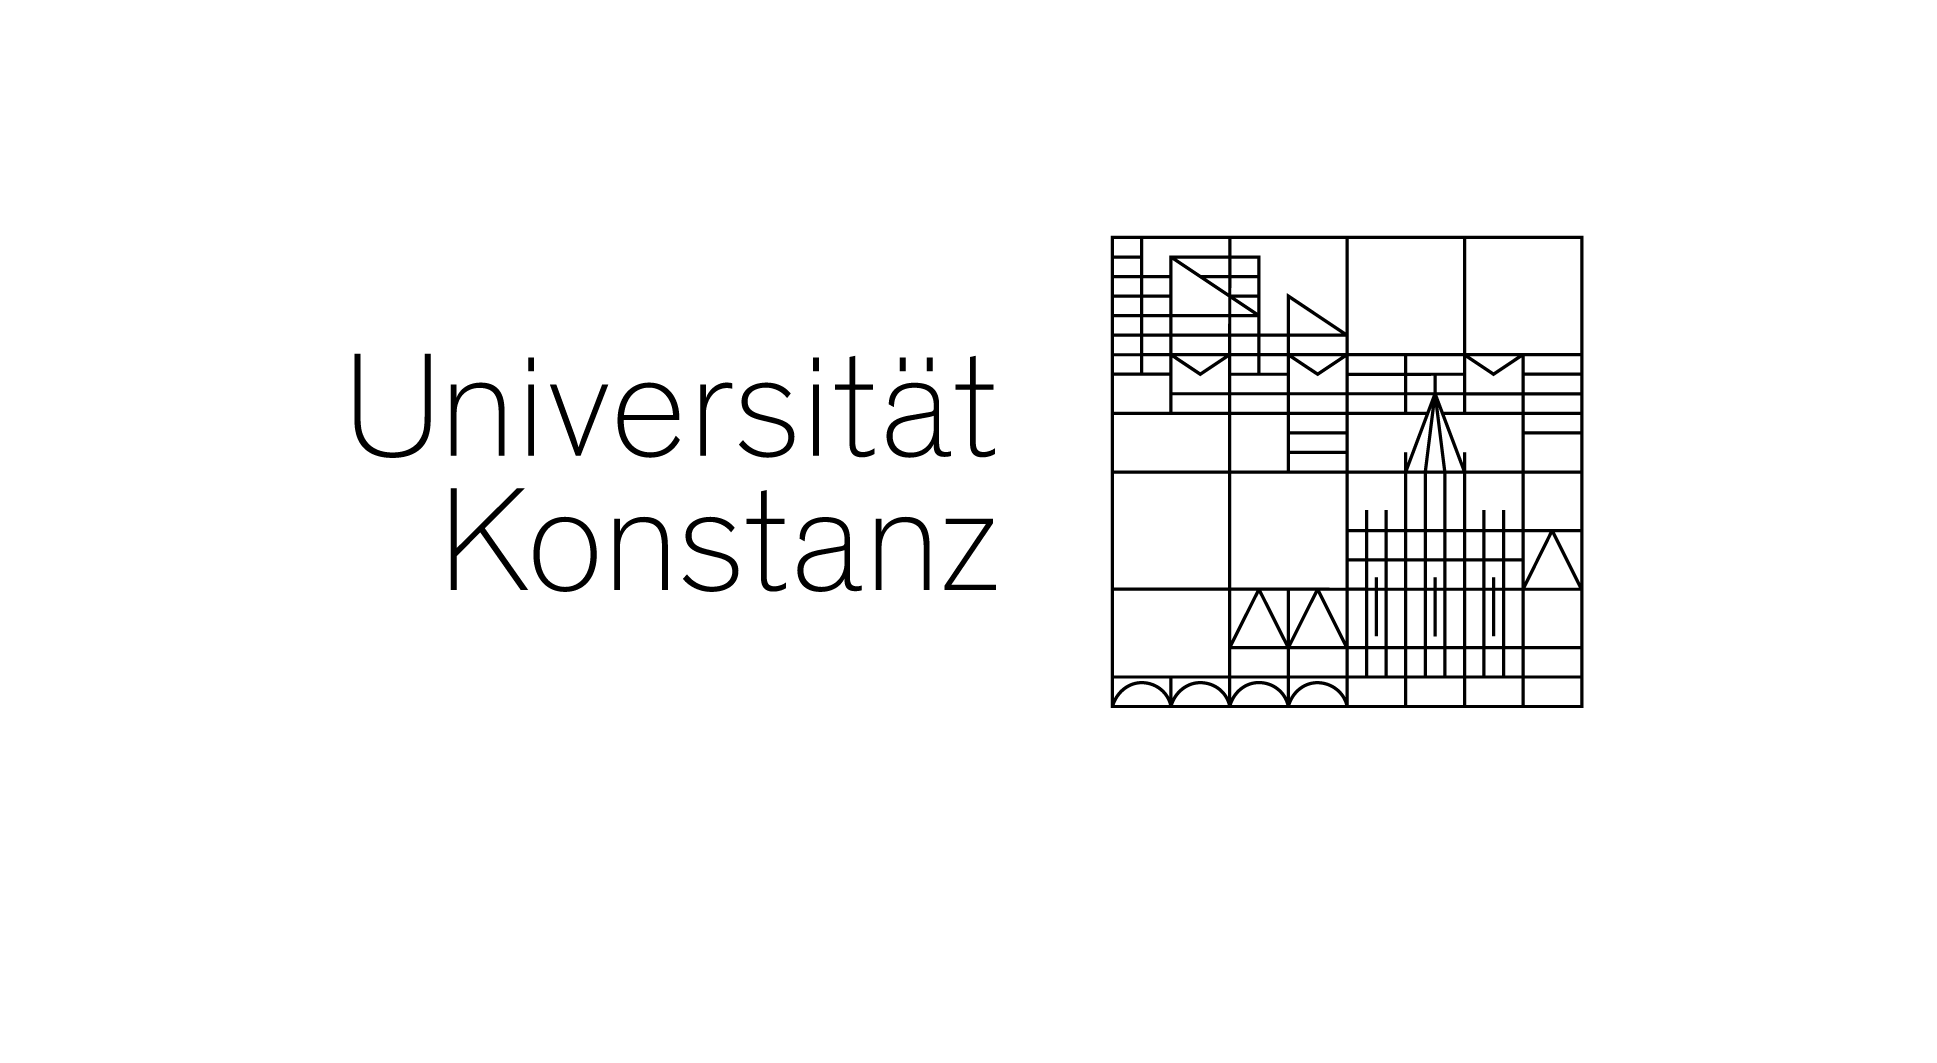
\includegraphics[width=1.2\textwidth]{logounikn} % first figure itself
				
			\end{minipage}\hfill
			\begin{minipage}{0.45\textwidth}
				\centering
				
\includegraphics[width=0.9\textwidth]{bsi_logo} % second figure itself
				
			\end{minipage}
		\end{figure}
		\centering
		\vspace{1cm}
		{\scshape\LARGE Universität Konstanz\\
			\large Fachbereich Mathematik und Statistik\\
			 \& \\ \LARGE Bundesamt für Sicherheit in der Informationstechnik \par}
		\vspace{1cm}
		{\scshape\Large Masterarbeit zum Thema:\par}
		\vspace{0.5cm}
		{\Huge \bfseries Untersuchung \& Entwicklung von Ansätzen zur Detektion von Poisoning-Angriffen\par} %corher wars in \huge, das sah auch nicht so schlecht aus
		\vspace{0.5cm}
		vorgelegt von \par
		\vspace{0.5cm}
		{\Large Lukas Schulth\\
			\texttt{lukas.schulth@uni.kn}\par}
		%\vfill
	
		
		
	
	
		\vspace{1cm}
		unter der Betreuung von\par
		\centering
		\begin{figure}[h]
			
			\makebox[1 \textwidth][c]{   
				\begin{tabular}{ll}
					\pbox{20cm}{Erstkorrektor: \\
						Herr Prof. Dr. Johannes Schropp \\ \texttt{johannes.schropp@uni.kn}} 
					& \pbox{20cm}{Zweitkorrektor:\\
						Herr Prof. Dipl.-Ing. Markus Ullmann\\
						\texttt{markus.ullmann@bsi.bund.de}} \\ 
					&\\
					\pbox{20cm}{Herr Dr. Christian Berghoff \\ \texttt{christian.berghoff@bsi.bund.de}} 
					& \pbox{20cm}{Herr Matthias Neu \\ \texttt{matthias.neu@bsi.bund.de}}
					
				\end{tabular}
			}
		\end{figure}
		%\vfill
		%\vspace{0.25cm}
		% Bottom of the page
		{\large 1. Oktober 2021}
	\end{titlepage}
	
	
		
	\selectlanguage{english}
	\begin{abstract}english\end{abstract}
	\selectlanguage{ngerman}
	\begin{abstract}deutsch\end{abstract}
	TODO:
	\begin{itemize}
		\item Algorithmen aufschreiben
		\item Dreicksungleich und Metrik Beweis Wp(a,b) fertigstellen
		\item Verallgemeinerung auf  verschiedene Räume \cite{vayer2020fused}
	\end{itemize}
	\keywords{one, two, three, four}
	\newpage
	%\thispagestyle{empty} 
	\listoffigures
	
	\listoftables
	
	\lstlistoflistings
	
	\listofalgorithms
	\newpage
	\tableofcontents
	\newpage
	
	
	
	
	\begin{algorithm} 
		\caption{Foo bar} 
		... 
	\end{algorithm} 
	\section{Einführung}
	Allein für Deutschland wird erwartet, dass mit Dienstleistungen und Produkten, die auf dem
	Einsatz von Künstlicher Intelligenz (KI) basieren, im Jahr 2025 Umsätze in Höhe von 488 Milliar­
	den Euro generiert werden – damit würde ein Anteil von 13 Prozent am Bruttoinlandsprodukt
	erreicht. Dabei ist die Erklärbarkeit von Entscheidungen, die durch KI getroffen werden, in
	wichtigen Anwendungsbranchen eine Voraussetzung für die Akzeptanz bei den Nutzenden, für
	Zulassungs- und Zertifizierungsverfahren oder das Einhalten der durch die DSGVO geforderten
	Transparenzpflichten. Die Erklärbarkeit von KI-Produkten gehört damit, zumindest im europäi-
	schen Kontext, zu den wichtigen Markterfolgsfaktoren.[STudieErklärbareKI]
	
	
	
	
	RIght to be forgottten,  General Data Protection Regulation (GDPR) in
	the European Union [5], \url{https://arxiv.org/pdf/2003.04247.pdf}, 5: G. D. P. Regulation, “Regulation (eu) 2016/679 of the
	european parliament and of the council of 27 april 2016
	on the protection of natural persons with regard to the
	processing of personal data and on the free movement
	of such data, and repealing directive 95/46,” Official
	Journal of the European Union (OJ), vol. 59, no. 1-88,
	p. 294, 2016.
	
	Datengewinnung(LRP)
	Datenverarbeitung(kMeans, Gromov Wasserstein)
	Pweave\footnote{\url{https://mpastell.com/pweave/}}
	
	A Complete List of All (arXiv) Adversarial Example Papers \footnote{\url{https://nicholas.carlini.com/writing/2019/all-adversarial-example-papers.html}}
	\\
	In sicherheitskritischen Anwendungsgebieten ist die Erklärung für das Zustandekommen einer Entscheidung genauso wichtig wie die Entscheidung selbst\cite{LRP_DNN}.
	
	Clustering auf Datenpunkten direkt(~50 Prozent = raten), Clustering auf Aktivierungen gut geeigneter Netzwerkschichten. Clustering auf den Heatmaps der verdächtigen Klasse.\\
	\\
	
	Clustering auf unterschiedlichen Repräsentationen der Bilder:
	\begin{itemize}
		\item Clustering direkt auf den Bildern\\
		\item Clustering auf den Activations einer Netzwerkschicht(Im Paper \cite{AC} wird die vorletzte Schicht benutzt)
		\item Clustering auf den Heatmaps
	\end{itemize}
	In \autoref{chapter_nn} geben wir eine kurze Einführung in Neuronale Netzwerke und stellen die untersuchten Modelle vor. \autoref{chapter_poisoningattacks} führt in die unterschiedlichen Möglichkeiten eines Poisoning-Angriffs auf Neuronale Netzwerke ein. \autoref{chapter_xai} gibt eine kurze Übersicht über den Bereich der Erklärbaren Künstlichen Intelligenz, wobei ein Beispiel eines Verfahrens, die sogenannte Layer-wise Relevanz Propagation ausführlich in \autoref{chapter_lrp} vorgestellt wird. Kern der Arbeit bildet \autoref{chapter_algorithm}, wo wir zu Beginn die grundlegenden Bestandteile des Algorithmus zur Detektion von Poisoning-Angriffen auf Neuronale Netzwerke erklären, bevor die experimentellen Ergebnisse in \autoref{chapter_results} ausführen. Ein Vergleich mit anderen Detektionsverfahren wird in \autoref{chapter_comparisons} durchgeführt.
	\section{Neuronale Netzwerke} \label{chapter_nn}
	Wir betrachten ein \gls{nn}, dass die Funktion $f_{\theta}:\mathbb{R}^n \to\mathbb{R}$, mit $\theta = (w_{il}, b_{il})$ beschreibt. 
	i: Schicht
	l: Neuron in der Schicht
	w: Gewichte 
	b: Bias
	g: nichtlineare Akivierungsfunktion
	Architektur,
	Modell
	Pre-Activations(lokal, global): $z_{ij} = x_i*w_{ij}$
	$z_j = \sum_iz_{ij} + b_j$
	
	Vorschrift/aktivierungen: $x_j = g(z_{ij})$
	
	
	Training;testing, Validation, Forward pass, backward pass
	SGD erklärt im Einführungsteil von \cite{BatchNormalization}
	
	fehlende Interpretierbarkeit
	
	ReLUs in den meisten Netzwerken
	
	Definition Klasse
	
	Supervised vs Unsupervised
	
	Dimensionality reduction and Visualisation
	Was ist die letzte/vorletzte Shickht? vgl. Ac
	
	Wir verwenden die Begriffe Bild und Datenpunkt äquivalent.
	\subsubsection{CNNS}
	s. MA Juliane Braunsmann (convolutions /cross correlations)
	Idee, Abstraktion, high level, low level features, bekannte Netzwerke\\
	
	Ausführliche Einführung stanford Kurs\cite{cnn_stanford}. Unterschied zu FC layers: 
	It is worth noting that the only difference between FC and CONV layers is that the neurons in the CONV layer are connected only to a local region in the input, and that many of the neurons in a CONV volume share parameters. However, the neurons in both layers still compute dot products, so their functional form is identical. Therefore, it turns out that it’s possible to convert between FC and CONV layers
	
	Starting with LeNet-5   [10], convolutional neural networks (CNN) have typically had a standardstructure – stacked convolutional layers (optionally followed by contrast normalization and max-pooling)  are  followed  by  one  or  more  fully-connected  layers.   Variants  of  this  basic  design  areprevalent in the image classification literature and have yielded the best results to-date on MNIST,CIFAR and most notably on the ImageNet classification challenge [9, 21].  For larger datasets suchas Imagenet, the recent trend has been to increase the number of layers  [12] and layer size [21, 14],while using dropout [7] to address the problem of overfitting.\cite{goingdeeperwithconvolutions}
	
	Softmax am Ende für Transformation in Probabilities.
	
	Netzwerk im Netzwerk \cite{cnn_architectures_stanford, goingdeeperwithconvolutions}
	
	\subsubsection{Besondere Schichten}
	Promotion Sebastian Lapuschkin
	
	\begin{itemize}
		\item \textit{BatchConv} besteht aus 
		\begin{lstlisting}[language=Python, caption=python-interner Aufbau einer BatchConv Schicht
		]
		nn.Conv2d(in_channels=in_channels, out_channels=out_channels, **kwargs)
		nn.BatchNorm2d(num_features=out_channels)
		nn.ReLU()
		\end{lstlisting}
		in genau dieser Reihenfolge
		Bem.: Nur für BatchNorm2d müsste man LRP implementieren, für Conv2d funktioniert das bereits.
	\end{itemize}
	
	Batch Normalization\footnote{\url{https://arxiv.org/pdf/1502.03167.pdf}}
	
	
	\subsubsection{Inception v3}
	Filter,
	In Klassischen feed forward Netzen wird Output der vorheigen layer ist input der nächsten layer
	
	Jetzt: Inception Block: Previous layer input, 4 operations in parallel, concatenation,1x1 conv -> lower dimension -> less computational cost
	
	Intermediate classifiers: kommt aus multitask learning. Eigentlich eine Möglickeit gegen vasnishing gradients
	
	\subsubsection{VGG16}
	VGG16 is a convolutional neural network model proposed by K. Simonyan and A. Zisserman from the University of Oxford in the paper Very Deep Convolutional Networks for Large-Scale Image Recognition. The model achieves 92.7\% top-5 test accuracy in ImageNet, which is a dataset of over 14 million images belonging to 1000 classes. It was one of the famous model submitted to ILSVRC-2014. It makes the improvement over AlexNet by replacing large kernel-sized filters (11 and 5 in the first and second convolutional layer, respectively) with multiple 3×3 kernel-sized filters one after another. VGG16 was trained for weeks and was using NVIDIA Titan Black GP’s.%\cite{vgg16_neurohive} \cite{vgg16_architecture}
	
	\subsection{Datensatz}
	GTSRB\footnote{\url{https://benchmark.ini.rub.de/gtsrb_dataset.html}}
	
	Für die Poisoning-Angriffe auf verschiedene neuronale Netzwerke benutzen wir
	den Datensatz German Traffic Sign Recognition Benchmark 1 . Dieser besteht
	aus 52.001 Bildern von Verkehrsschildern aus 43 verschiedenen Kategorien der
	Pixelgröße 32x32. Etwa 75 Prozent der Bilder wird für das Training, die ande-
	ren 25 Prozent für das Testen benutzt. Der Datensatz wurde ursprünglich in
	einem Wettbewerb auf der International Joint Conference on Neural Networks
	(IJCNN) im Jahr 2011 benutzt. Die Bilder sind aus aus einer Videosequenz
	herausgeschnitten. Deshalb befinden sich in einer Klasse jeweils immer meh-
	rere Bilder desselben Verkehrsschildes zu unterschiedlichen Zeitpunkten. Auf-
	nahmen desselben Verkehrsschildes kommen nicht übergreifend in Training-,
	Validierung- oder Testdatensatz vor.
	Verkehrsschild
	\begin{table}[h]
		\begin{tabular}[h]{c|c}
			Verkehrsschilder & Anzahl an Bildern \\ \hline
			’Zulässige Höchstgeschwindigkeit: 20km/h’& 180 \\
			’Zulässige Höchstgeschwindigkeit: 30km/h’ & 1980 \\
			’Zulässige Höchstgeschwindigkeit: 50km/h’	& 2010 \\
			’Zulässige Höchstgeschwindigkeit: 60km/h’	& 1260 \\
			’Zulässige Höchstgeschwindigkeit: 70km/h’	& 1770 \\
			’Zulässige Höchstgeschwindigkeit: 80km/h’	&1650 \\
			’Halt! Vorfahrt gewähren’					&	690
		\end{tabular}
		\label{tab:Auswahl_Datensatz}
		\caption{Für einen Poisoning-Angriff interessante Klassen und die zugehörige Anzahl an Bildern.}
	\end{table}
	
	
	
	
	
	
	
	
	In \autoref{tab:Auswahl_Datensatz} sind einige Klassen der Verkehrsschilder und deren An-
	zahl im Datensatz aufgelistet, die für einen Poisoning-Angriff interessant sein
	könnten. Die Anzahl der Schilder ’Halt! Vorfahrt gewähren’-Schilder im Trainingssatz beträgt etwa 690 Aufnahmen. Diese wurden von insgesamt nur 24 verschiedenen ’Halt! Vorfahrt gewähren’-Schildern aufgenommen. Da beim Erstel-
	len der korrumpierten Daten auch immer das Bild aus der angegriffenen Klasse
	in die Zielklasse verschoben wird, wird die Anzahl der in der Ursprungsklasse verbleibenden Daten abhängig vom Anteil an korrumpierten Daten kleiner.
	Wir werden uns deshalb im Folgenden mit Angriffen auf die Klasse ’Zulässige
	Höchstgeschwindigkeit: 50 km/h’ beschäftigen, da sie die höchste Anzahl an
	Daten aufweist.
	
	
	\section{Poisoning-Angriffe} \label{chapter_poisoningattacks}
	Gute BEschreibung in 3.Method \url{https://arxiv.org/pdf/1910.00033.pdf}
	Mithilfe eines manipulierten Datensatzes wird das Netzwerk manipuliert, sodass die Entscheidung des Netzwerkes abhängig von einem Auslöser ist.
	
	\noindent \textbf{Wer wird wie angegriffen?}: Der Angreifer erstellt einen Datensatz, sodass in den Netzwerken, die auf diesem Datensatz trainiert werden eine Hintertür implementiert wird. Damit ergibt sich die Annahme, dass der Angreifer volle Kontrolle über den Datensatz hat und somit Datenpunkte entfernen oder hinzufügen kann.
	
	Was passiert, wenn der Angreifer keinen Zugriff auf die Modell-Architektur hat? Transfer-Learning? 
	
	\noindent \textbf{Anbringen des Auslösers}
	\subsection{Standard Poisoning-Angriffe}
	Wir wollen Schilder der Klasse 50kmh absichtlich falsch als 80kmh. Wir wählen diese beiden Klassen aufgrunde der Größe beider Klassen(s. Aufstellung in Praktikumsbericht). Stoppschildklasse ist wohl vergleichsweise ze8imlich klein.\\
	
	Dazu fügen wir auf den 50er Schildern einen Sticker ein und ändern das Label auf 80.
	Label-Consistent
	Backdoor Attacks
	Für die Bewertung, wie erfolgreich ein Angriff war, fügen wir in jedem Bild der 50er Klasse im Testdatensatz einen Sticker ein und messen, wie groß der Anteil der 50er Schilder ist, die als 80er Schild klassifiziert werden.\\
	
	\noindent \textbf{CH- und Backdoor-Artefakte}:\\
	In \cite{imagenet_unhansed_v2} wird wie folgt zwischen Clever Hans- und Backdoor-Artefakten unterschieden. In beiden Fällen wird rechts oben im Bild ein grauer 3x3 Sticker eingefügt.
	Bei CH geschieht dies bei $25 \%$ der "airplane"-Klasse. Bei Backdoor-Artefakten werden $10 \%$ aller Bilder korrumpiert. Im zweiten Fall wird das entspechende Label abgeändert. Dies entspricht dann einem Standard- bzw. Clean-Label-Poisoning-Angriff. (Wie git funktioniert der CLPA/CH hier ohne die Bilder vorher schlechter zu machen? TODO: Vergleich mit \cite{labelconsistent}). In \cite{imagenet_unhansed_v2}, Kapitel 2.1 wird auch auf die Methode der Spektralen Signatur \cite{spectral_signatures} eingegangen, die zur Detektion genutzt wird. Diese eignet sich wohl sehr gut für die Backdoor-Attacks, aber nur schlecht für die CH-Artefakte.
	
	
	\subsection{Label-konsistente Poisoning-Angriffe}
	Bei den vorheringen Standard-Angriffen war es der Fall, dass das Label und das entsprechende Bild nicht mehr zusammenpassen. Ein händisches Durchsuchen des Datensatz (wenn auch sehr aufwendig) könnte damit ebenfalls zur Detektion eines Angriffs führen.\\
	Eine deutlich schwieriger zu detektierende Art von Poisoning-Angriffen sind sogenannte Label-konsistente Angriffe, bei denen genau diese Schwachstelle eliminiert ist, d.h. Label und Bild passen wieder zueinander, während der Angriff noch immer erfolgreich funktioniert. Es ist das Ziel, ein Bild zunächst so zu modifizieren, dass es für das menschliche Auge noch immer zur entsprechenden Klasse gehört,für das Neuronale Netzwerk aber so schwierig zu klassifizieren ist, dass sich das Netzwerk eher auf den Auslöser anstatt auf das ursprüngliche Bild verlässt. Im Anschluss wird wieder ein Auslöser eingefügt.\\
		
	In \cite{labelconsistent} werden zwei Verfahren vorgestellt, die die Klassifikation einzelner Bilder erschweren. Das erste Verfahren besteht aus einer Einbettung in einen niedrig-dimensionalen Raum, das auch bei Autoencodern, etc. verwendet wird TODO.
	
	Beim zweiten Verfahren wird ein sogenannte Projizierter Gradienten-Abstieg-Angriff durchgeführt.\\
	Dabei wird ein Adversarialer Angriff in leicht abgewandelter Form genutzt, um das Netzwerk zu stören. Bei Adversarialen Angriffen wird ein Netzwerk im Unterschied zum Poisoning-Angriff, bei dem der Angriff während des Trainings stattfindet, nach dem Training angegriffen. Dazu wird eine natürliche Netzwerkeingabe leicht gestört, sodass diese vom Netzwerk falsch klassifiziert wird. Diese Störungen lassen sich auch von einer Architektur oder sogar einem Modell auf andere übertragen \cite{szegedy2013intriguing, papernot2016transferability}.
	%TODO: Unterschied zw. Klassifizierung und Klassifikation
	Für diese Art von Angriff werden die adversarialen Angriffe und ihre leichte Übertragbarkeit auf andere Architekturen und Modelle so benutzt, dass es bereits während des Trainings zu falschen Klassifikationen kommt.\\
	Für unser erstes trainiertes Netzwerk $f_\theta$ mit Verlustfunktion $\mathcal{L}$ und einem Eingabe-Paar $(x,y)$, konstruieren wir die modifzierte Version von $x$ als
	\begin{equation}
		x_{adv} = \argmax_{||x'-x||_p \leq \varepsilon}{\mathcal{L}(x',y,\theta},
	\end{equation}
	
	für $p >1 $ und $\varepsilon > 0$. Dieses Optimierungsproblem wir mit einem Projizierten Gradienten-Verfahren \cite{madry2017towards}. Details dazu finden sich in \autoref{param_attacks}. Im Unterschied zu \cite{labelconsistent} ändern wir nur Bilder im Datensatz ab und fügen nicht zusätzlich zum Original $x$ auch $x_{adv}$ hinzu. Damit ändert sich die Anzahl an Datenpunkten durch den Angriff nicht.
	
	Für das anschließende Einfügen des Auslöser ergeben sich die folgenden Optionen:
	\begin{itemize}
		\item Der im Standard-Angriff verwendete Sticker
		\item Ein Amplitudensticker: Dabei wird im rechten unteren Eck des Bildes ein 
		\item Amplitudensticker 4 fach
		\item In die Mitte verschobene Amplitudensticker
	\end{itemize}
	RGB auf jedem Kanal in der range von [0,255]
	0 entspricht weiß, 255=schwarz
	Da die zweite Möglichkeit als deutlich erfolgreicher angegeben wird, beschränken wir uns auf diese Angriffe basierend auf einem Projizierten Gradienten-Abstieg.
	amp=16,32,64,255
	Wir gehen zunächst davon aus, dass der Angreifer volle Kontrolle über den Datensatz und das Netzwerk besitzt.TODO: Angriff mit einem andere Netzwerk erstellen, als das angegriffene
	
	\subsection{Bewertung von Poisoning-Angriffen}
	
	Wann ist ein Angriff erfolgreich?\\
	Im Trainingsdatensatz werden im Fall des Standard-Angriffs alle Bilder mit dem Sticker versehen. Die Angriffserfolgsrate beschreibt nun den Anteil an Bildern der attackierten Klasse, die erfolgreich falsch klassifiziert wurden.\\
	
	Für die Label-konsistenten Angriffe werden im Test-Datensatz alle Bilder mit dem entsprechenden Auslöser versehen und es kann eine Erfolgsrate pro Klasse berechnet werden. Es ist zu beachten, dass für Angriffe, die mit einer reduzierten Amplitudenstärke durchgeführt werden, die Bilder im Test-Datensatz dennoch mit Auslösern mit voller Amplitudenstärke versehen werden. 
	
	\subsection{Verteidigungen}
	In diesem Kapitel beschäftigen wir uns mit gängigen Methoden zur Detektion von Poisoning-Attacks und geben am Ende einen kurzen Ausblick auf die Idee für einen neuen Ansatz.
	Wir wollen beide Arten von Poisoning-Angriffen erfolgreich detektieren. 
	
	\subsubsection{Referenzwert: kMeans(k=2)}
	Der einfachste Ansatz, um korrumpierte Datenpunkte zu erkennen, ist ein kMeans-Clustering, das direkt(bzw. nach einer Dimensionsreduktion) auf den Eingabedaten einer Klasse durchgeführt wird. Hierbei war auffällig, dass der Großteil der Daten als korrumpiert klassifiziert wurde. Für die Dimensionsreduktionen FastICA und PCA ergab sich eine Genauigkeit von etwa $66 \%$. Die FPR lag bei über 70 \%, die TPR bei ca. $50 \%$.
	Dieser Referenzwert w@article{szegedy2013intriguing,
		title={Intriguing properties of neural networks},
		author={Szegedy, Christian and Zaremba, Wojciech and Sutskever, Ilya and Bruna, Joan and Erhan, Dumitru and Goodfellow, Ian and Fergus, Rob},
		journal={arXiv preprint arXiv:1312.6199},
		year={2013}
	}
	urde für einen Sticker mit Seitenlänge 3 und $15 \%$ korrumpierten Daten durchgeführt.
	\subsubsection{Activation Clustering}
	
	
		Nehme Datensatz her
		Beim Standardangriff wollen wir Klasse 5 als Klasse 8 klassifzieren und fügen dazu Sticker der  
		
		
		Diese Idee der Verteidigung basiert auf der Annahme, dass bestimmte Schichten innerhalb des Netzwerkes die Entscheidung, dass ein Bild mit einem Auslöser falsch klassifiziert wird, sehr gut codieren. Für die Detektion der Hintertüren im Datensatz sollen nun genau diese Aktivierungen für ein Clustering herangezogen werden.
		Das Activation Clustering wird erstmalig in \cite{AC} vorgestellt und nutzt aufgrund experimenteller Untersuchungen stets die Aktivierungen der vorletzten Netzwerkschicht.
		Eine Kombination von Aktivierungen mehrere Schichten wäre ebenfalls denkbar.
				
		Ein Angriff ist erfolgreich, wenn eine große Anzahl an Datenpunkten der Ur-
		sprungsklasse, versehen mit einem Auslöser, der Zielklasse zugeordnet werden.
		Im Falle eines erfolgreichen Angriffs werden korrumpierte und nicht korrumpier-
		te Datenpunkte im Trainingsdatensatz derselben Klasse zugeordnet. Der Grund
		weshalb diese derselben Klasse zugeordnet werden, unterscheidet sich jedoch.
		Beim Activation Clustering wird nun angenommen, dass pro Klasse entweder
		korrumpierte und nicht korrumpierte Datenpunkte oder nur nicht korrumpierte
		Datenpunkte existieren. Deshalb werden die Aktivierungen der letzten verdeck-
		ten Schicht des Netzwerkes aus dem Netz extrahiert, nach ihren zugehörigen
		Klassen der Labels segmentiert, auf 10 Dimensionen reduziert und anschließend
		mit Hilfe des kMeans-Algorithmus geclustert. Das kleinere Cluster wird immer
		als der Anteil an verdächtigen Datenpunkten betrachtet. Die Idee ist es, dass
		die korrumpierten Datenpunkte, sofern welche existieren, alle in die eine und
		die nicht korrumpierten Datenpunkte in das andere Cluster aufgeteilt werden.
		Sind keine korrumpierten Datenpunkte vorhanden, so sollen beide Cluster un-
		gefähr dieselbe Anzahl an Datenpunkten erhalten.\\
		
		Wir werten die Qualität des Clusterings anschließend aus. Als Detektionsrate
		beschreiben wir die Genauigkeit des Clusterings auf den Trainingsdaten.
		
		Im folgenden Abschnitt werden Methoden vorgestellt, mit denen das resultierende Clustering auf die präsenz eines Angriffs untersucht werden kann. Dies ist notwendig, da in der Praxis ein Angriff zunächst erkannt und anschließend die korrumpierten Datenpunkte entfernt werden müssen. 
		
		\begin{remark}
			Das SPA benutz die Idee das innerhalb einer Klasse bezüglich unterschiedlicher Aktivierungen klassifiziert werden kann. Beim CLPA funktioniert das nicht mehr, denn: Hier passen jetzt auch die Aktivierungen der korrumpierten Bilder zur entsprechenden/untersuchten Klasse. Es ist also zu erwarten, dass das AC für CLPA nicht funktioniert.
		\end{remark}
	
		\subsection{Implementierung}
		Wir nutzen die python Implementierun in sklearn mit den Standard-Werten $n\_init=10$ und $max\_iter=300$
		
		
		\subsubsection{Methoden zur Untersuchung, ob ein Angriff vorliegt}
		\#TODO: Vergleich mit Fisher-Discriminant-Anaylsis/Ansatz in \cite{imagenet_unhansed_v1}
		Zur
		Bestimmung, ob eine Klasse korrumpierte Daten enthält, kann das Ergebnis
		des Clusterings mit den folgenden Methoden untersucht werden:\\
		
		\noindent \textbf@article{szegedy2013intriguing,
			title={Intriguing properties of neural networks},
			author={Szegedy, Christian and Zaremba, Wojciech and Sutskever, Ilya and Bruna, Joan and Erhan, Dumitru and Goodfellow, Ian and Fergus, Rob},
			journal={arXiv preprint arXiv:1312.6199},
			year={2013}
		}
		{Vergleich der relativen Größe:} Eine Möglichkeit, korrumpierte Datenpunkte
		zu erkennen, ist der Vergleich der relativen Größen der beiden Cluster. Laut [2]
		ist die relative Größe bei nicht korrumpierten Klassen ca. 50 Prozent, bei kor-
		rumpierten Daten und einem erfolgreichen Clustering würde die relative Größe
		dann dem prozentualen Anteil an korrumpierten Datenpunkten entsprechen.\\
		
		\noindent \textbf{Silhouette-Koeffizient:} Eine weitere Möglichkeit besteht darin, die Qualität
		des Clusterings mit Hilfe des Silhouette-Koeffizienten zu beschreiben. Dieser gibt
		an, wie gut ein Clustering zu den gegebenen Datenpunkten mit den entsprechen-
		den Labeln passt und ist wie folgt definiert: Sei das Ergebnis eines Clustering-
		Algorithmus mit verschiedenen Clustern gegeben. Zu einer Beobachtung $x$ im Cluster $A$ wir die Silhouette $s(x) = \frac{d(B,x)-d(A,x)}{max\lbrace d(A,x), d(B,x) \rbrace}$ definiert, wobei $d(A,x)  = \frac{1}{n_A -1}\sum_{a \in A, a \neq x}{d(a,x)}$ dem mittleren Abstand einer Beobachtung innerhalb einer Klasse zu allen anderen Beobachtungen dieser Klasse entspricht.
		Dabei steht $n_A$ für die Anzahl der Beobachtungen in Cluster A. $d(B,x) = \min_{C \neq A}d(C,x)$ beschreibt die Distanz von $x$ zum nächstgelegenen Cluster B. Der Silhouetten-Koeffizient $SC$ ist nun definiert als
		\begin{equation}
			SC = \max_k \tilde{s}(k),
		\end{equation}
		wobei $\tilde{s}(k)$ der Mittelwert der Silhoutten aller Datenpunkte im gesamten Datensatz ist. Damit ist der Silhouttenkoeffizient ein Maß dafür, wie gut ein Clustering für eine vorher fixierte Clusteranzahl $k$ zum Datensatz passt.\\
		
		\noindent \textbf{Exklusives Retraining:} Beim exklusiven Retraining wird das neuronale Netz
		von Grund auf neu trainiert. Das oder die verdächtigen Cluster werden beim
		erneuten Training nicht benutzt. Mit Hilfe des neu trainierten Netzes wer-
		den dann anschließend die vorenthaltenen, verdächtigen Cluster klassifiziert.
		Falls das Cluster Aktivierungen von Datenpunkten enthält, die zum Label des
		Datenpunktes gehören, erwarten wir, dass die Vorhersage des Netzwerks mit
		dem Label übereinstimmen. Gehören die Aktivierungen eines Datenpunktes im
		verdächtigen Cluster jedoch zu einer anderen Klasse als die durch das Label
		angedeutete Klasse, so sollte das Netzwerk den Datenpunkt einer anderen Klas-
		se zuordnen. Um nun zu entscheiden, ob ein verdächtiges Cluster korrumpiert
		oder nicht korrumpiert ist, wird wie folgt vorgegangen: Sei $l$ die Anzahl an Vor-
		hersagen, die zum Label des Datenpunktes passen. Sei $p$ die größte Anzahl an
		Vorhersagen, die für eine weitere Klasse $C$ sprechen, wobei $C$ nicht die Klas-
		se mit den Labeln des zu untersuchenden Clusters ist. Der Quotient $\frac{l}{p}$ gibt
		dann an, ob das Cluster korrumpiert ist oder nicht: Es wird ein Schwellenwert
		$T > 0$ gesetzt. Gilt $\frac{l}{p} < T$ , wurden mehr Datenpunkte einer anderen Klasse zu-
		geordnet und das Cluster wird als korrumpiert deklariert. Umgekehrt wird das
		verdächtige Cluster im Fall von $\frac{l}{p} > T$ als nicht korrumpiert/sauber eingestuft.
		@article{szegedy2013intriguing,
			title={Intriguing properties of neural networks},
			author={Szegedy, Christian and Zaremba, Wojciech and Sutskever, Ilya and Bruna, Joan and Erhan, Dumitru and Goodfellow, Ian and Fergus, Rob},
			journal={arXiv preprint arXiv:1312.6199},
			year={2013}
		}
		
		\subsubsection{Entfernen von korrumpierten Datenpunkten}
	
	\noindent \textbf{AC für Label-konistente Poisoning-Angriffe:} Warum funktioniert Activation-Clustering hier nur schlecht oder gar nicht?: Wenn wir einen korrumpierten Trainingsdatensatz gegeben haben, gilt im Fall des Standard-Angriffs folgender Sachverhalt: Die angegriffene Klasse, die Klasse in der samples eingefügt wurden, besitzt die eine Gruppe an Bildern, die zu einer Aktivierung von einer anderen Klasse führen sollten, und die Gruppe an Bildern, die zu dieser Klasse gehören und zur Aktivierung genau dieser Klasse führen sollte.\\
	Im Fall des Label-konsistenten Poisoning-Angriffs, werden nun keine Label mehr getauscht, d.h. Bilder von der einen in die andere Klasse verschoben. Damit können die beiden Gruppen (korrumpiert, sauber) innerhalb einer Klasse nicht mehr anhand ihrer Aktivierungen unterschieden werden.\\
	Trotzdem ergibt sich ein Ansatz daraus, dass es innerhalb dieser Klasse verschiedene \glqq Strategien\grqq{}  gibt, die zur selben Klassifikation führen. Mithilfe des kmeans-Clustering basierend auf den Heatmaps sollen genau diese Strategien ausfindig gemacht werden, um die Bilder in korrumpiert und sauber zu unterteilen.
	
	\subsubsection{Heatmap Clustering}
	Im Unterschied zum Activation Clustering, bei dem die Aktivierungen der vorletzten Netzwerk-Schicht verwendet werden, ist nun hier die Idee, zu jedem Eingabebild eine Relevanzkarte zu erstellen, die für jeden Pixelpunkt angibt, wie wichtig dieser für die Klassifikation dieses Bildes ist. \\
	
	Für das Erstellen/Berechnen solcher Relevanzkarten/Heatmaps existieren mehrere Methoden, die zusammengefasst dem Bereich der Erklärbaren KI zugeordnet werden.
	Im folgenden Kaptiel wollen wir einen kurzen Überblick über verschiedene Methoden geben.
	
	
	\section{Erklärbare KI} \label{chapter_xai}
	
	Erklärbarkeit vs. Interpretierbarkeit, youtube talk?!
	
	
	Den Kern von KI-basierten Anwendungen – womit hier im Wesentlichen Anwendungen des
	maschinellen Lernens gemeint sind – bilden immer die jeweils zugrundeliegenden KI-Modelle.
	Diese lassen sich in zwei Klassen einteilen: White- und Black-Box-Modelle. White-Box-Modelle,
	wie bspw. auf nachvollziehbaren Eingangsgrößen basierende Entscheidungsbäume, erlauben
	das grundsätzliche Nachvollziehen ihrer algorithmischen Zusammenhänge; sie sind somit
	selbsterklärend in Bezug auf ihre Wirkmechanismen und die von ihnen getroffenen Entscheidun-
	gen. Bei Black-Box-Modellen wie neuronalen Netzen ist es aufgrund ihrer Verflechtung und Viel-
	schichtigkeit in der Regel nicht mehr möglich, die innere Funktionsweise des Modells nachzu-
	vollziehen. Zumindest für die Erklärung von Einzelentscheidungen (lokale Erklärbarkeit) können
	dann jedoch zusätzliche Erklärungswerkzeuge eingesetzt werden, um nachträglich die Nachvoll-
	ziehbarkeit zu erhöhen. KI-Entwickler können für Entscheidungserklärungen je nach den
	konkreten Anforderungen auf etablierte Erklärungswerkzeuge zurückgreifen, bspw. LIME, SHAP,
	Integrated Gradients, LRP, DeepLift oder GradCAM, die allerdings Expertenwissen voraussetzen.
	Für die Nutzenden existieren bislang nur wenig gute Werkzeuge, die intuitiv verständliche Ent-
	scheidungserklärungen liefern (Saliency Maps, Counterfactual Explanations, Prototypen oder
	Surrogat-Modelle).
	
	\noindent \textbf{Transparenz: }
	Transparenz wird im Folgenden als eine Modelleigen-
	schaft behandelt. Ist die Transparenz eines Modells
	gegeben, so ist es unter der Annahme nachvollziehbarer
	Eingangsgrößen selbsterklärend 4 . Die Eigenschaft der
	Transparenz lässt sich weiter unterteilen in die drei un-
	terschiedlichen Ausprägungen der „Simulierbarkeit“, der
	„Unterteilbarkeit“ und der „Algorithmischen Transparenz“
	(Lipton 2016). Dabei wird in der Literatur häufig von einer
	hierarchischen Abhängigkeit ausgegangen (Arrieta et al.
	2019), sodass die Simulierbarkeit eines Systems dessen
	Unterteilbarkeit und dessen algorithmische Transparenz
	impliziert. Entsprechend begründet die Unterteilbarkeit
	eines Systems auch dessen algorithmische Transpa-
	renz. Folglich gilt ein Modell – unter der Annahme erklär-
	barer Eingangsdaten – bereits als transparent, wenn es
	lediglich die Eigenschaft der algorithmischen Transpa-
	renz erfüllt. Die höchste Transparenzstufe erreicht ein
	Modell, wenn es die Eigenschaft der Simulierbarkeit und
	somit auch die beiden anderen
	Eigenschaften erfüllt.
	
	Ein System ist simulierbar, wenn
	auch eine Person die Entschei-
	dungen des zugrundeliegenden
	Algorithmus in angemessener
	Zeit nachvollziehen kann oder
	könnte, indem sie die einzelnen
	Schritte, die zur Herbeiführung
	einer Entscheidung nötig sind,
	manuell durchführt.	
	
	Beispiel: Beim manuellen
	Durchlaufen unterschiedlicher
	Pfade eines nicht allzu großen
	Entscheidungsbaumes, der auf
	nachvollziehbaren Eingangsgrö-
	ßen beruht, kann eine Person in
	jedem Knoten selbst überprüfen,
	ob eine individuelle Eigenschaft
	von Eingangsdaten bzw. ein Attribut erfüllt ist oder nicht.
	Gibt es keine Attribute mehr zu prüfen, hat die Person
	ein „Blatt“ des Entscheidungsbaums erreicht, welches
	das Ergebnis repräsentiert. 
	
	\noindent \textbf{Erklärbarkeit: }Da Transparenz für diverse Modelle wie z. B. neuronale
	Netze nicht erreichbar ist, diese folglich nicht selbst-
	erklärend sind, kommt bei diesen das Konzept der „Er-
	klärbarkeit“ zur Anwendung. Dabei ist zwar in der Regel
	festgelegt, ob die Erklärbarkeit eine Entscheidung oder
	ein Modell betrifft. Wie eine konkrete Erklärung dabei
	ausgestaltet ist oder wieviel Erkenntnis sie der Zielper-
	son gewährt, bleibt dabei jedoch zunächst unbestimmt.
	Beim Beispiel der Bildverarbeitung mit neuronalen Net-
	zen spricht man etwa bereits von einer Erklärung einer
	Entscheidung, wenn bestimmte Bereiche im Eingabe-
	bild, die zur Klassifikation eines konkreten Objektes ge-
	führt haben, für die anwendende Person farblich hervor-
	gehoben werden. In diesem Fall wird nicht jeder einzelne
	Schritt des Algorithmus erklärt, sondern nur die für die
	Entscheidungsfindung bedeutsamsten Daten hervor-
	gehoben. Alternativ kann eine Erklärung auch durch eine
	textliche Beschreibung repräsentiert werden, z. B. „Auf
	diesem Bild ist ein Hund abgebildet, da vier Beine, eine
	Schnauze, Fell und ein Schwanz erkannt wurden.“
	
	Grundsätzlich wird zwischen zwei Arten von Erklärungen unterschieden:
	
	\begin{itemize}
		\item Erklärungen von Einzelentscheidungen bzw. Ent-
		scheidungserklärungen, die dabei helfen, individuelle,
		datenbezogene Entscheidungen konkret nachzuvoll-
		ziehen (sogenannte lokale Erklärbarkeit oder Daten-
		erklärbarkeit).
		\item Erklärungen von Modellen bzw. Modellerklärungen,
		die dabei helfen, Wirkzusammenhänge von KI-Mo-
		dellen zu begreifen (sogenannte globale Erklärbarkeit
		oder Modellerklärbarkeit), z. B. lineare oder allgemein
		funktionale Zusammenhänge zwischen Eingangs-
		und Ausgangsgrößen.
	\end{itemize}

In den folgenden beiden Abschnitten stellen wir einige der bekanntesten Methoden aus beiden Bereichen vor.


	\noindent \textbf{text}
	\subsection{Lokale Methoden}
	Mithilfe sogenannter Attribution Methods wird der
	negative oder positive Einfluss von Teilen oder Berei-
	chen der Eingabe eines KI-Modells auf dessen Ausgabe
	betrachtet (Sundararajan et al. 2017). Dieser Gruppe
	können die folgenden konkreten Methoden zugeordnet
	werden: Sensitivitätsanalyse, LRP, DeepLIFT, Integrated
	Gradients, Grad-CAM, Guided Backpropagation und
	Deconvolution. Anhand eines gemeinsamen Beispiels
	wird die Funktionsweise erläutert. Die Unterschiede
	sind in den nachfolgenden technischen Einzelheiten
	beschrieben.
	
	\noindent \textbf{CAM / Grad-CAM / Grad-CAM++ (Gra-
		dient-weighted Class Activation Mapping)}
	CAM ist eine Methode zur Visualisierung von ausschlag-
	gebenden Regionen für ein konkretes Klassifizierungser-
	gebnis eines neuronalen Netzes, insbesondere Convo-
	lutional Neural Network (CNN). Das Ergebnis ist eine
	Saliency Map, die über das ursprüngliche Bild gelegt
	werden kann und die betreffenden Regionen hervorhebt.
	Für die Erstellung der Saliency Map werden jeweils nur
	die letzten Schichten (Layer) des Netzes betrachtet.
	CAM ist nicht für jede Netzwerkarchitektur direkt an-
	wendbar; unter Umständen muss diese durch Hinzu-
	fügen weiterer Schichten zuvor angepasst und dann das
	Netz neu trainiert werden.
	Grad-CAM ist eine Generalisierung der CAM-Methode,
	erfordert kein erneutes Training des Modells und ist auf
	mehr Netzwerkarchitekturen anwendbar. Ein Nachteil
	von Grad-CAM ist jedoch, dass nicht mehrere Vor-
	kommen eines Objekts in einem Bild erkannt werden
	können. Grad-CAM++ löst dieses Problem, sodass das
	Erkennen von mehreren Objektinstanzen in einem Bild
	möglich wird.
	
	
	\noindent \textbf{LRP (Layer-Wise Relevance Propagation)}
	Durch LRP wird der Einfluss einzelner Eingaben auf das
		Ergebnis einer Klassifikation betrachtet. Der Fokus liegt
		hierbei auf nicht linearen Klassifizierern wie neuronalen
		Netzen. Betrachtet man die Bildklassifikation, so ist das
		Ziel, für einzelne Bilder herauszufinden, welche Pixel in
		welchem Umfang das Klassifizierungsergebnis positiv
		oder negativ beeinflussen. Jedem Inputwert (hier: Pixel)
		wird ein Relevanzwert zugeordnet. Der Wert der „Rele-
		vanz“ gibt an, wie groß der Einfluss eines Eingabewerts
		oder einer Unit des Netzes auf das Klassifikationsergeb-
		nis ist. Der Relevanzwert der Ausgabe setzt sich aus der
		Summe der Relevanzwerte der Eingabewerte zusam-
		men. Der Ausgabewert des Netzes wird also „zerlegt“ in
		die jeweiligen Beiträge (bzw. den Einfluss) der Eingabe-
		werte (= Dekomposition). Die Berechnung der Relevanz
		der Eingabewerte wird iterativ von hinten (letzter Layer)
		nach vorn (Input-Layer) ausgeführt.
	
	\noindent\textbf{IG (Integrated Gradients)}
	Diese Methode ist ebenfalls zur Verbesserung der Er-
	klärbarkeit von neuronalen Netzen durch Visualisierung
	gedacht. Ein Vorteil ist, dass die Struktur des Netzes
	nicht verändert werden muss, wie u. U. bei CAM. Für
	die beispielhafte Betrachtung von Bilddaten wird bei
	der Anwendung von IG ein Bild als Baseline gewählt,
	etwa ein komplett schwarzes Bild. Anschließend wird
	eine Reihe interpolierter Bilder „zwischen“ der Baseline
	und dem originalen Input erstellt, die sich jeweils nur
	wenig voneinander unterscheiden. Auf dieser Grundlage
	werden einzelne Gradienten berechnet, die wiederum
	genutzt werden, um interessante Bereiche – also für die
	Klassifikation ausschlaggebende – im Eingabebild zu
	identifizieren.
	
	\noindent\textbf{Sensitivitätsanalyse}
	
	Die Sensitivitätsanalyse ist ein Konzept, das disziplin-
	übergreifend für die Analyse von Systemen angewendet
	wird. Bei der Sensitivitätsanalyse werden einzelne Einga-
	beparameterwerte eines Modells systematisch variiert
	(im jeweils zulässigen Bereich). Durch diese systemati-
	schen Variationen, auch Pertubationen genannt, kann
	ermittelt werden, welche Eingabeparameter bzw. Fea-
	tures den größten Einfluss auf z. B. ein Klassifikationser-
	gebnis haben. Relevante Features können als Grundlage
	einer entsprechenden Erklärung herangezogen werden.
	Die Sensitivitätsanalyse ist modellagnostisch und liefert
	auf sehr einfache Weise Entscheidungserklärungen im
	Sinne einer Feature-Wichtigkeit. Bei der eindimensio-
	nalen Sensitivitätsanalyse wird immer nur ein einzelner
	Inputwert variiert, bei mehrdimensionalen Varianten
	kann auch der Einfluss von mehreren variierten Eingabe-
	parametern gleichzeitig untersucht werden.
	
	\noindent \textbf{DeepLIFT (Deep Learning Important
		FeaTures)}
	DeepLIFT ist ein Erklärungswerkzeug, das zur Verbes-
	serung der Nachvollziehbarkeit von neuronalen Netzen
	genutzt wird. Bei der Methode wird einzelnen Units des
	neuronalen Netzes, bezogen auf einen konkreten Output
	(Klassifikations- oder Regressionsergebnis), ein Score
	zugeordnet. Wie bei der Methode Integrated Gradients
	wird eine Baseline genutzt: Es wird ein neutraler Input
	gewählt (abhängig vom konkreten Anwendungsfall),
	für den die Aktivierungen der einzelnen Units bzw.
	Neuronen des Netzes berechnet werden. Es werden
	also Referenzwerte bestimmt. Anschließend wird die
	Abweichung – der „Score“ – von diesen Referenzwerten
	für eine konkrete Eingabe pro Unit berechnet. Die Wahl
	des neutralen Inputs ist kritisch und sollte unter Nut-
	zung von Domänenwissen erfolgen. In einigen Fällen ist es sinnvoll, mehrere neutrale Inputs zu bestimmen und
	die einzelnen Scores auf Grundlage mehrerer Werte zu
	berechnen.
	
	
	\noindent \textbf{Guided Backpropagation und Deconvolu-
		tion / DeconvNet}
	Mit Guided Backpropagation bzw. DeconvNet (Decon-
	volution) können wichtige Features der Eingabe sowie
	einzelne Layer eines neuronalen Netzes visualisiert wer-
	den. Bei beiden Methoden werden die Aktivierungswerte
	der einzelnen Units durch das neuronale Netz zurück
	auf den jeweiligen Input gemappt, um mit einer Saliency
	Map die Inputwerte zu identifizieren, die für eine kon-
	krete Klassifizierung ausschlaggebend sind. Es werden
	die gleichen Komponenten wie bei einem Convolutional
	Neural Network verwendet – z. B. pooling –, jedoch
	„umgekehrt“. Der Prozess des Durchgehens des Netzes
	von hinten nach vorn wird auch als Backpropagation be-
	zeichnet. Die beiden Methoden Guided Backpropagation
	und Deconvolution bzw. DeconvNet unterscheiden sich
	nur in den konkreten Berechnungen der Backpropaga-
	tion-Schritte.
	\noindent \textbf{Activation Maximization}
	Durch Activation Maximization sollen Erkenntnisse über
	die von einem neuronalen Netz gelernten Strukturen zur
	Erkennung verschiedener Klassen gewonnen werden.
	Ziel dabei ist es, Inputdaten zu finden, die dazu führen,
	dass die Entscheidung des neuronalen Netzes mit
	größtmöglicher Konfidenz einer bestimmten Klasse ent-
	spricht. Anschließend kann der so erzeugte „perfekte“
	Input auf Plausibilität überprüft werden. Bezogen auf
	das gesamte Netz, kann jede einzelne Unit betrachtet
	und die Aktivierung dieser durch einen bestimmten
	Input maximiert werden. So können einzelne Units und
	Layer innerhalb des Netzes untersucht und damit Mo-
	dellerklärungen bereitgestellt werden.
	
	\subsection{Globale Methoden}
	
	\section{Layer-wise Relevance Propagation} \label{chapter_lrp}
	In diesem Abschnitt stellen wir die Layer-wise Relevance Propagation vor, die für einzelne Eingabebilder eine Relevanzkarte (oder: Heatmap) erstellt, die im Fall eines Bildes beispielsweise die Bereiche, die wichtiger für die resultierende Ausgabe des Netzwerkes war, farblich markiert. Wie bereits oben erwähnt gehört dieses Verfahren demnach zu den Lokalen Methoden.
	
	\subsection{Idee}
	
	Die \gls{lrp} wird in \cite{LRP_first_paper} erstmalig vorgestellt. Die Idee besteht darin, einen Zusammenhang zwischen der Ausgabe eines Klassifikators $f_{\theta}: \mathbb{R}^d\to \mathbb{R^{+}}$ und der Eingabe $x$ herzustellen. Dabei wird eine definiert, die über gewisse Eigenschaften eingeschränkt wird. Die Autoren bezeichnen die Herangehensweise hier selbst als heuristisch und liefern in \ref{dtd} eine Verallgemeinerung des Konzepts, die gleichzeitig die mathematische Grundlage bildet.\\
	
	Wir betrachten eine nicht-negative Funktion $f: \mathbb{R}^d \to \mathbb{R}^{+}$. Im Bereich der Bild-Klassifizierung ist die Eingabe $x \in \mathbb{R}^d$ ein Bild, das wir als Menge von Pixelwerten $x=\lbrace x_p \rbrace$ auffassen können. Dabei beschreibt der Index p einen genauen Pixelpunkt. Während für schwarz-weiß Bilder $x_p \in \mathbb{R}$ gilt, gilt im Fall von RGB-Bildern $x_p \in \mathbb{R}^3$ für die einzelnen Farbkanäle Rot, Grün und Blau. Die Funktion $f(x)$ ist ein Maß dafür, wie präsent ein oder mehrere Objekte in der Eingabe/im Eingabebild vorhanden sind. Ein Funktionswert $f(x)=0$ beschreibt die Abwesenheit. Gilt andererseits $f(x) >0$, so wird die Präsenz mit einem gewissen Grad an Sicherheit oder eine gewisse Menge zum Ausdruck gebracht.\\
	
	Mit Hilfe der \gls{lrp} soll nun jedem Pixel $p$ im Eingabebild eine Relevanz $R_p(x)$ zugeordnet werden, die für jedes Pixel $x_p$ angibt, mit welcher Größe es für das Entstehen einer Entscheidung $f(x)$ verantwortlich ist. Die Relevanz eines jeden Pixels wird dabei in einer Heatmap $R(x) = \lbrace R_p(x) \rbrace$ zusammengefasst.
	
	Die Heatmap besitzt dieselbe Größe wie $x$ und kann als Bild visualisiert werden.
	
	Wir definieren die folgenden Eigenschaften:
	
	\begin{definition}\label{def_konservativ}
		Eine Heatmap $R(x)$ heißt \emph{konservativ}, falls gilt:
		\begin{equation}
		\forall x: f(x) = \sum_p R_p(x),
		\end{equation}
		
		d.h. die Summe der im Pixelraum zugeordneten Relevanz entspricht der durch das Modell erkannten Relevanz.
	\end{definition}
	
	
	\begin{definition} \label{def_pos}
		Eine Heatmap $R(x)$ heißt \emph{positiv}, falls gilt:
		
		\begin{equation}
		\forall x,p: R_p(x) \geq 0,
		\end{equation}
		
		d.h. alle einzelnen Relevanzen einer Heatmap sind nicht-negativ.
		
	\end{definition}
	
	Die erste Eigenschaft verlangt, dass die umverteilte Gesamtrelevanz der Relevanz entspricht, mit der ein Objekt im Eingabebild durch die Funktion $f(x)$ erkannt wurde.
	Die zweite EIgenschaft beschreibt, dass keine zwei Pixel eine gegensätzliche Aussage über die Existenz eines Objektes treffen können. Beide Definitionen zusammen ergeben die Definition einer \textit{konsistenten} Heatmap:
	
	\begin{definition}
		Eine Heatmap $R(x)$ heißt \emph{konsistent}, falls sie konservativ und positiv ist, d.h Definition \ref{def_konservativ} und Definition \ref{def_pos} gelten.
	\end{definition}
	
	Für eine konsistente Heatmap gilt dann $(f(x) = 0 \Rightarrow R(x) = 0)$, d.h. die Abwesenheit eines Objektes hat zwangsläufig auch die Abwesenheit jeglicher Relevanz in der Eingabe zur Folge, eine Kompensation durch positive und negative Relevanzen ist folglich nicht möglich.
	
	\begin{remark}
		Die geforderten Eigenschaften an eine Heatmap definieren diese nicht eindeutig. Es sind also mehrere Abbildungen möglich, die die genannten Forderungen erfüllen. Beispiele dafür sind eine natürliche Zerlegung und Taylor-Zerlegungen \cite{dtd_paper}.
	\end{remark}
	
	Die \gls{lrp} liefert nun ein Konzept, mit dem eine Zerlegung 
	\begin{equation}
	f(x) = \sum_dR_d
	\end{equation}
	bestimmt werden kann.\\
	TODO: Summenabfolge von layer zu layer einfügen\\
	
	
	Wir gehen nun davon aus, dass die Funktion $f$ ein \gls{nn} repräsentiert, dass aus mehreren Schichten mit mehreren Neuronen pro Schicht und dazwischengeschalteten nicht-linearen Aktivierungsfunktionen aufgebaut ist.
	Die erste Schicht ist die Eingabe-Schicht, bestehend aus den Pixeln eines Bildes. Die letzte Schicht ist die reellwertige Ausgabe von $f$. Die l-te Schicht ist durch einen Vektor $z = (z_d^{l})_{d=1}^{V(l)}$ der Dimension $V(l)$ dargestellt. Sei also eine Relevanz $R_d{(l+1)}$ für jede Dimension $z_d^{(l+1)}$ des Vektors $z$ in der Schicht $l+1$ gegeben. Die Idee besteht nun darin, eine Relevanz $R_d^{(l)}$ für jede Dimension $z_d^{(l)}$ des Vektors $z$ in der Schicht $l$ zu finden, die einen Schritt näher an der Eingabeschicht liegt, sodass die folgende Abfolge von Gleichungen gilt:
	\begin{equation}
	f(x) = ... = \sum_{d\in l+1}{R_d}^{(l+1)} = \sum_{d\in l}{R_d}^{(l)} = ... = \sum_d{R_d^{(1)}}.\label{erhaltungseigenschaft}
	\end{equation}
	
	
	Für diese Funktion benötigen wir eine Regel, mit der die Relevanz eines Neurons einer höheren Schicht $R_j^{(l+1)}$ auf ein Neuron einer benachbarten, näher an der Eingabeschicht liegendes Neuron, übertragen werden kann.
	Die Übertragung der Relevanz zwischen zwei solchen Neuronen wird mit $R_{i\leftarrow j}$ bezeichnet. Auch hier muss die übertragene Relevanz erhalten bleiben. Es wird also gefordert:
	\begin{equation}
	\sum_i{R_{i\leftarrow j}^{(l,l+1)}} = R_j^{(l+1)}.
	\end{equation}
	
	D.h. die gesamte Relevanz eines Neurons der Schicht $l+1$ verteilt sich komplett auf alle Neuronen der Schicht $l$.
	Im Falle eines linearen \gls{nn} $f(x) = \sum_i{z_{ij}}$ mit der Relevanz $R_j = f(x)$ ist eine Zerlegung gegeben durch $R_{i\leftarrow j} = z_{ij}.$
	Im allgemeineren Fall ist die Neuronenaktivierung $x_j$ eine nicht-lineare Funktion abhängig von $z_j$.\\
	Für die beiden Aktivierungsfunktionen $tanh(x)$ und $ReLU(x)$ - beide monoton wachsend mit $g(0)=0$ - bieten die Vor-Aktivierungen noch immer ein sinnvolles Maß für den relativen Beitrag eines Neurons $x_i$ zu $R_j$ (müsste das nicht umgekehrt sein, die INdizes?!?!).
	
	Eine erste Mögliche Relevanz-Zerlegung, basierend auf dem Verhältnis zwischen lokalen und globalen Vor-Aktivierung, ist gegeben durch:
	
	\begin{equation}
	R_{i\leftarrow j}^{(l,l+1)} = \frac{z_{ij}}{z_j} \cdot R_j^{(l+1)}.
	\end{equation}
	
	Für diese Relevanzen $R_{i \leftarrow j}$ gilt die Erhaltungseigenschaft \ref{erhaltungseigenschaft}, denn:
	
	\begin{equation}
	\sum_i{R_{i \leftarrow j}}^{(l,l+1)} = R_{j}^{l+1} \cdot (1-\frac{b_j}{z_j}).
	\end{equation}
	
	Dabei steht der rechte Faktor für die Relevanz, die durch den Bias-Term absorbiert wird.
	Falls notwendig, kann die verbleibende Bias-relevanz auf jedes Neuron $x_i$ verteilt werden(?,s.Abschnitt über Biases Promotion, S.Lapuschkin).
	
	Diese Regel wird in der Liteartur als LRP-0 bezeichnet.
	Ein Nachteil dieser ist, dass die Relevanzen $R_{i \leftarrow}$ für kleine globalen Voraktivierung $z_j$ beliebig große Werte annehmen können.
	
	Um dies zu verhindern, wird in der LRP-$\varepsilon$-Regel ein vorher festgelegter Parameter $\varepsilon > 0$ eingeführt:
	
	\begin{equation}
	R_{i\leftarrow j}^{(l,l+1)} = \begin{cases}
	\frac{z_{ij}}{z_j +\varepsilon} \cdot R_j^{(l+1)}, \; z_j \geq 0\\
	\frac{z_{ij}}{z_j -\varepsilon}\cdot R_j^{(l+1)}, \; z_j < 0\\
	\end{cases}
	\end{equation}
	
	
	In \cite{LRP_first_paper} wird die Layer-wise Relevance Propagation erstmalig vorgestellt. Zudem wird eine Taylor Zerlegung präsentiert, die eine Approximation der LRP darstellt. 
	
	Hier\footnote{https://towardsdatascience.com/indepth-layer-wise-relevance-propagation-340f95deb1ea} werden einige Bereiche vorgestllt, in denen LRP angewendet wurde.
	\begin{comment}
	
	
	The overall idea of pixel-wise decomposition is to understand the contribution of a single pixel
	of an image x to the prediction f(x) made by a classifier f in an image classification task. We
	would like to find out, separately for each image x, which pixels contribute to what extent to a
	positive or negative classification result. Furthermore we want to express this extent quantita-
	tively by a measure. We assume that the classifier has real-valued outputs which are thre-
	sholded at zero. In such a setup it is a mapping f : R V ! R 1 such that f(x) > 0 denotes presence
	of the learned structure. Probabilistic outputs can be treated without loss of generality by sub-
	tracting 0.5. We are interested to find out the contribution of each input pixel x (d) of an input
	image x to a particular prediction f(x). The important constraint specific to classification con-
	sists in finding the differential contribution relative to the state of maximal uncertainty with
	respect to classification which is then represented by the set of root points f(x 0 ) = 0. One possi-
	ble way is to decompose the prediction f(x) as a sum of terms of the separate input dimensions
	
	x d respectively pixels:
	f 
	V
	X
	R d
	ð1Þ
	d1⁄41
	The qualitative interpretation is that R d < 0 contributes evidence against the presence of a
	structure which is to be classified while R d > 0 contributes evidence for its presence. In terms
	of subsequent visualization, which however will not be the scope of this paper, the resulting rel-
	evances R d for each input pixel x (d) can be mapped to a color space and visualized in that way
	as a conventional heatmap. One basic constraint will be in the following work that the signs of
	R d should follow above qualitative interpretation, i.e. positive values should denote positive
	contributi
	
	feedforward-Netzwerke
	Feedforward neural networks constitute a popular architec-ture type, ranging from simple multi-layer perceptrons andshallower convolutional architectures such as the LeNet-5[21]to deeper and more complex Inception [22] and VGG-likearchitectures [23]. These types of neural network commonlyuse ReLU non-linearities and first pass information throughastack of convolution and pooling layers, followed by severalfully connected layers. The good performance of feedforwardarchitectures in numerous problem domains, and the avail-ability as pre-trained models makes them a valuable standardarchitecture in neural network design.
	content...
	\end{comment}
	\subsection{Behandlung von biases}
	
	\subsection{Beispiel an einem kleinen Netzwerk}
	
	\subsection{Deep Taylor Decomposition}
	Mathematischer Hintergrund für LRP.LRP als Spezialfall von DTD
	\subsubsection{Taylor Decomposition}
	
	
	
	We will assume that the function f ( x ) is
	implemented by a deep neural network, composed of multiple layers of
	representation, where each layer is composed of a set of neurons. Each
	neuron performs on its input an elementary computation consisting of
	a linear projection followed by a nonlinear activation function. Deep
	neural networks derive their high representational power from the
	interconnection of a large number of these neurons, each of them,
	realizing a small distinct subfunction.
	
	Laut \cite{DTD} ist die in \cite{LRP_first_paper} vorgestellte Layer-wise Relevance Propagation eher heuristisch. In diesem Paper wird nun eine solide theoretische Grundlage geliefert.\\
	
	DTD liefert den mathematischen Hintergrund für LRP
	
	Simple Taylor decomposition. Finde rootpoints, sodass Erhaltungseigenschaft erhalten bleibt.
	
	Simple Taylor in Practice: funktioniert in der Praxis nicht wirklich.Viel Noise meistens positive Relevanz
	
	Relevanz Propagation: Heatmaps look much cleaner
	
	Simple Taylor:- root point hard to find -gradient shattering. Gradient looses its informative structure in big layer nets
	
	Use Taylor Decomposition to explain LRP from layer to layer
	\begin{comment}
	The widely used Oaxaca decomposition applies to linear models. Extending it to commonly used nonlinear models such as binary choice and duration models is not straightforward. This paper shows that the original decomposition using a linear model can be obtained as a first order Taylor expansion. This basis provides a means of obtaining a coherent and unified approach which applies to nonlinear models, which we refer to as a Taylor decomposition. Explicit formulae are provided for the Taylor decomposition for the main nonlinear models used in applied econometrics including the Probit binary choice and Weibull duration models. The detailed decomposition of the explained component is expressed in terms of what are usually referred to as marginal effects and a remainder. Given Jensen's inequality, the latter will always be present in nonlinear models unless an ad hoc or tautological basis for decomposition is used.
	\end{comment}
	
	\subsubsection{Deep Taylor Decomposition}
	
	LRP in verschiedenen Anwendungsgebieten \cite{lrp_overview}, 10.2.
	In diesem Paper:LRP-0 schlechter als LRP-$\varepsilon$ schlechter alsLRP-$\gamma$ schlechter als Composite-LRP.
	\subsection{Verschiedene Verfahren}
	
	
	\subsection{Eigenschaften}
	Beweise in DTD Paper
	
	\begin{itemize}
		\item Numerische Stabilität
		\item Konsistenz (mit Linearer Abbildung)
		\item Erhaltung der Relevanz
	\end{itemize}
	
	\subsection{Behandlung besonderer Schichten}
	
	\subsubsection{BatchNorm2D}
	
	\subsection{LRP für Deep Neural Nets/Composite LRP}
	
	\subsection{Verarbeitung der Heatmaps}
	
	Aktuell benutzte defaul colormap ist Option D (Viridis)\footnote{\url{https://bids.github.io/colormap/}}
	\begin{itemize}
		\item Wertebereich
		\item Interpretation
		\item Skalen
		\item Normalisierung
	\end{itemize}
	
	\begin{figure}
		\centering
		\begin{subfigure}{.5\textwidth}
			\centering
			
\includegraphics[width=.4\linewidth]{1450_poison}
			%\caption{Verkehrsschild der Klasse 'Höchstgeschwindigkeit: 50km/h' versehen mit einem 3x3 Sticker und dem Label 'Höchstgeschwindigkeit: 80km/h'}
			
		\end{subfigure}%
		\begin{subfigure}{.5\textwidth}
			\centering
			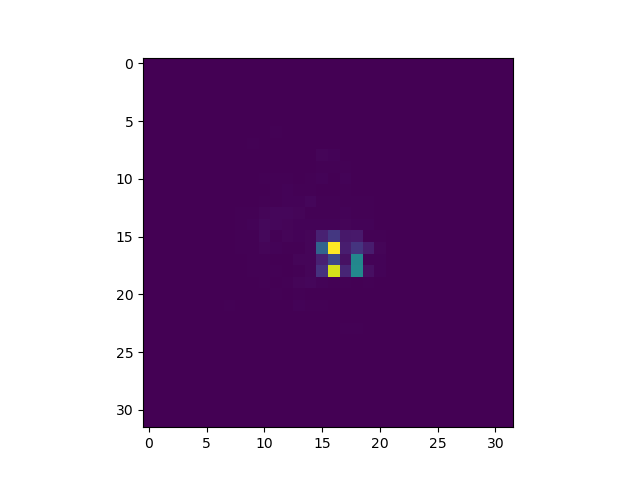
\includegraphics[width=.7\linewidth]{1450_poison_lrp.png}
			%\caption{Zugehörige Heatmap bezüglich der Klasse 'Höchstgeschwindigkeit: 80km/h'}
			
		\end{subfigure}
		\caption[(Optischer) Vergleich von korrumpiertem Datenpunkt und berechnter Heatmap.]{(Optischer) Vergleich von korrumpiertem Datenpunkt und berechnter Heatmap. Links: Verkehrsschild der Klasse 'Höchstgeschwindigkeit: 50km/h' versehen mit einem 3x3 Sticker und dem Label 'Höchstgeschwindigkeit: 80km/h'. Rechts: Zugehörige Heatmap bezüglich der Klasse 'Höchstgeschwindigkeit: 80km/h'.}
		\source{\cite{AC}}
		
		\label{vergleich_original_lrp}
	\end{figure}
	\subsection{Implementierungen}
	
	\subsubsection{Tensorflow}
	\subsubsection{pytorch}
	
	\textbf{Allgemeines Tutorial}:\footnote{\url{https://git.tu-berlin.de/gmontavon/lrp-tutorial}}\\ pytorch-LRP für VGG16 wird vorgestellt.\\
	
	
	\noindent \textbf{GiorgioML}\footnote{\url{https://giorgiomorales.github.io/Layer-wise-Relevance-Propagation-in-Pytorch/}}:\\
	Alternative pytorch-Implementierung basierend auf Tensorflow paper.\\
	
	\noindent \textbf{moboehle}\footnote{\url{https://github.com/moboehle/Pytorch-LRP}}:\\
	Der code entstand im Rahmen der Forschungsarbeit \cite{lrp_alzheimer}, in der eine Alzheimer-Festellung aufgrund von Bilddaten(scans?) vorgenommen wird. Framework leicht anpasspar. Benutzt pytorch hooks. 
	\noindent Unterstützte Netzwerkschickten\footnote{\url{https://github.com/moboehle/Pytorch-LRP/blob/master/inverter_util.py}}:\\
	\begin{comment}
	
	
	\noindent $allowed\_pass\_layers = (torch.nn.BatchNorm1d, torch.nn.BatchNorm2d,\\
	torch.nn.BatchNorm3d,
	torch.nn.ReLU, torch.nn.ELU, Flatten,
	torch.nn.Dropout,\\ torch.nn.Dropout2d,
	torch.nn.Dropout3d,
	torch.nn.Softmax,
	torch.nn.LogSoftmax,
	torch.nn.Sigmoid)$\\
	\end{comment}
	\begin{lstlisting}[language=Python, caption=Verfügbare Schichten und Aktivierungsfunktionen]
	torch.nn.BatchNorm1d, 
	torch.nn.BatchNorm2d
	torch.nn.BatchNorm3d,
	torch.nn.ReLU, 
	torch.nn.ELU, 
	Flatten,
	torch.nn.Dropout,
	torch.nn.Dropout2d,
	torch.nn.Dropout3d,
	torch.nn.Softmax,
	torch.nn.LogSoftmax,
	torch.nn.Sigmoid
	
	\end{lstlisting}
	\noindent \textbf{fhvilshoj}\footnote{\url{https://github.com/fhvilshoj/TorchLRP}}:\\
	
	
	
	\noindent LRP für linear und Convolutional layers
	
	\begin{itemize}
		\item Die Klassen
		
		torch.nn.Sequential, torch.nn.Linear und torch.nn.Conv2d werden erweitert, um autograd für die Berechnung der Relevanzen zu berechnen.
		
		\item Ausgabe der Relevanzen von Zwischenschichten ist möglich
		\item: Implementierte Regeln: epsilon Regeln mit epsilon=1e-1, gamma-regel mit gamma=1e-1. alphabeta-Reagel mit a1b0 und a2b1
		\item Netz muss hier umgeschrieben werden, sodass die Anwendung des Algorithmus möglich wird.
	\end{itemize}
	
	\begin{lstlisting}[language=Python, caption=Implementierte Regeln fhvilshoj]
	
	conv2d = {
	"gradient":             F.conv2d,
	"epsilon":              Conv2DEpsilon.apply,
	"gamma":                Conv2DGamma.apply,
	"gamma+epsilon":        Conv2DGammaEpsilon.apply,
	"alpha1beta0":          Conv2DAlpha1Beta0.apply,
	"alpha2beta1":          Conv2DAlpha2Beta1.apply,
	"patternattribution":   Conv2DPatternAttribution.apply,
	"patternnet":           Conv2DPatternNet.apply,
	}
	
	\end{lstlisting}
	
	\noindent \textbf{Zennit}:\footnote{\url{https://github.com/chr5tphr/zennit}}
	Zennit (Zennit explains neural networks in torch) 
	\begin{itemize}
		\item Modell wird mithilfe eines Canonizers so aufbereitet, dass LRP möglich wird
		\item Backward pass wird modifiziert, um Heatmaps zu erhalten.
		\item VGG- und ResNet-Beispiel
	\end{itemize}
	\section{Detektion von Poisoning-Angriffen basierend auf LRP} \label{chapter_algorithm}
	
	Super Einführung in Wasserstein und OT: \cite{altschuler2017near}\\
	Computing distances between probability measures on metric spaces, or more
	generally between point clouds, plays an increasingly preponderant role in ma-
	chine learning [SL11, MJ15, LG15, JSCG16, ACB17], statistics [FCCR16, PZ16,
	SR04, BGKL17] and computer vision [RTG00, BvdPPH11, SdGP+15]. A promi-
	nent example of such distances is the earth mover’s distance introduced in [WPR85]
	(see also [RTG00]), which is a special case of Wasserstein distance, or optimal
	transport (OT) distance [Vil09].
	While OT distances exhibit a unique ability to capture geometric features of
	the objects at hand, they suffer from a heavy computational cost that had been
	prohibitive in large scale applications until the recent introduction to the ma-
	chine learning community of Sinkhorn Distances by Cuturi [Cut13]. Combined
	with other numerical tricks, these recent advances have enabled the treatment
	of large point clouds in computer graphics such as triangle meshes [SdGP+15]
	and high-resolution neuroimaging data [GPC15]. Sinkhorn Distances rely on the
	idea of entropic penalization, which has been implemented in similar problems
	at least since Schrdinger [Sch31, Leo14]. This powerful idea has been success-
	fully applied to a variety of contexts not only as a statistical tool for model
	
	
	How Well Do WGANs Estimate the
	Wasserstein Metric? \cite{mallasto2019well}
	\subsection{Idee}
	Die Idee zur Detektion von Poisoning-Angriffen besteht aus den folgenden Schritten:
	
	\begin{itemize}
		\item Berechnung der Heatmaps mit Hilfe der LRP
		\item Berechnung einer Distanzmatrix basierend auf $L^2-$ oder GMW-Distanz
		\item Spektrale Relevanzanalyse (Bestimmung der verschiedenen Cluster innerhalb einer Klasse)
	\end{itemize}
	
	\noindent  \textbf{Bemerkung:} Anstatt das Clustering nur auf den Heatmaps durchzuführen, könnten die LRP-Ausgaben und/oder Aktivierungen bestimmer NEtzwerkschichten hinzugenommen werden.\\
	
	The theory of optimal transport generalizes thatintuition in the case where, instead of moving only one item at a time, one is concernedwith the problem of moving simultaneously several items (or a continuous distributionthereof) from one configuration onto another.\cite{computationalOT}
	\subsection{k-means / k-means++ -Clustering}
	
	Beispiel-Implementierung\footnote{\url{https://towardsdatascience.com/k-means-implementation-in-python-and-spark-856e7eb5fe9b}}\\
	\\
	Baryzentrische Koordinaten \footnote{\url{https://de.wikipedia.org/wiki/Baryzentrische_Koordinaten}}
	
	\subsection{Spektrales Clustering}
	Wir folgen \cite{spectralClustering_tut}.
	Gegeben:Datenpunkte $x_i, ..., x_n$ sowie eine Größe $s = s_{ij} \in \mathbb{R}^{+}$, die einen paarweisen Zusammenhang der einzelnen Punkte beschreiben.
	
	Ziel: Aufteilen der Punkte in verschiedene Cluster, sodass sich Punkte innerhalb eines Clusters ähnlich bezüglich $s$ sind.
	
	Alternative Repräsentation der Daten mithilfe eines Ähnlichkeitsgraphen $G=(V,E)$ möglich.
	
	Umformulierung des Clustering-Problems mithilfe des Ähnlichkeitsgraphen: Finde Pertitionierung des Graphen, sodass die Kanten-Gewichte innerhalb einer Gruppe niedrig (niedriges Gesamtgewicht?) und außerhalb einer Gruppe große sind.\\
	
	
	Graph-Notationen:\\
	
	Verschiedene Konstruktionsmöglichkeiten von Ähnlichkeitsgraphen:
	
	\begin{itemize}
		\item $\varepsilon$-Nachbarschaft-Graph\\
		\item kNN-Graph\\
		\item fully connected graph
	\end{itemize}
	
	
	\subsection{Anwendung auf unterschiedliche Poisoning-Angriffe} \label{chapter_results} \label{chapter_experiments}
	\noindent \textbf{Berechnung der Relevanzen}:\\
	
	\noindent Wir berechnen die Relevanzen jedes einzelenen Eingabebildes klassenweise, d.h. besitzt eine Eingabe das Label y, so berechnen auf einem trainierten Netzwerk, für jeden Pixelwert der Eingabe, wie relevant dieser für die Ausgabe f(x) = y ist.\\
	Wir summieren über die Farbaxen des Bildes, um einzelne Relevanzen pro Pixelpunkt zu erhalten.\\
	Für die Berechnung der Relevanzen benutzen wir eine modifizierte Version des im Rahmen von \cite{lrp_alzheimer} entstandenen Programmcodes\footnote{\url{https://github.com/moboehle/Pytorch-LRP}}.\\
	\\
	\noindent \textbf{Vorverarbeitung der Relevanzen:}\\
	In \cite{unmaskingCH} wird anschließend ein Sum-Pooling auf die Relevanzen angewendet, um eine Dimensionsreduktion zu erhalten. Wie in \cite{imagenet_unhansed_v1} verzichten wir auf eine weitere Dimensionsreduktion, da wir nur relativ kleine Relevanzen der Größe $32x32$ verarbeiten.	\\
	
	Für eps=5e-2 liegen beide barycentren identisch weit weg. Probiere nun eps=5e-3
	
	\noindent \textbf{Berechnung der Distanzen und Aufstellen einer Affinitätsmatrix:}\\
	
	Wir berechnen zunächst eine Distannzmatrix, die die paarweisen Distanzen aller Heatmaps einer Klasse enthält.	
	
	Für die Berechnung der euklidischen Distanz betrachten wir Heatmaps $x,y$ der Größe $32x32$ als Elemente $x,y \in \mathbb{R}^{32*32}$ Die Distanz lässt sich dann wie in \autoref{l2dist} berechnen.\\
	
	Die Gromov-Wasserstein-Distanz lässt sich wie in \cite{gwd_averaging_kernels} angegeben berechnen. \\
	
	Barycenters Definition und Vergleich zum euklidischen Raum \cite{bary_wasserstein_space}
	
	In einer Affinitätsmatrix oder Ähnlichkeitsmatrik sind die \\
	
	\noindent \textbf{Berechnung Spektralen Einbettung:}\\
	
	\noindent \textbf{Dimensionsreduktion vor dem Clustering ?!}\\
	
	In \cite{AC} wird beispielsweise eine Dimensionsreduktion mit PCA durchgeführt.
	
	\noindent \textbf{k-Means-Clustering:}\\
	\begin{remark}
		In \cite{imagenet_unhansed_v1} Kapitel '2.3. Fisher Discriminant Analysis for Clever Hans
		identification' wird ein Verfahren vorgestellt, mit dem verdächtige Klassen indentifiziert werden können. Für diese würde man anschließend das obige Verfahren durchführen
	\end{remark}
	\subsection{Verwendete Distanzen \& Approximationen}
	Um die Struktur innerhalb einer Klasse zu analysieren, benötigen wir eine Metrik.
	Anhand dieser wird abhängig von den Heatmps einer Klasse eine Affinitätsmatrix berechnet, die dann anschließend zur Berechnung der Spektralen Einbettung als wichtigster Schritt von SpRAy verwendet wird. Wir wollen dazu die im Folgenden vorgestellten Metriken verwenden.\\
	Wie in \cite{imagenet_unhansed_v1} summieren wir über die Farbkanäle, um einen einzelnen Relevanzwert pro Pixelpunkt zu erhalten. Wir benötigen also eine Metrik zur Berechnung der Distanz zwischen 32x32 großen Heatmaps.\\
	Wir normalisieren die Relevanzen zusätzlich auf das Intervall $[0,1]$.\\
	Die Wahl der Pixel mit 99 Prozent der Gesamtmasse und anschließende Normalisierung wird vermutlich durchgeführt, um die Bedingung \autoref{eq:bed_mmspaces} zu erhalten.
	\section{Optimal Transport}
	
	Optimal Transport is an interesting topic which connects many fields and has
	interesting applications
	Applications in image analysis
	Interplay between geometry, probability and PDEs
	Convexity, duality
	Numerical optimization
	Statistics and Machine Learning\footnote{\url{https://indico.cern.ch/event/845380/attachments/1915103/3241592/Dvurechensky_lectures.pdf}}
	
	Optimal transport can deal with smooth and discrete measures and it has proved to be very useful
	for comparing distributions in a shared space, but with different (and even non-overlapping) supports\cite{vayer2020fused}.
	Einführung OT Villani%\footnote{\url{https://books.google.de/books?hl=en&lr=&id=idyFAwAAQBAJ&oi=fnd&pg=PR11&dq=villani+2003&ots=YRvDCQXIIn&sig=XqyOf4Qqsw-otlBm0_4L3YoU6pA&redir_esc=y#v=onepage&q=villani\%202003&f=false}}
	OT hebt Distanzen von metrischen Räumen auf den Raum der metrischen Räume \cite{memoli2011gromov}.
	
	In diesem Kapitel betrachten wir einige Konzepte aus dem Bereich Optimal Transport, um einen Distanzbegriff zu entwickeln, der im Unterschied zur pixel-weisen euklidischen Distanz besser für das kMeans-Clustering geeignet sein könnte.
	Ausgehend von Gaspard Monge's ursprünglicher Transportproblme-Formulierung betrachten wir die durch Kantorobich eingeführte Relaxierung dieses Problems.
	Die Optimale Lösung wird für die Definition der p-Wasserstein-Distanz verwendet.
	Für eine Verallgemeinerung auf verschiedene Grundräume wird die Gromov-Wasserstein-Distanz definiert. Damit können wir zwei Heatmaps als sogenannte metrische Maßräume auffassen.
	Abschließend definieren wir sogenannte Gromov-Wasserstein-Baryzentren, die im Rahmen des kMeans-Clustering als Mittelwerte fungieren.
	
	Stimmt Gromov-Wassertsien mit Wsserstein für dieselbe Distanfunktion(Metrik) überein? Welche Rolle spielt die Lossfunktion L bei der Definition? Ja, siehe Memoli 2011.
	L=KL
	\subsection{Einführung}
	\subsubsection{Frage:}
	Was ist ein registration problem?
	Warum brauchen wir Gromov-Wasserstein? Warum reicht nicht Wasserstein? Weil wir Matrizen unterschiedlicher Größer vergleichen? Nein. Wir benutzen ja immer dieselbe Distanz für alle Pixel-Werte.
	Wenn wir eine Pixel-Wolke auswählen, sind das nicht dieselben Räume, da dann gewisse Koordinaten nicht zum Raum gehören. Wenn wir aber alle Pixel als Koordinaten im Raum auswählen würden, dann würden die metrischen Räume $(X,d_X)$ und $(Y,d_Y)$ übereinstimmen. Liegt das an der Definition der Baryzentren? Wie würde man das mit Baryzentren auf demselben Raum machen? s. \cite{COTcuturi}
	Translationen und Rotationen könnte ein wichtiger Punkt sein!!!
	verwendung von Grafiken aus anderen Papern??
	Kann man ein anderes Netzwerk zur Detektion nutzen?
	
	\url{https://arxiv.org/pdf/1705.09634.pdf}
	\url{https://arxiv.org/pdf/1412.5154.pdf}
	Für die Grudnlagen im Bereich des Optimalen Transports zitieren wir \cite villani2009optimal.
	
	Entscheidend für die Numerischen Resultate ist die Arbeit von Marco Cuturi \cite{cuturi2013sinkhorn, computationalOT}
	
	\cite{COTcuturi} Remark 2.19 (Translations). zeigt dass die Unabhängigkeit gegenüber Translationen? Kann ich das auch für die Gromov-Wasserstein-Distanz zeigen?
	\subsubsection{Anwendungsgebiete}
	Optimal transport is also used widely in domain adaptation \cite{courty2016optimal}. In domain adaptation, one has
	access to labeled examples from a source domain and unlabeled examples from a target domain.
	The goal is to predict labels for examples from the target domain. This is different from the typical
	train-test paradigm in machine learning, because covariate shift between the two domains is allowed.
	
	
	Ein weitere Anwendung von Optimal Transport sind Wasserstein Generative Adversarial Networks (WGANs) \cite{wgan}. WGANs gehören zur Familie der Modelle namens Generative Adversarial Networks (GANs) \cite{gan}. Zu einem GAN gehören zwei Modelle, von denen beide typischerweise Neuronale Netzwerke sind. Das erste Netzwerk (generator) erzeugt Datenpunkte innerhalb des Datensatzes, die so realsitisch wie möglich sein sollen. Das zweite Netzwerk (discriminator network) versucht, zwischen den realen und den erzeugten Datenpunkten zu unterscheiden. Damit kann der Trainingsprozess von GANs als ein Spiel zwischen den beiden Netzwerken betrachtet werden, bei dem der Generator den Diskriminator täuschen und der Diskriminator die korrumpierten Datenpunkte aufdecken möchte.
	
	Durch die Verwendung von WGANs ansatts GANs wurde ein stabilerer Trainingsprozess erreicht, da diese weniger anfällig für abrupte Trainingsabbrüche sind. Die ursprünglichen GANs benutzten eine Jensen-Shannon-Divergenz als Verlustfunktion, die nicht überall stetig und fast überall differenzierbar ist. Auch andere Verlustfunktion wie besipielsweise die KL-Divergenz weisen ähnliche Schwierigkeiten auf. Durch die Verwendung der Wasserstein-Verlustfunktion, basierend auf der 1-Wasserstein-Distanz, die überall stetig und fast überall differenzierbar ist, konnte der Trainingsprozess der GANs somit deutlich verbessert werden \cite{mauryaoptimal}.
	
	
	
	\begin{definition}
		
	\end{definition}
	
	\begin{definition}[Histogramm]
		Als Histogramm (oder: Wahrscheinlichkeitsvektor) bezeichnen wir ein Element $\boldsymbol{a} \in \Sigma_n$, das zum folgenden Wahrscheinlichkeits-Simplex gehört:
		
		\begin{equation*}
		\Sigma_n := \lbrace \boldsymbol{a} \in \mathbb{R}_{+}^n | \sum_{i=1}^n{\boldsymbol{a_i} = 1} \rbrace
		\end{equation*}
	\end{definition}


\begin{definition}[\cite{gromov2007metric}]
	Ein metrischer Maßraum ist ein Tripel $(X, d_X, \mu_X)$ mit
	\begin{itemize}
		\item $(X, d_X)$ ist ein kompakter metrischer Raum
		\item $\mu_X$ ist ein Borel-Maß auf $X$ mit vollem Support, d.h. 
		\begin{equation}
			supp[\mu_X] = X.\label{eq:bed_mmspaces}
		\end{equation} 
	\end{itemize}

\begin{definition}[pushforward-Maß]
	Seien $X,Y$ zwei Maßräume, $T: X \to Y$ eine messbare Abbildung und $\mu$ ein Maß auf X. Dann ist das pushforwad-Maß $T^\# \mu $ ein Maß auf Y, definiert durch \begin{equation}
	T^\# \mu (A) = \mu (T^{-1}(A))
	\end{equation}
	für alle $A \subset Y$.
\end{definition}
	
\end{definition}
	
	Einführung W-Theorie am KIT \footnote{\url{https://www.math.kit.edu/stoch/~henze/media/wt-ss15-henze-handout.pdf}}
	\begin{definition}[Kopplungen zwischen Histogrammen]
		Seien die beiden Histogramme $p \in \Sigma_{N_1}$ und $q \in \Sigma_{N_2}$ gegeben.
		Als Menge der Kopplungen zwischen beiden Histogrammen definieren wir
		
		\begin{equation*}
		\mathcal{C}_{p,q} := \lbrace T \in (\mathbb{R}_+)^{N_1 \times N_2} | T \mathbb{1}_{N_2} = p, T^\top \mathbb{1}_{n_1} = q \rbrace,
		\end{equation*}	
		
		wobei $\mathbb{1} := (1,...,1)^\top \in \mathbb{R}^{N}$ gilt.
	\end{definition}
	
	

	\begin{definition}[\cite{burago2001course}]
		Sei $X$ eine beliebige Menge. Eine Funktion $d:X \times X \to \mathbb{R} \cup \lbrace \infty \rbrace$ heißt \emph{Metrik} auf $X$, falls die folgenden Bedingungen für alle $x,y,z \in X$ gelten:
		\begin{enumerate}[label={(\arabic*)}]
			\item Positive Definitheit: $d(x,y) > 0 \text{ für } x \neq y \text{ und } d(x,y)=0 \text{ für } x=y$,
			\item Symmetrie: $d(x,y)=d(y,x)$,
			\item Dreiecksungleichung: $d(x,z) \leq d(x,y) + d(y,z)$.	
		\end{enumerate}
	\end{definition}
	Ein \emph{metrischer Raum} ist eine Menge, versehen mit einer Metrik. Formal gesehen ist ein metrischer Raum ein Paar $(X,d)$, wobei $d$ eine Metrik auf $X$ ist. Elemente von $X$ heißen Punkte und $d(x,y)$ bezeichnet die Distanz zwischen $x$ und $y$.
	
	
	
	

	Geodesic Space \footnote{\url{http://www.math.toronto.edu/mccann/papers/FiveLectures.pdf}}
	
	\noindent \textbf{Gromov-Hausdorff-Distanz}
	
	\begin{definition}[Hausdorff-Distanz]
		Sei $(M,d)$ ein metrischer Raum.
		Für 
		Seien $X,Y \subset (M,d)$ definieren wir die \emph{Hausdorff-Distanz} $d_H(X,Y)$ als
		
		\begin{equation}
		d_H(X,Y) = \max \lbrace \sup_{x \in X} \inf_{y \in Y} d(x,y), \sup_{y \in Y} \inf_{x \in Y} d(x,y) \rbrace .
		\end{equation} 
		
	\end{definition}
	
	%\begin{figure}
	%	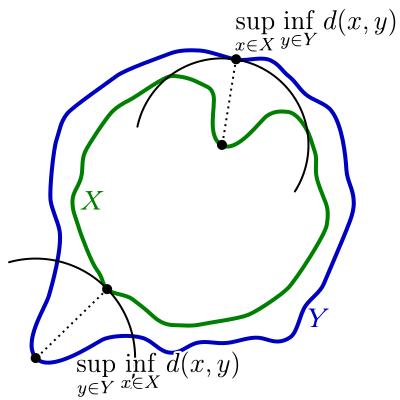
\includegraphics{Hausdorff_distance_sample}
	%\end{figure}
	\begin{definition}[Metrischer Maßraum]
		Ein \emph{metrischer Maßraum} ist ein Tripel $(X,d_x,\mu_X)$, wobei $(X,d_X)$ ein metrischer Raum und $\mu_X$ ein borelsches W-Maß auf $X$ ist.
	\end{definition}
	
	\begin{definition}[Correspondance]
		content...
	\end{definition}
	
	\begin{definition}[Kopplung]
		Seien 
	\end{definition}
	
	Seien $(X,d_X)$ und $(Y,d_Y)$ zwei metrische Räume. Wir betrachten im Folgenden die Abbildung
	\begin{equation}
	\Gamma_{X,Y}: (X\times Y) \times (X \times Y) \to \mathbb{R^{+}},
	\end{equation}
	gegeben durch
	
	$\Gamma_{X,Y}(x,y,x',y'):= |d_X(x,x') - d_Y(y,y')|$.
	
	\begin{definition}[Gromov-Hausdorff-Distanz]
		Für die metrischen Räume $(X,d_X)$ und $(Y,d_Y)$ ist die \emph{Gromov-Hausdorff-Distanz} definiert als
		\begin{equation}
		d_{\mathcal{G}\mathcal{H}} = \frac{1}{2}\inf_{R}||\Gamma_{X,Y}||_{L^\infty(R \times R)}.
		\end{equation}
	\end{definition}
	\begin{definition}[Entropischer Optimaler Transport]
		Wir definieren den $n$-dimensionalen Zufalls-Simplex als $\Sigma_n := \lbrace a \in \mathbb{R}_+^n: \sum_{i=1}^{n}{a_1} = 1$. Ein Element $a \in \Sigma_n$ bezeichnen wir als Histogramm oder Zufallsvektor.
		
	\end{definition}
	
	\begin{definition}[Diskretes Maß]
		
	\end{definition}

	\subsection{Kantorovichs Optimal Transport}
	\subsubsection{Optimaler Transport (Monge Formulierung)}
	\begin{remark}
		Problem zwischen diskreten Maßen
		
		\begin{equation}
		\min_T \lbrace \sum_i {c(x_i, T(x_i))} : T_\#\alpha = \beta \rbrace
		\end{equation}
	\end{remark}
	\begin{remark}[Fehlende Eindeutigkeit]
		
	\end{remark}
	
	\begin{definition}[Push-forward Operator]
		$\beta (B) = \alpha (\lbrace x \in \mathcal{X}: T(x) \in B \rbrace) = \alpha(T^{-1}(B))$ \label{eq_pushforward}
		
	\end{definition}
	Wir könne das Monge Problem wie folgt auf den Fall zweier beliebiger W-Maße $(\alpha, \beta )$ erweitern.
	
	\begin{definition}[Monge Problem zwischen beliebigen Maßen]
		Seien $\alpha$ und $ \beta$ zwei W-Maße mit Support auf den Räumen $\mathcal{X}$ bzw. $\mathcal{Y}$, die durch $T:\mathcal{X} \to 	\mathcal{Y}$ verknüpft(? Fomulierung) sind.
		Dann ist das Monge Problem gegeben durch
		\begin{equation}
		\min_T \lbrace \int_\mathcal{X}{c(x,T(x)) d\alpha (x)} : T_\#\alpha = \beta \rbrace.
		\end{equation}
	\end{definition}
	Die Bedingung $T_\#\alpha = \beta$ bedeutet, dass die Abbildung $T$ die gesamte Masse mithilfe des Push-forward Operators von $\alpha$ auf $\beta$ schiebt.
	\subsubsection{Optimaler Transport nach Kantorovich}
	\cite{santambrogio2010introduction} ist eine gute, einfache Einführung. Damit kann ich vermutlich Monge und Kantorovich beschreiben.
	
	Das Optimal Transport Problem nach Kantorovich gehört zu den typischen Optimal Transport Problemen. Es stellt einer Relaxierung der Formulierung von Gaspard Monge[1781], bei der nun auch das Aufteilen von Masse (mass splitting) zulässig ist.
	In Kantorovichs Formulierung ist eine Kopplung (oder: Transportabblidung) $\boldsymbol{T}$ gesucht, die die Kosten, die bei der Verschiebung eines diskreten Maßes $\boldsymbol{a}$ auf ein anderes diskretes Maß $\boldsymbol{b}$ bezüglich der Kosten $\boldsymbol{M} \in \mathbb{R}^{n_1 \times n_2}$ entstehen, minimiert.
	Damit $\boldsymbol{T}$ eine Transportabbildung ist, muss $\boldsymbol{T} \in \Gamma(a,b) = \lbrace \boldsymbol{T} \geq \boldsymbol{0}, \boldsymbol{T}\boldsymbol{1}_{n_2} = a, \boldsymbol{T}^{T}\boldsymbol{1}_{n_1} = \boldsymbol{b} \rbrace$ gelten.
	
	Für den Fall, dass die Grundkosten eine Metrik darstellen, ist auch die optimale Lösung des Optimal Transport Problems wieder eine Metrik \cite{cuturi2014ground} und definiert die \textit{Wasserstein Distanz}. Das OT Problem ist definiert als
	\begin{equation}
	W_M(\boldsymbol{a},\boldsymbol{b}) = \min_{T \in \Pi(\boldsymbol{a}, \boldsymbol{b})}{\langle \boldsymbol{T}, \boldsymbol{M} \rangle},
	\end{equation}
	
	wobei ${\langle \boldsymbol{T}, \boldsymbol{M} \rangle} = \sum_{ij}{t_{ij}m_{ij}}$ gilt.
	
	Die Lösung des Problems ist eine Kopplung/Kopplungsmatrix, die beschreibt, wie viel Masse von einem Punkt zum anderen Punkt fließt. In einer Kostenmatrix derselne Größe sind die Kosten abgespeichert, um von einem zum anderen Punkt zu kommen.
	
	which is a linear program. The optimization problem above is often adapted to include a
	regularization term for the transport plan T , such as entropic regularization (Cuturi, 2013)
	or squared L2. For the entropic regularized OT problem, one may use the Sinkhorn Knopp
	algorithm (or variants), or stochastic optimization algorithms. POT has a simple syntax to
	solve these problems (see Sample 1)
	
	Die Menge der Matrizen $\Pi(\boldsymbol{a}, \boldsymbol{b})$ ist beschränkt und durch $n+m$ Gleichungen gegeben und damit ein konvexes Polytop (die konvexe Hülle einer endlichen Menge von Matrizen). Zudem ist die Formulierung von Kantorovich im Unterschied zu Monges Formulierung immer symmetrisch in dem Sinne, dass $\boldsymbol{P} \in \Pi (\boldsymbol{a}, \boldsymbol{b})$ genau dann gilt, wenn $\boldsymbol{P}^\top \in \Pi (\boldsymbol{b}, \boldsymbol{a})$.
	
	Kantorovichs Optimal Transport Problem lässt sich nun schreiben als 
	\begin{equation}
	L_C(\boldsymbol{a}, \boldsymbol{b}) := \min_{P \in \Pi(\boldsymbol{a}, \boldsymbol{b})} \langle \boldsymbol{C}, \boldsymbol{P} \rangle := \sum_{i,j}{\boldsymbol{C}_{i,j}\boldsymbol{P}_{i,j}} \label{KOTP}
	\end{equation}
	
	Diese Problem ist ein lineares Problem. Für diese Art von Problemen ist die optimale Lösung nicht notwendigerweise eindeutig. In fact Kantorovich is considered as the inventor of linear pro-
	gramming. \footnote{OTNotes\_campride.pdf}
	
	EXISTENZ \& Eindeutigkeit => vgl. Kapitel 3 in \cite{computationalOT}
	
	
	
	\begin{definition}[Formulierung für beliebige Maße]
		Im Fall beliebiger Maße betrachten wir die Kopplungen $\pi \in \mathcal{M}_+^1(\mathcal{X} \times \mathcal{Y})$, die die gemeinsame Verteilung auf dem Produktraum $\mathcal{X} \times \mathcal{Y}$ ist. Im diskreten Fall verlangen wir, dass das Produktmaß die Form $ \pi = \sum_{i,j}{\boldsymbol{P}_{i,j}\delta_{(x_i, y_j)}}$ besitzt. Im Allgemeinen Fall wird die Massenerhaltung als Randbedingung an die gemeinsame W-Verteilung geschrieben:
		
		\begin{equation}
		\Pi(\alpha, \beta) := \lbrace \pi \in \mathcal{M}_+^1(\mathcal{X} \times \mathcal{Y}): P_{\mathcal{X}_\#} \pi = \alpha \text{ und } P_{\mathcal{Y}_\#} \pi = \beta \rbrace,
		\end{equation}
		wobei $P_{\mathcal{X}_\#}$ und $P_{\mathcal{Y}_\#}$ die Push-forward Operatoren der Projektionen $P_\mathcal{X}(x,y) = x$ und $P_\mathcal{Y}(x,y) = y$ sind. Nach \autoref{eq_pushforward} sind diese Randbedingungen äquivalent zu den Bedingungen $\pi(A \times \mathcal{Y}) = \alpha (A)$ und $\pi (\mathcal{X} \times B) = \beta (B)$ für die Mengen $A \subset \mathcal{X}$ und $B \subset \mathcal{Y}$.
		Als Verallgemeinerung erhalten wir dann
		\begin{equation}
		\min_{\pi \in \Pi (\alpha, \beta)}\int_{\mathcal{X} \times \mathcal{Y}}{c(x,y) d\pi (x,y)}. \label{eq:kontorovich_allgemein}
		\end{equation}
	\end{definition}
	
	Problem \autoref{eq_kontorovich_allgemein} ist ein unendlich-dimensionales lineares Programm über einem Raum von Maßen. Falls $(\mathcal{X}, \mathcal{Y})$ kompakt und $c$ stetig ist, existiert immer eine Lösung.
	
	\begin{example}
		Beispiele von Kopplungen
	\end{example} 
	\subsubsection{Monge-Kantorovitch equivalence}
	The proof of Brenier theorem 1 (detailed in Section 5.3) to prove
	the existence of a Monge map actually studies Kantorovitch relaxation, and proves that this relaxation is
	tight in the sense that it has the same cost as Monge problem.\footnote{CourseOT\_cuturi}
	\subsubsection{Metrische Eigenschaften}
	Optimaler Transport definiert eine Distanz zwischen Histogrammen und W-Maßen, sofern die Kostenmatrix gewisse Eigenschaften erfüllt. Optimal Transport kann dabei als naheliegende Idee verstanden werden, um Distanzen zwischen Punkten auf Distanzen zwischen Histogrammen oder Maßen zu verallgemeinern.
	
	\begin{definition}[p-Wasserstein-Distanz auf $\Sigma_n$]
		Sei $n=m$ und für $p \geq$ gelte $\boldsymbol{C} = \boldsymbol{D}^p = (\boldsymbol{D}_{i,j}^p)_{i,j} \in \mathbb{R}^{n \times n}$, wobei $\boldsymbol{D} \in \mathbb{R}_+^{n \times n}$ eine Metrik ist.
		
		Dann definiert 
		\begin{equation}
		W_p(\boldsymbol{a}, \boldsymbol{b}) := L_{\boldsymbol{D}^p} (\boldsymbol{a}, \boldsymbol{b})^{1/p}
		\end{equation} 
		die $p$-Wasserstein-Distanz auf $\Sigma_n$
	\end{definition}
	
	\begin{lemma}
		$W_p$ ist eine Metrik
	\end{lemma}
	
	\begin{proof}
		Nach Voraussetzung besitzt $\mathcal{C} = \mathcal{D}^p$ eine Nulldiagonale. Somit gilt $W_p(\boldsymbol{a},\boldsymbol{a}) =0.$. Die zugehörige Transportmatrix ist $\boldsymbol{P}^\star = diag(\boldsymbol{a})$. Aufgrund der Positivität aller Nicht-Diagonalelemente von $\boldsymbol{D}^p$ gilt $W(\boldsymbol{a},\boldsymbol{b})$ für $\boldsymbol{a} \neq \boldsymbol{b}$, da in disem Fall jede zulässige Kopplungen und damit insbesonder die optimale Kopplungen ein Nicht-Diagonalelemnt ungleich $0$ besitzt. Die Symmetrie von $W_p(\boldsymbol{a},\boldsymbol{b})$ gilt wegen der Symmetrie von $\boldsymbol{D}^p$.
		
	 	Für den Nachweis der Dreiecksungleichung im Fall beliebiger Maße nutzt Villani \cite{villani2003topics} das sogenannte Gluing Lemma. Im diskreten Fall ist die Konstruktion dieser geklebten Kopplung etwas einfacher. Seien $\boldsymbol{a}, \boldsymbol{b}, \boldsymbol{c} \in \Sigma_n$. Seien $\boldsymbol{P}$ und $\boldsymbol{Q}$ zwei optimale Lösungen des Transportproblems zwischen $\boldsymbol{a}$ und $\boldsymbol{b}$ bzw. $\boldsymbol{b}$ und $\boldsymbol{c}$.
	 	Wir definieren $\tilde{\boldsymbol{b}}$, wobei $\tilde{\boldsymbol{b}}_j = \boldsymbol{b}_j$, falls $\boldsymbol{b}_j > 0$, und $\tilde{\boldsymbol{b}}_j = 1$ sonst gilt. Damit können wir 
	 	\begin{equation}
	 		\boldsymbol{S}:= \boldsymbol{P} diag(1/\tilde{\boldsymbol{b}})\boldsymbol{Q} \in \mathbb{R}_+^{n\times n}
	 	\end{equation}
	 	schreiben. Es gilt $\boldsymbol{S} \in \Pi (\boldsymbol{a}, \boldsymbol{c})$ wegen
	 	\begin{equation}
	 	\boldsymbol{S}\boldsymbol{1}_n = \boldsymbol{P} diag(1/\tilde{\boldsymbol{b}})\boldsymbol{Q}\boldsymbol{1}_n = \boldsymbol{P}(\boldsymbol{b}/\tilde{\boldsymbol{b}}) = \boldsymbol{P}\boldsymbol{1}_{supp[\boldsymbol{b}]} = \boldsymbol{a},	 	\end{equation}
	 	wobei $\boldsymbol{1}_{supp[\boldsymbol{b}]}$ den Vektor der Größe $n$ bezeichnet, der Einsen an den Stellen mit Indizes $j$ besitzt, für die auch $\boldsymbol{b}_j >0$ gilt, und sonst aus Nullen besteht.
	 	Außerdem wurde $\boldsymbol{P}\boldsymbol{1}_{supp[\boldsymbol{b}]} = \boldsymbol{P}\boldsymbol{1}_n = \boldsymbol{a}$ benutzt, denn es gilt notwendigerweise $\boldsymbol{P}_{i,j} = 0$ für diejenigen $j$ mit $\boldsymbol{b}_j = 0$. Analog folgt $\boldsymbol{S}^\top\boldsymbol{1}_n = \boldsymbol{c}$.
	 	
	 	Damit erhalten wir
	 	
	 	\begin{align}
	 		content...
	 	\end{align}
	\end{proof}
	
	\begin{remark}[Der Fall $0 < p \leq 1$]
		Für $0 < p \leq 1$ ist auch $D^p$ eine Distanz. Damit ist für $ p \leq 1$ $W_p(\boldsymbol{a}, \boldsymbol{b})^p$ eine Distanz au dem Simplex.
		
	\end{remark}

\begin{remark}
	Für $p=1$ ist die p-Wasserstein-Distanz auch als Earth Movers's Distance \cite{rubner2000earth} bekannt
\end{remark}
	\subsubsection{Duale Formulierung}
	Kurzer Überblick hier\footnote{\url{https://arxiv.org/pdf/1609.04767.pdf}}
	oder (Herleitung der Dualen Formulierung mit Beweis)\footnote{\url{text}}.
	
	The Kantorovich problem (2.11) is a constrained convex minimization problem, and as
	such, it can be naturally paired with a so-called dual problem, which is a constrained
	concave maximization problem. The following fundamental proposition explains the
	relationship between the primal and dual problems.
	
	\subsubsection{Verfahren zur Berechnung der exakten Lösung}
	
	\subsubsection{Komplexitätsanalyse}
	Im Fall $n=m$ ist das Kantorovich-Problem und damit die Berechnung der Wasserstein-Distanz ein lineares Optimierungsproblem mit $\mathcal{O}(n)$ linearen Bedingungen. Für die Lösung kann beispielsweise der lineare Lee-Sinford-algorithmus zur Berechnung einer Lösung in $\tilde{\mathcal{O}}(n^{2.5})$ \cite{lee2014path} verwendet werden, der den vorherigen Standard von $\mathcal{O}(n^{2.5})$ \cite{renegar1988polynomial} verbessert.
	\subsubsection{Wasserstein-Baryzentren}
	
	\subsubsection{Andere Regularisierungen}
	Tradeoff zwischen numerischem Aufwand und statistischer Genauigkeit.
	
	Mehrere Möglichkeiten einer Regularisierung der GW-Distanz\footnote{\url{https://www.youtube.com/watch?v=cPVMHWF8fmE&t=2532s}}:
	\begin{itemize}
		\item Entropic regularization [Cuturi, 2013]\\
		\item Group Lasso [Courty et al., 2016a]\\
		\item KL, Itakura Saito, $\beta$-divergences,
		[Dessein et al., 2016]
	\end{itemize} 
	
	
	\subsection{Entropisch regularisierte Wasserstein-Distanz}
	In diesem Abschnitt betrachten wir regularisierte Version der Wasserstein-Distanz mithilfe von Entropie. 
	Diese von Marco Cuturi vorgestellte Regularisierung \cite{cuturi2013sinkhorn} verhalf dem Gebiet des Computational Optimal Transport zu sehr großem in Interesse. Durch die Regularisierung mit Entropie entsteht eine Kullback-Leibler-Distanz, für die Standard-Verfahren wie beispielsweise der Sinkhorn-Algorithmus verwendet werden können.
	Andere Arten der Regularisierung sind Group Lasso [Courty et al., 2016a] und KL, Itakura Saito, $\beta$-divergences,
	[Dessein et al., 2016].\footnote{\url{https://www.damtp.cam.ac.uk/research/cia/files/teaching/Optimal_Transport_Syllabus.pdf}}
	
 	Wir definieren die diskrete Entropie eine Kopplungsmatrix wie folgt.
 	
	\begin{definition}[Entropie]
		Für $T \in \mathbb{R}_{+}^{n \times n}$ definieren wir die Entropie als
		\begin{equation}
		H(T) := - \sum_{i,j=1}^N{T_{i,j}(log(T_{i,j})-1)}.
		\end{equation}
	\end{definition}
	Entropic Regularization of Optimal Transport \cite{computationalOT}
	
	
	Optimal Transport: Regularization and Applications
	\footnote{\url{https://www.otra2020.com/schedule}}
	Python Optimal Transport Toolbox\footnote{\url{https://pythonot.github.io/quickstart.html}}\footnote{\url{https://pythonot.github.io/auto_examples/gromov/plot_gromov.html}}
	
	Kapitel 2.1 im Paper: Vergleich von Histogrammen auf demselben metrischen Raum.
	
	\begin{lemma}
		$L_C(\boldsymbol{a}, \boldsymbol{b}):= \min_{P \in \Pi(\boldsymbol{a}, \boldsymbol{b})}{\langle \boldsymbol{P}, \boldsymbol{C} \rangle - \varepsilon \boldsymbol{H}(\boldsymbol{P})}$\label{eq:reg_problem}
		
		ist ein $\varepsilon$-streng konvexes Problem und besitzt deshalb eine eindeutige optimale Lösung
		test
	\end{lemma}
	
	\begin{proof}
		Die Entropie H ist wegen der Hesse-Matrix $\partial ^2 H (P) = -diag(1/P_{i,j})$ und $P_{i,j} \leq 1$ stark konkav.
		Durch die Multiplikation mit $\varepsilon$ und anschließender Subtraktion wir aus dem obigen Problem ein konvexes. 
	\end{proof}

	\begin{remark}
		Für größere $\varepsilon$ wird mehr Entropi gefordert
	\end{remark}
	
	\begin{proposition}[Konvergenz in $\varepsilon$]
		Die eindeutige Lösung $P_\varepsilon$ von \autoref{eq:reg_problem} konvergiert gegen die optimale Lösung mit maximaler Entropie innerhalb der Menge aller optimalen Lösungen des Kantorovich Problems, d.h.
		\begin{equation}
		\boldsymbol{P}_\varepsilon \xrightarrow{\varepsilon \to 0} \argmin_{P} \lbrace -\boldsymbol{H}(\boldsymbol{P}) : \boldsymbol{P} \in \Pi (\boldsymbol{a}, \boldsymbol{b}), \langle \boldsymbol{P}, \boldsymbol{C} \rangle = L_{\boldsymbol{C}}(\boldsymbol{a}, \boldsymbol{b}) \rbrace, \label{eq:P_eps_0} 
		\end{equation}
		d.h. es gilt
		\begin{equation}
		L_{\boldsymbol{C}}^\varepsilon (\boldsymbol{a}, \boldsymbol{b}) \xrightarrow{\varepsilon \to 0} L_{\boldsymbol{C}}(\boldsymbol{a}, \boldsymbol{b})
		\end{equation}
		Zudem gilt
		\begin{equation}
		\boldsymbol{P}_\varepsilon \xrightarrow{\varepsilon \to \infty} \boldsymbol{a} \otimes \boldsymbol{b} = \boldsymbol{a} \boldsymbol{b}^\top = (\boldsymbol{a}_i \boldsymbol{b}_j)_{i,j}. \label{eq:P_eps_infty}
		\end{equation}
	\end{proposition}
	
	\begin{proof}
		Sei eine Folge $\varepsilon_l)_l$ mit $\varepsilon_l \to 0$ und $\varepsilon_l > 0$ gegeben. Sei $P_l$ die Lösung von  \autoref{eq:reg_problem} für $\varepsilon = \varepsilon_l$. Da $\Pi(a,b)$ beschränkt ist, existiert eine Teilfolge $\varepsilon_k$ mit $P_k \to P^*$. Augfrund der Abgeschlossenheit von $\Pi(a,b)$ folgt $P^* \in \Pi(a,b)$.
		
		Sei $P \in \Pi (a,b)$ beliebig mit $\langle C, P \rangle = L_C(a,b)$. Aufgrund der Optimalität von $P$ und $P_l$ bezüglich $L_C(a,b)$ bzw. $L_C^{\varepsilon_l}(a,b)$ gilt
		
		\begin{equation}
			0 \leq \langle C, P_l\rangle - \langle C, P_\rangle \leq \varepsilon_l (H(P_l)-H(P)). \label{eq:abschätzung1}
		\end{equation}
		Aufgrund der Stetigkeit von $H$ folgt für $l \to +\infty$ in \autoref{eq:abschätzung1} $\langle C, P^* \rangle = \langle C, P \rangle$, womit $P^*$ ein zulässiger Punkt ist. Division durch $\varepsilon_l$ in \autoref{eq:abschätzung1} und Übergang zum Grenzwert liefert $H(P)\leq H(P^*)$. Folglich ist $P^*$ eine Lösung von \autoref{eq:P_eps_0}.
		
		Da die Lösung $P_0^*$ aufgrund der strikten Konvexität von $-H$ eindeutig ist, gilt $P^* = P_0^*$ und die gesamte Folge konvergiert.
		
		
	\end{proof}
	
	\begin{remark}
		\autoref{eq:P_eps_0} zeigt, dass die Lösung für kleine $\varepsilon$ gegen die Optimale Transport Kopplung mit maximaler Entropie konvergiert. Im Gegensatz dazu, bedeutet \autoref{eq:P_eps_infty}, die Lösung für große Regularisierungsparameter konvergiert gegen die Kopplung mit maximaler Entropie zwischen zwei gegebenen Randverteilungen $\boldsymbol{a}$ und $\boldsymbol{b}$.\\
		
	\end{remark}
	
	\begin{remark}
		A key insight is that, as $\varepsilon$ increases, the optimal coupling
		becomes less and less sparse (in the sense of having entries larger than a prescribed
		threshold), which in turn has the effect of both accelerating computational algorithms
		(as we study in Abschnitt 4.2) and leading to faster statistical convergence (as shown in Abschnitt 8.5)
	\end{remark}
	
	Wir definieren die Kullback-Leibler-Divergenz zwischen Kopplungen als
	
	\begin{equation}
	\boldsymbol{KL}(\boldsymbol{P}|\boldsymbol{K}) := \sum_{i,j} \boldsymbol{P}_{i,j} \log \left(\frac{\boldsymbol{P}_{i,j}}{\boldsymbol{K}_{i,j}} \right) - \boldsymbol{P}_{i,j} + \boldsymbol{K}_{i,j}. \label{eq:KL_div_discrete}
	\end{equation}
	Damit ist die eindeutige Lösung $\boldsymbol{P}_\varepsilon$ von \autoref{eq:reg_problem} eine Projektion des zur Kostenmatrix $\boldsymbol{C}$ gehörigen Gibbs-Kernels $\boldsymbol{K}_{i,j} := e^{-\frac{\boldsymbol{C}_{i,j}}{\varepsilon}}$ auf $\Pi (\boldsymbol{a}, \boldsymbol{b})$.
	
	Mit der obigen Definition erhalten wir
	
	\begin{equation}
	\boldsymbol{P}_\varepsilon = Proj_{\boldsymbol{\Pi} (\boldsymbol{a}, \boldsymbol{b})}^{\boldsymbol{KL}}(\boldsymbol{K}) := \argmin_{P \in \boldsymbol{\Pi} (\boldsymbol{a}, \boldsymbol{b})}{\boldsymbol{KL}(\boldsymbol{P}|\boldsymbol{K})}.
	\end{equation}
	
	\subsubsection{Algorithmus von Sinkhorn und Variationen}
	In diesem Kapitel sehen wir, dass die Lösung des regularisierten Problems eine besondere Form besitzt, die wir über $m+n$ Variablen parametrisieren können.
	\begin{comment}
	
	\begin{remark}[Formulierung für allgemeine Maße]
		Für beliebige Maße lässt sich ebenfalls eine regularisierte Formulierung \cite{COTcuturi} angeben. 
		Dazu wird die diskrete Entropie durch die relative Entropie bezüglich des Produktmaße $d\alpha \otimes d\beta (x,y) := d\alpha (x) d\beta (y)$. Als regularisierte Version von \autoref{eq:kontorovich_allgemein} ergibt sich 
		\begin{equation}
			\min_{\pi \in \Pi (\alpha , \beta)} \int_{\mathcal{X}\times \mathcal{Y}}{c(x,y)d\pi (x,y) + \varepsilon KL(\pi |\alpha \otimes \beta)}, 
		\end{equation}\label{eq:kantorovich_reg_allgemein}
		wobei die relative Entropie eine Verallgemeinerung der diskreten Kullback-Leibler-Divergenz \autoref{eq:KL_div_discrete} ist und die folgende Form besitzt:
		\begin{align}
			KL(\pi |\xi) &:=\int_{\mathcal{X} \times \mathcal{Y}} \log \left(\frac{d\pi}{d\xi}(x,y)\right) d\pi (x,y) \\
´			& + \int_{\mathcal{X} \times \mathcal{Y}}(d\xi (x,y) - d\pi (x,y)).			 
		\end{align}
		Hierbei wird $KL(\pi | \xi) = +\infty$ gesetzt, falls $\pi$ keine Dichte $\frac{d\pi}{d\xi}$ bezüglich $\xi$ besitzt.
	\end{remark}

		Die folgende Proposition zeigt, dass die Lösung von \autoref{eq:kantorovich_reg_allgemein} unabhängig von der Wahl des Referenzmaßes für die Definition von $KL(\cdot | \alpha \otimes \beta)$ ist.
		
	\begin{proposition}
		Für $\pi \in \Pi(\alpha, \beta)$ und $(\alpha ', \beta ')$, mit den selben Nullmengen wie $(\alpha , \beta )$,
		gilt
		\begin{equation}
			KL(\pi |  \alpha \otimes \beta) = KL( \pi |\alpha ' \otimes \beta ') - KL(\alpha \otimes \beta | \alpha ' \otimes \beta ')
		\end{equation}
	\end{proposition}

\autoref{eq:kantorovich_reg_allgemein} kann äquivalent als Projektionsproblem
\begin{equation}
	\min_{\pi \in \Pi (\alpha, \beta)}{KL(\pi |\mathcal{K})} \label{eq:schrödinger}
\end{equation}
geschrieben werden, wobei $\mathcal{K}$ die Gibbs-Verteilung $d\mathcal{K}(x,y) := e^{-\frac{c(x,y)}{\varepsilon}}d\alpha (x) d\beta (y)$ besitzt.\\
Diese Formulierung ist auch "Statisches Schrödinger Problem" bekannt.
Für $\varepsilon  \to 0$ konvergiert die eindeutige Lösung von \autoref{eq:schrödinger} gegen die Lösung mit maximaler Entropie von \autoref{eq:kontorovich_allgemein} \cite{carlier2017convergence}.
			\footnote{\url{https://hal.archives-ouvertes.fr/hal-00849930/document}}	
\end{comment}
	\begin{proposition}
		Die Lösung des regularisierten Problems \autoref{eq:reg_problem} besitzt die Form
		\begin{equation}
		\forall (i,j) \in \lbrace 1,...,n \rbrace \times \lbrace 1,...,m \rbrace : \boldsymbol{P}_{i,j} = \boldsymbol{u}_i \boldsymbol{K}_{i,j} \boldsymbol{v}_j \label{eq:reg_sol_factorized}
		\end{equation}
		für die beiden (unbekannten) Variablen $(\boldsymbol{u}, \boldsymbol{v}) \in \mathbb{R}_+^n \times \mathbb{R}_+^m.$
	\end{proposition}
	
	\begin{proof}
		Wir führen für jede der beiden Nebenbedingungen die dualen Variablen $\boldsymbol{f} \in \mathbb{R}^n$ und $g \in \mathbb{R}^m$ ein. Für die Lagrange-Funktion zu \autoref{eq:reg_problem} erhalten wir damit:
		\begin{equation}
		\mathcal{L}(\boldsymbol{P}, \boldsymbol{f}, \boldsymbol{g}) = \langle \boldsymbol{P}, \boldsymbol{C} \rangle -\varepsilon \boldsymbol{H}(\boldsymbol{P}) - 
		\langle \boldsymbol{f}, \boldsymbol{P}\boldsymbol{1}_m - \boldsymbol{a} \rangle -
		\langle \boldsymbol{g}, \boldsymbol{P}^\top \boldsymbol{1}_n - \boldsymbol{a} \rangle. 
		\end{equation}
		Mit der Optimalitätsbedingung erster Ordnung ergibt sich
		\begin{equation}
		\frac{\partial \mathcal{L} (\boldsymbol{P}, \boldsymbol{f}, \boldsymbol{g})}{\partial \boldsymbol{P}_{i,j}} = \boldsymbol{C}_{i,j} + \varepsilon \log (\boldsymbol{P}_{i,j}) -\boldsymbol{f}_i - \boldsymbol{g}_j = 0,
		\end{equation}
		
		womit wir für eine optimale Kopplung $\boldsymbol{P}$ für das regularisierte Problem den Ausdruck $\boldsymbol{P}_{i,j} = e^{\boldsymbol{f}_i/\varepsilon}e^{-\boldsymbol{C}_{i,j}/\varepsilon}e^{\boldsymbol{g}_j/\varepsilon}$, der in die gewünschte Form umgeschrieben werden kann.
	\end{proof}
	
	
	\begin{remark}[Algorithmus von Sinkhorn]
		Die Faktorisierung der Lösung in \autoref{eq:reg_sol_factorized} können in der folgenden Matrix-Form schreiben: $\boldsymbol{P} = diag(\boldsymbol{u}) \boldsymbol{K} diag(\boldsymbol{v})$. Die beiden Variablen $(\boldsymbol{u}, \boldsymbol{v})$ müssen deshalb die folgenden nichtlinearen Gleichungen erfüllen, die aufgrund der geforderten Massenerhaltungsbedingung in $\Pi (\boldsymbol{a},\boldsymbol{b})$ gelten:
		\begin{equation}
		diag(\boldsymbol{u}) \boldsymbol{K} diag(\boldsymbol{v})\boldsymbol{1}_m = \boldsymbol{a} \text{ und }
		diag(\boldsymbol{v}) \boldsymbol{K}^\top diag(\boldsymbol{u})\boldsymbol{1}_n = \boldsymbol{b}.
		\end{equation}
		Aufgrund der Beziehung $diag(\boldsymbol{v})\boldsymbol{1}_m =  \boldsymbol{v}$ und selbiger Beziehung für $\boldsymbol{u}$ erhalten wir die folgende Vereinfachung
		\begin{equation}
		\boldsymbol{u} \odot (\boldsymbol{K}\boldsymbol{v}) = \boldsymbol{a} \text{ und }
		\boldsymbol{v} \odot (\boldsymbol{K}^\top \boldsymbol{v}) = \boldsymbol{a}, \label{eq:sinkhorn_equations}
		\end{equation}  
		wobei $\odot$ für die Element-weise Multiplikation zweier Vektoren steht. Dieses Problem ist als \textit{Matrix Scaling Problem} \cite{matrix_scaling} bekannt.\\
		(? Sollte ich hier Bedingungen für die Lösbarkeit angeben?) \\
		Eine Möglichkeit zur Lösung dieses Problems ist ein iteratives Vorgehen(?Verfahren), bei dem zunächst $\boldsymbol{u}$ so modifiziert wird, dass die linke Seite in \autoref{eq:sinkhorn_equations} erfüllt ist, und anschließend die Modifikation von $\boldsymbol{v}$ vorgenommen wird, sodass die rechte Seite in \autoref{eq:sinkhorn_equations} gilt. Mit diesen beiden Modifikationen erhalten wir den Algorithmus von Siknhorn, der aus den beiden folgenden Updates besteht:
		
		\begin{equation}
		\boldsymbol{u}^{l+1}:= \frac{\boldsymbol{a}}{\boldsymbol{K}\boldsymbol{v}^{(l)}} \text{ und }
		\boldsymbol{v}^{l+1}:= \frac{\boldsymbol{b}}{\boldsymbol{K}^\top \boldsymbol{u}^{(l+1)}},
		\end{equation} 
		wobei zu Beginn mit einem beliebigen positiven Vektor, beispielsweise $\boldsymbol{v}^{(0)} = \boldsymbol{1}_m$ initialisiert wird und $l$ den aktuellen Iterationsschritt bezeichnet. Die obigen Division muss ebenfalls elementweise verstanden werden.
	\end{remark}
		The iterations (4.15) first appeared in [Yule, 1912,
		Kruithof, 1937]. They were later known as the iterative proportional fitting procedure
		(IPFP) Deming and Stephan [1940] and RAS [Bacharach, 1965] methods [Idel, 2016].
		The proof of their convergence is attributed to Sinkhorn \cite{sinkhorn1964relationship}, hence the name of the
		algorithm.
	\begin{remark}
	Die Lösung zum regularisierten Problem lässt sich nach den Sinkhorn-Iterationen wie folgt angeben: $P_L = diag(U_L)K diag(v_L)$ Das ist  der optimal Transport plan für das Regularisierte Problem.Optimal Transport Caost lässt sich berechnen als:
$\langle P_L, M_{XY}\rangle = u_L ^\top ( K \odot M_{XY})v_L$.	\end{remark}	
	
	
		Für die globale Konvergenzanalayse der Sinkhorn-Algorithmus lässt sich ein Zusammenhang mit der Hilbertschen Projektionsmetrik benutzen, der erstmals in \cite{franklin_sinkhorn_convergence} vorgestellt wurde.
		
		Diese ist wie folgt definiert:
		
		\begin{definition}[Projektive Hilbert-Metrik]
			Seien $u,u' \in \mathbb{R}_{+,\star}^n$.
			Dann ist die projektive Hilbert-Metrik $d_\mathcal{H}$ definiert durch
			\begin{equation}
				d_\mathcal{H}(u,u') := \log \max_{i,j}{\frac{u_iu_j'}{u_ju_i'}}.
			\end{equation}
		\end{definition}
		
		\begin{remark}
			It can be shown to be a distance on the projective cone R n +,* / ~, where u ~ u 0
			means that $\exists r > 0, u = ru 0$ (the vectors are equal up to rescaling, hence the
			name “projective”). This means that d H satisfies the triangular inequality and
			d H (u, u 0 ) = 0 if and only if u ~ u 0 . This is a projective version of Hilbert’s original
			distance on bounded open convex sets [Hilbert, 1895]. The projective cone R n +,* / ~
			is a complete metric space for this distance. By a logarithmic chan
			
			the Hilbert metric on the rays of the positive cone is isometric to the variation
			seminorm (it is a norm between vectors that are defined up to an additive constant)
			$dH(u,u_0) \log (u) -log(u_0)$
			
			where
			(4.21)
			var
			def.
			wobei $||f||_{var} := (\max_i f_i) -(\min_i f_i)$.
		
			This variation seminorm is closely related to the ` norm since one always has
			$||f||_{var} \leq ||f||_{\infty}$  . If one imposes that f i = 0 for some fixed i, then a converse inequal-
			ity also holds since $||f||_{\infty} \leq ||f||\_{var}$ . These bounds are especially useful to analyze
			Sinkhorn convergence (see Remark 4.14 below), because dual variables f = log(u)
			solving (4.14) are defined up to an additive constant, so that one can impose that
			f i = 0 for some i. 
		\end{remark}
		
		The Hilbert metric was introduced independently by [Birkhoff,
		1957] and [Samelson et al., 1957]. They proved the following fundamental theorem,
		which shows that a positive matrix is a strict contraction on the cone of positive
		vectors.
		
		\begin{theorem}\label{theorem41}
			Sei $K \in \mathbb{R}_{+,\star}^{n \times m}$. Dann gilt für $(v,v') \in (\mathbb{R}_{+, \star}^m)^2$
			
			\begin{equation}
			d_\mathcal{H}(Kv,Kv') \leq \lambda (K) d_\mathcal{H}(v,v'), \text{ mit } \begin{cases}
			\lambda (K) := \frac{\sqrt{\nu (K)} -1}{\sqrt{\nu (K)}+1}\\
			\nu (K) := \max_{i,j,k,l} \frac{K_{i,k}K_{j,l}}{K_{j,k}K_{i,l}}
			
			\end{cases}
			\end{equation}
		\end{theorem}
	
	Visualisierung des Theorems vgl \cite{COTcuturi},Seite 70.
	
	Mit diesem Resultat lässt sich die Konvergenz des Verfahrens zeigen:
	
	\begin{theorem}
		Es gilt $(u^{(l)}, v^{(l)})\to (u^\star, v^\star)$ und
		\begin{equation}
			d_{\mathcal{H}}(u^{(l)}, u^\star) = \mathcal{O}(\lambda(K)^{2l}), \qquad d_\mathcal{H}(v^{(l)},v^\star) = \mathcal{O}(\lambda (K)^{2l}) \label{eq:erstesResThm42}
		\end{equation}
		Es gelten außerdem die beiden folgenden Abschätzungen
		\begin{align}
			d_\mathcal{H} (u^{(l)}, u^\star) &\leq \frac{d_\mathcal{H}(P^{(l)}\boldsymbol{1}_m, a)}{1-\lambda(K)^2}, \label{eq:thm42zweiAbschätzungen1}\\
			d_\mathcal{H} (v^{(l)}, v^\star) &\leq \frac{d_\mathcal{H}(P^{(l)\top}\boldsymbol{1}_n, b)}{1-\lambda(K)^2}, \label{eq:thm42zweiAbschätzungen}		
		\end{align}
		wobei \begin{equation}
			P^{(l)} := diag(u^{(l)})K diag(v^{(l)}) \label{eq:reconstruction_TransportPlan}
		\end{equation}
		gilt. Desweiteren gilt die Abschätzung
		\begin{equation}
			|| \log(P^{(l)}) - \log (P^\star)||_\infty \leq d_\mathcal{H} (u^{(l)}, u^\star) + d_\mathcal{H} (v^{(l)}, v^\star), \label{eq:thm42letzteAbschätzung}
		\end{equation}
		wobei $P^\star$ die eindeutige Lösung zu \autoref{eq:kantorovich_reg_allgemein} ist.
	\end{theorem}
	\begin{proof}
		Für ein beliebiges Paar $(v,v') \in (\mathbb{R}_{+,\star}^m)^2$ gilt
		\begin{equation*}
			d_\mathcal{H} (v,v') = d_\mathcal{H}(v/v',\boldsymbol{1}_m) = d_\mathcal{H}(\boldsymbol{1}_m/v,\boldsymbol{1}_m/v').
		\end{equation*}
		Mit dieser Beziehung und \autoref{theorem41} erhalten wir
		\begin{align*}
		d_\mathcal{H}(u^{(l+1)}, u^\star) &= d_\mathcal{H}\left(\frac{a}{Kv^{(l)},\frac{a}{Kv^\star}}\right)\\
		&=d_\mathcal{H}(Kv^{(l)}, Kv^\star) \\
		&\leq \lambda (K)d_\mathcal{H}(v^{(l),v^\star}).
		\end{align*}
		Dies zeigt \autoref{eq:erstesResThm42}. Mit Hilfe der Dreiecksungleichung erhalten wir
		\begin{align*}
			d_\mathcal{H}(u^{(l)}, u^\star) &\leq d_\mathcal{H}(u^{(l+1)},u^{(l)}) + d_\mathcal{H}(u^{(l+1)},u^\star)\\
			& \leq d_\mathcal{H}\left(\frac{a}{Kv^{(l)}}, u^{(l)}\right) + \lambda (K)^2 d_\mathcal{H}(u^{(l),u^\star})\\
			&= d_\mathcal{H}\left(a, u^{(l)} \odot (Kv^{(l)})\right) + \lambda (K)^2 d_\mathcal{H}(u^{(l)},u^\star)\\
			&= d_\mathcal{H}\left(a, P^{(l)}\boldsymbol{1}_m \right) + \lambda (K)^2 d_\mathcal{H}(u^{(l)},u^\star)
		\end{align*}
		und damit nach Division durch $1-\lambda(K)^2$  \autoref{eq:thm42zweiAbschätzungen1}. Die zweite Abschätzung, \autoref{eq:thm42zweiAbschätzungen}, folgt analog. 
		Die \autoref{eq:thm42letzteAbschätzung} gilt nach Lemma 3 in \cite{franklin_sinkhorn_convergence}.
	\end{proof}

	\begin{remark}
		\leavevmode 
		\begin{itemize}
			\item Konvergenzrate?
			\item Berechnung der optimalen Transportpläne mit \autoref{eq:reconstruction_TransportPlan} im Zeitschritt $l$ und Berechnung der Transportkosten ...
			\item Abbruchkriterien (vgl. mit der POT Implementierung)
		\end{itemize}
	\end{remark}
	\begin{remark}[Allgemeine Formulierung des entropisch regularisierten Problems für beliebige Maße]
		\leavevmode 
		\begin{itemize}
			\item Benutze Relative Entropie als Verallgemeinerung der diskreten Kullback-Leibler-Divergenz
			\item Referenzmaß ist unbedeutend, lediglichd er Support hat eine Bedeutung.
		\end{itemize}
	\end{remark}
	\subsubsection{Komplexitätsanalyse}
	\cite{altschuler2017near} liefert eine Komplexitätsanalyse für die Sinkhorn-Iterationen. Im Fall $n=m$ sind für die Wahl $\varepsilon = \frac{4 \log (n)}{\tau}$ $\mathcal{O}(||C||_\infty^3 \log (n)\tau ^{-3})$ Sinkhorn-Iterationen (inklusive eines Rundungsschrittes) notwendig, um eine zulässige Kopplung $\hat{\boldsymbol{P}} \in \Pi(\boldsymbol{a}, \boldsymbol{b})$ zu berechnen, die die Abschätzung $\langle \hat{\boldsymbol{P}}, \boldsymbol{C} \rangle \leq L_{\boldsymbol{C}}(\boldsymbol{a}, \boldsymbol{b} +  \tau)$ zu berechnen. Somit liefert das Sinkhorn-Verfahren eine $\tau$-Approximation des nicht regularisierten Optimal Transport-Problems in $\mathcal{O}(n^2 \log (n)\tau ^{-3})$ Operationen.
	Gleichzeitig wir dort eine greedy Variante der Sinkhorn-Iterationen namens Greenkhorn präsentiert, die eine $\tau$-Approximation in $\mathcal{O}(n^2\tau^{-3})$ Operationen liefert.
	\cite{dvurechensky2018computational} verbessert diese auf $\mathcal{O}(n^2\tau^{-2})$ Operationen.
	\subsection{Gromov-Wasserstein-Divergenz}
	Bisher hatten wir stets Wasserstein-Distanzen auf demselben metrischen Raum betrachtet, d.h wir hatten die Verteilungen  $\mu_X$ und $\nu_X$  beiden metrischen Maßräume $(X,d_X,\mu_X)$ und $(X,d_X,\nu_X)$ verglichen. In diesem Kapitel wollen wir nun einen Distanzbegriff für Verteilungen auf unterschiedlichen metrischen Maßräumen herleiten. Wir folgen dafür \cite{memoli2011gromov}, \cite{}
	\subsubsection{Gromov-Wasserstein-Divergenz}
	Fast Computation of Wasserstein Barycenters\footnote{https://arxiv.org/pdf/1310.4375.pdf}
	\begin{definition}[Divergenz]
		Sei $S$ der Raum aller Wahrscheinlichkeitsverteilungen mit gemeinsamem Support. Dann bezeichnet die Divergenz auf $S$ eine Funktion $D(\cdot || \cdot):S \times S \to \mathbb{R}$, für die gilt:
		\begin{enumerate}
			\item $D(p || q) \geq 0$ f.a. $p,q \in S$\\
			\item $D(p || q) = 0$ gdw. $p = q$.
		\end{enumerate}
	\end{definition}
	
	\begin{definition}[Tensor-Matrix-Multiplikation]
		Für einen Tensor $\mathcal{L} = (\mathcal{L}_{i,j,k,l})_{i,j,k,l}$ und eine Matrix $(T_{i,j})_{i,j}$ definieren wir die Tensor-Matrix-Multiplikation als
		\begin{equation}
		\mathcal{L} \otimes T := (\sum_{k,l}{\mathcal{L}_{i,j,k,l}T_{k,l}})_{i,j}. \label{eq:tensor_matrix_mul}
		\end{equation}
	\end{definition}
	
	\begin{definition}[Entropie]
		Für $T \in \mathbb{R}_{+}^{N \times N}$ definieren wir die Entropie als
		\begin{equation}
		H(T) := - \sum_{i,j=1}^N{T_{i,j}(log(T_{i,j})-1)}.
		\end{equation}
	\end{definition}
	
	Warum wir GW-Distanz brauchen
	\url{https://arxiv.org/pdf/1811.02834.pdf}
	
	Der Vergleich zwischen Ähnlichkeits- bzw. Distanzmatrizen ist schwierig, da diese die innere Struktur eines Datensatzes beschreiben, die unabhängig von Rotationen und Translationen ist. Es existiert keine kanonische Ordnung der Reihen und Spalten.
	Verallgemeinerung auf beliebige  Matrizen C, d.h. diese Distanzmatrizen müssen nicht notwendigerweise positiv sein und die Dreiecksungleichung erfüllen.
	
	Definiere die verallgemeinerte Gromov-Wasserstein-Distanz (vGWD) wie folgt:
	
	\begin{definition}[Verallgemeinerte Gromov-Wasserstein-Distanz]
		Seien zwei gewichtete Ähnlichkeitsmatrizen $(C,p) \in \mathbb{R}^{N_1 \times N_1} \times \Sigma_{N_1}$ und $(\bar{C},q) \in \mathbb{R}^{N_2 \times N_2} \times \Sigma_{N_2}$ gegeben. Sei $T$ eine Kopplung zwischen den beiden Räumen, auf denen die Matrizen $C$ und $\bar{C}$ definiert sind. Sei $L$ eine Fehlerfunktion. Dann definieren wir die verallgemeinerte Gromov-Wasserstein-Distanz als
		\begin{equation} \label{GWD_definition}
		GW(C, \bar{C}, p, q) := \min_{T \in \mathcal{C}_{p, q}}{\mathcal{\varepsilon}_{C,\bar{C}}(T)},
		\end{equation}
		wobei gilt $\mathcal{\varepsilon}_{C,\bar{C}}(T) := \sum_{i,j,k,l}{L(C_{i,k}, \bar{C}_{j,l})T_{i,j}T_{k,l}}.$
		
	\end{definition}
	
	\noindent Häufig verwendete Fehlerfunktionen sind die quadratische Fehlerfunktion $L(a,b) = L_2(a,b) := \frac{1}{2}|a-b|^2$ und die Kullback-Leibler-Divergenz $L(a,b)  = KL(a|b) := a\log(a/b) -a+b$.
	
	Diese Definition der Gromov-Wasserstein-Distanz verallgemeinert die Version in \cite{gwd_averaging_kernels}, da nun beliebige Fehlerfunktionen betrachtet werden.\\
	
	Für $L=L_2 $ zeigt Memoli, 2011, dass $GW^{1/2}$ eine Distanz auf dem Raum metrischer Maßräume modulo Maß-erhaltender Isometrien (?, besser zitieren -> collständiges Resultat angeben) definiert.

\cite{memoli2011gromov}
	Durch die Definition 
	\begin{equation}
	\mathcal{L} (C, \bar{C}):= (L(C_{i,k}, \bar{C}_{j,l}))_{i,j,k,l}
	\end{equation}
	erhalten wir
	\begin{equation}
	\mathcal{\epsilon}_{C, \bar{C}}(T) = \langle \mathcal{L} (C, \bar{C}) \otimes T, T\rangle
	\end{equation}
	gilt.
	
	Mit der folgenden Proposition ergibt sich eine effiziente Berechnung von $\mathcal{L} (C, \bar{C}) \otimes T$ für eine bestimme Klasse von Verlustfunktionen $L$:
	
	\begin{proposition}\label{prop:loss_reformulated}
		Die Verlustfunkton $L$ lasse sich schreiben als 
		\begin{equation}
		L(a,b) = f_1(a) + f_2(b) - h_1(a)h_2(b) \label{eq:L_darstellung}
		\end{equation}
		für $f_1, f_2,h_1, h_2:\mathbb{R} \to \mathbb{R}$. Dann gilt für $T \in \mathcal{C}_{p,q}$:
		\begin{equation}
		\mathcal{L} (C, \bar{C}) \otimes T = c_{C, \bar{C}} - h_1(C)Th_2(\bar{C})^T,
		\end{equation}
	\end{proposition} 
	wobei $c_{C, \bar{C}}:= f_1(C)p \boldsymbol{1}_{N_2}^T + \boldsymbol{1}_{N_1}q^Tf_2(\bar{C})^T$ unabhängig von $T$ ist.
	
	\begin{proof}
		Aufgrund von \autoref{eq:L_darstellung} gilt nach der Tensor-Matrix-Multiplikation \autoref{eq:tensor_matrix_mul}
		die Zerlegung $\mathcal{L} (C, \bar{C}) \otimes T = A + B + C$ mit
		
		\begin{align*}
		A_{i,j} &= \sum_k{f_1(C_{i,k})} \sum_l{T_{k,l}} = (f_1(C)(T\boldsymbol{1}))_i, \\
		B_{i,j} &= \sum_l{f_2(\bar{C}_{j,l})} \sum_k{T_{k,l}} = (f_2(\bar{C})(T^\top\boldsymbol{1}))_j,\\
		C_{i,j} &= \sum_k{h_1(C_{i,k})} \sum_l{h_2(\bar{C}_{j,l})T_{k,l}}.
		\end{align*}
		Dies ist äquivalent zu $(h_1(C))(h_1(\bar{C}T^\top)^\top)_{i,j}.$\\
		(? Wie folgt daraus die Behauptung)
	\end{proof}
	
	\begin{remark}[Verbesserte Komplexität]
		Mit dem Resultat in \autoref{prop:loss_reformulated} können wir $\mathcal{L} (C,\bar{C}) \otimes T$ effizient in der Größenordnung $\mathcal{O}(N_1^2N_2 + N_2^2N_1)$ mit ausschließlich Matrix/Matrix-Multiplikationen berechnen im Unterschied zur Komplexität von $\mathcal{O}(N_1^2N_2^2)$ für die Implementierung von \autoref{eq:tensor_matrix_mul}.
	\end{remark}
	
	\begin{remark}[Spezialfälle]
		Im Fall $L=L_2$ ist die Bedingung \autoref{eq:L_darstellung} für die Funktionen $f_1(a) = a^2, f_2(b) = b^2, h_1(a) = a$ und $h_2(b) = 2b$ erfüllt.
		Für $L=KL$ sind die Funktionen $f_1(a) = a \log (a) -a, f_2(b) = b, h_1(a) =a $ und $h_2(b) = \log (b)$ notwendig.
	\end{remark}
	
	Wir betrachten nun die regularisierte Version der Gromow-Wasserstein-Diskrepanz \ref{GWD_definition} und definieren:
	
	\begin{definition}
		Für $C, \bar{C}, p, q$, wie oben, definieren wir die entropisch regularisierte Gromov-Wasserstein-Diskrepanz als 
		\begin{equation}
		GW_{\varepsilon}(C,\bar{C}, p, q):=\min_{T \in \mathcal{C}_{p, q}} \boldsymbol{\varepsilon}_{C, \bar{C}}(T) -\varepsilon H(T).
		\end{equation}
	\end{definition}
	
	Wir erhalten damit ein nicht-konvexes Optimierungsproblem. Für dessen Lösung benutzen wir ein projiziertes Gradienten-Verfahren, bei dem sowohl die Schrittweite als auch die Projektion bezüglich der KL-Metrik berechnet werden.
	
	Die Iterationen sind gegeben durch
	\begin{equation}
	T \leftarrow Proj_{\mathcal{C}_{p,q}}^{KL} \left(T \odot e^{-\tau( \nabla \boldsymbol{\varepsilon}_{C, \bar{C}}(T) -\varepsilon H(T))} \right), \label{iteration_projection}
	\end{equation}
	wobei die Schrittweite $\tau > 0$ und die KL-Projektion einer beliebigen Matrix $K$ gegeben ist durch:
	\begin{equation}
	Proj_{\mathcal{C}_{p,q}}^{KL}(K) := \argmin_{T' \in \mathcal{C}_{p,q}} KL(T'|K).
	\end{equation}
	
	\begin{proposition} \label{prop:iteration_GW_eps}
		Für den Fall $\tau= 1/\varepsilon$ erhalten wir die Iterationsvorschrift
		
		\begin{equation}
		T \leftarrow \mathcal{T}(\mathcal{L} (C, \bar{C}) \otimes T,p,q). \label{simple_iteration}
		\end{equation}
	\end{proposition}
% TODO: Hier in Prop 2kommt wohl noch der Faktor 2 rein: vgl. POT Implementerung
	\begin{proof}
		Nach \cite{iterative_bregman_projections} ist die Projektion in \ref{iteration_projection} gegeben durch die Lösung des regularisirten Transportproblems \ref{eq:reg_problem} und ist damit gegeben durch:
		\begin{equation}
		Proj_{\mathcal{C}_{p,q}}^{KL}(K) = \mathcal{T}(-\varepsilon \log (K), p, q)
		\end{equation}
		(? Wo steht das genau in dem Paper?)
		Es gilt außerdem
		\begin{equation}
		\nabla \boldsymbol{\varepsilon}_{C, \bar{C}}(T) -\varepsilon H(T) = blub
		\end{equation}
		Durch Umordnen der Terme in \autoref{iteration_projection} erhalten wir für $\tau \varepsilon = 1$ die angegebene Vorschrift.
	\end{proof}
	
	\begin{remark}
		Die Iterationsvorschrift \ref{simple_iteration} definiert einen einfachen Algorithmus, der in jedem Update von $T$ eine Sinkhorn-Projektion benötigt.
	\end{remark}
	
	\begin{remark}[Konvergenz]
		Die Iterationen \autoref{iteration_projection} konvergieren nach \cite{boct2016inertial} für $\tau < \tau_{max}$. Im Allgemeinen gilt jedoch $1/\varepsilon < \tau_{max}$ jedoch nicht, womit die Wahl der Schrittweite $\tau = 1 $ in \autoref{prop:iteration_GW_eps} nicht durch die Theorie abgedeckt ist. Laut \cite{gwd_averaging_kernels} konvergiert die Iteration mit $\tau = 1/\varepsilon$ jedoch in der Praxis.\\
		Für den Fall $L=L_2$ ergibt sich der \glqq \textit{Softassign quadratic assignment algorithm} \glqq{} \cite{rangarajan1999convergence}, für welchen ein Konvergenzresultat im Fall eines konvexen Problems existiert. Da wir in unserem Fall nur positive symmetrische Matrizen $C,C_s$ betrachten ist hier die Konvergenz gesichert.
	\end{remark}
	
	
	
	\begin{remark}
		content...
	\end{remark}
	
	\begin{remark}[Wahl von $\varepsilon$]
		In \cite{cuturi2013sinkhorn} werden verschiedene Werte für $\varepsilon$ angegeben. Diese sind $\varepsilon = 0.02, 0.1, 1.0$
		
		Im zugehörigen Beispiel\footnote{\url{https://pythonot.github.io/auto_examples/gromov/plot_gromov.html}} von POT wird $\varepsilon = 0.0005$ verwendet. \\
		Für $\varepsilon$ klein werden die Ergebnisse besser während der Rechenaufwand steigt.\\
		welche Resultate existieren bezüglich der Approximationsgüte abhängig von $\varepsilon$?
	\end{remark}
	\subsubsection{Gromov-Wasserstein Baryzentren}
	In diesem Kapitel wollen wir uns mit dem "Mittelwert" befassen, der elementar für das kmeans-Clustering ist.
	Auch hier soll der Mittelwert auf die abstrakte Ebene von gewichteten Distanzmatrizen angehoben werden.
	Dazu definieren wir im Folgenden sogenannte Wasserstein-Baryzentren und folgen \cite{gwd_averaging_kernels} für die Lösung des entstehenden Optimierungsproblems.
	Gute Einführung\footnote{\url{https://hal.archives-ouvertes.fr/hal-00637399/document}}
	\begin{definition}[Gromov-Wasserstein Baryzentrum]
		Seien die gewichteten Distanzmatrizen $C_s)_{s=1}^S$, mit $C_s \in \mathbb{R}^{N_s \times N_s}$ und den zugehörigen Histogrammen $(p_s)_s$ gegeben.
		
		Dann ist das Gromov-Wasserstein Baryzentrum definiert durch
		
		\begin{equation}
		\min_{C \in \mathbb{R}^{N \times N}} \sum_s{\lambda_s GW_{\varepsilon}(C,C_s,p,p_s)}. \label{eq:bary_prob}
		\end{equation}
	\end{definition}
	
	Existenz und Eindeutigkeit von Baryzentren: siehe \cite{bary_wasserstein_space}.
	
	\begin{remark}[Darstellung des Baryzentrums]
		Um das berechnete Bary-Zentrum $C$ wieder zu visualisieren, kann $C$ als Distanzmatrix wieder in den zweidimensionalen Raum eingebettet werden. Dies kann beispielsweise durch Multi-dimensionale Skalierung erreicht werden\footnote{\url{https://pythonot.github.io/auto_examples/gromov/plot_gromov_barycenter.html}}.  
		
	\end{remark}
	
	\begin{remark}
		Wir gehen im Folgenden davon aus, dass sowohl die Histogramme $(p_s)_s$ als auch das Histogramm $p$ bekannt sind. Die Größe $(N,N)$ des gesuchten Bary-Zentrums muss ebenfalls vorher festgelegt werden.
		Eine Erweiterung auf den Fall, dass auch $p$ unbekannt sein sollte und damit als Optimierungsparameter aufgefasst wird, ist leicht möglich \cite{gwd_averaging_kernels}.
	\end{remark}
	
	Wir können das Bary-Zentrum mithilfe von Kopplungen umformulieren als
	
	\begin{equation}
	\min_{C,(T_s)_s}{\sum_s{\lambda_s(\varepsilon_{C,C_s}(T_s) - \varepsilon H(T_s))}}, \label{eq:bary_prob_reformulated} 
	\end{equation}
	unter den Nebenbedingungen: $ \forall s: T_s \in \mathcal{C}_{p,p_s} \subset \mathbb{R}_{+}^{N \times N_s}$.
	Für den Fall, dass $L$ bezüglich der ersten Variable konvex ist, ist dieses Problem konvex bezüglich $C$. Bezüglich $(T_s)_s$ ist diese Problem quadratisch aber nicht notwendigerweise positiv.
	
	Das Problem \autoref{eq:bary_prob_reformulated} kann durch eine Block-Koordinaten-Relaxierung gelöst werden. Dabei wird iterativ abwechselnd bezüglich den Kopplungen $(T_s)_s$ und der Metrik $C$ miminiert.\\
	
	\noindent \textbf{Minimierung bezüglich $(T_s)_s$.}
	Anhand der Umformulierung \autoref{eq:bary_prob_reformulated} sehen wir, dass das Optimierungsproblem \autoref{eq:bary_prob} bezüglich $(T_s)_s$ in $S$ (?viele) unabhängige $GW_\varepsilon$-Optimierungen
	\begin{equation}
	\forall s : \min_{T_s \in \mathcal{C}_{p, p_s}}{\mathcal{E}_{C,C_s}(T_s)- \varepsilon H(T_s)}
	\end{equation}
	zerfällt, die jeweils wie in \autoref{prop:iteration_GW_eps} angegeben gelöst werden können.
	
	\noindent \textbf{Minimierung bezüglich $C$.} Sei $(T_s)$ gegeben. Dann lautet, die Minimierung bezüglich $C$:
	
	\begin{equation}
	\min_C \sum_s{\lambda_s \langle \mathcal{L}(C,C_s) \otimes T,T \rangle}. \label{eq:minimierung_C}
	\end{equation}
	Mit der folgenden Proposition erhalten wir für eine Klasse von Verlustfunktionen $L$ eine Lösung in geschlossener Form.
	
	
	\begin{proposition}
		Sei $L$ eine Verlustfunktion, die die Bedingung \autoref{eq:L_darstellung} erfüllt. Sei $f_1'/h_1'$ invertierbar. \\
		Dann lässt sich die Lösung zu \autoref{eq:minimierung_C} schreiben als:
		
		\begin{equation}
		C = \left(\frac{f_1'}{h_1'}\right)^{-1} \left(\frac{\sum_s{\lambda_s T_s^\top h_2(C_s)T_s}}{pp^\top}\right),
		\label{eq:sol_bary}
		\end{equation}
		wobei die Normalisierung $\lambda_s = 1$ gilt.
	\end{proposition}
	\begin{proof}
		Nach \autoref{prop:loss_reformulated} können wir das zu minimierende Funtional schreiben als
		
		\begin{equation}
		\sum_s{\lambda_s \rangle f_1(C)p\boldsymbol{1}^\top + \boldsymbol{1}p_s^\top f_2(C_s) - h_1(C)T_s h_2(C_s)^\top , T_s \rangle}.
		\end{equation}
		Die Optimalitätsbedingung erster Ordnung lautet folglich 
		\begin{equation}
		f_1'(C) \odot pp^\top = h_1'(C) \odot \sum_s{\lambda_s T_sh_2(C_s)T_s^\top}.
		\end{equation}
		Durh Umstellen der Gleichung erhalten wir die angegebene Form.
	\end{proof}
	Anhand von \autoref{eq:sol_bary} wird die folgende Interpretation deutlich/möglich: Für jedes $s \in S$ ist $T_s^\top h_2(C_s)T_s$ eine wiedereingeordnete Matrix, wobei $T_s$ als Optimal Transport-Kopplung von Zeilen und Spalten der Distanzmatrix $C_s$ fungiert. Über diese Matrizen wird anschließend gemittelt, wobei die Art der Mittelung von der Verlustfunktion $L$ abhängig ist.
	
	Für den Fall $L=L_2$ wird aus dem Update \autoref{eq:sol_bary} die folgende Vorschrift:
	
	\begin{equation}
	C \leftarrow \frac{1}{pp^\top}\sum_s{\lambda_s T_s^\top C_s T_s}. \label{eq:update_forL=L2}
	\end{equation}
	
	\begin{proposition}
		Sei $L=L_2$ und $(C_s)_s$ positiv semi-definit f.a. $s \in S$. Dann sind die Iterierten C ebenfalls positiv semi-definit. 
	\end{proposition}
	\begin{proof}
		\autoref{eq:update_forL=L2} zeigt, dass das Update aus einer Bildung des Mittelwertes der Matrizen $()diag(1/p)T_s^\top C_s T_s diag(1/p))_s$ besteht. Diese sind alle positiv semi-definit, da die $(C_s)_s$ nach Voraussetzung positiv semi-definit sind.
	\end{proof}
	Für den Fall $L = KL$ ergibt sich die folgende Verfahrensvorschrift:
	
	\begin{equation}
	C \leftarrow \left(\frac{1}{pp^\top}\sum_s{\lambda_s T_s^\top log(C_s)T_s}\right).
	\end{equation}
	\begin{algorithm}
		\hspace*{\algorithmicindent} \textbf{Input: } $(C_s,p_s), p.$ Initialisiere $C$. 
		
		\hspace*{\algorithmicindent} \textbf{Output: } $C$. 
		\caption{Berechnung der $GW\_{\varepsilon}$ Baryzentren}
		\label{alg:GWB_computation}
		\begin{algorithmic}
			
			\IF{some condition is true}
			\STATE do some processing
			\ELSIF{some other condition is true}
			\STATE do some different processing
			\ELSE
			\STATE do the default actions
			\ENDIF
		\end{algorithmic}
	\end{algorithm}
	
	\noindent \textbf{Psuedocode.}
	
	Häufige Verwendungungen(s. Einführung hier \footnote{\url{https://arxiv.org/pdf/2102.01752.pdf}}). zB. Shape interpolation
	
	Wir haben in diesem Kapitel gesehen, wie mithilfe des Wasserstein-Baryzentrums eine Art Mittelwert für Wahrscheinlichkeitsverteilungen definiert werden kann.\\
	Algorithm 1 details the steps of the opti-
	mization technique. Note that it makes use of three nested
	iterations: (i) blockwise coordinate descent on (T s ) s and
	C, (ii) projected gradient descent on each T s , and (iii)
	Sinkhorn iterations to compute the projection.
	\subsubsection{Komplexitätsanalyse}
	
	
	\subsubsection{Implementierung}
	\begin{algorithm}
		\caption{Algorithm caption}
		\label{alg:algorithm-label}
		\begin{algorithmic}
			\IF{some condition is true}
			\STATE do some processing
			\ELSIF{some other condition is true}
			\STATE do some different processing
			\ELSE
			\STATE do the default actions
			\ENDIF
		\end{algorithmic}	
	\end{algorithm}
	\ref*{alg:algorithm-label}
	\section{(Numerische) Ergebnisse/Vergleich mit anderen Verfahren} \label{chapter_comparisons}
	
	\subsubsection{Standard Poisoning-Angriffe}
	
	\subsection{Clustering auf den Rohdaten}
	Für das Clustering auf den Rohdaten bei einem Anteil von 15 Prozent und einer Stickergröße von 3x3 erhalten wir die \autoref{tab:clustering_raw} in dargestellten Werte unter Verwendung der L2-Distanz. Dazu werden die Bilder als Graustufenbild eingelesen und anschließend in der Dimension auf 10 reduziert.
	\begin{table}[ht]
		\begin{center}
			%\resizebox{\textwidth}{!}{	
				\begin{tabular}{c|c|c}
					& PCA & FastICA \\ \hline
					ACC	 & 	65.49 & 63.13 \\
					TPR		& 51.54 & 31.99 \\
					TNR	& 72.36 	&78.48 	 
				\end{tabular}
			%}	
				\caption[Auswertung des Clusterings auf den rohen Bilddaten]{Auswertung des Clusterings auf den rohen Bilddaten bei 33 Prozent korrumpierten Daten mit einem Sticker der Größe 3x3. Alle numerischen Werte sind in Prozent angegeben.}	
				\label{tab:clustering_raw}
			
			
		\end{center}
	\end{table}
	
	
	Wir konnten beobachten, dass die Qualität des angegriffenen Netzwerkes auf unkorrumpierten Daten für alle durchgeführten Angriffe über 96 Prozent beträgt. Deshalb werden wir diese Kennzahl als Qualität des Angriffs nicht jeweils zusätzlich angeben.
	
	\begin{table}[ht]
		\begin{center}
		\resizebox{\textwidth}{!}{
		
		
			\begin{tabular}{|l|c|c|ccc|ccc|c|}
				\hline
				Seitenlänge s	& Prozentualer 	& AER  		& 		&	DR 		& 		& 		& DR 	& 		& Clustering HC \\
				des Triggers 	& Anteil 		& 			& 		&	(HC) 	& 		& 		& (AC,PCA)	& 		&				\\
				 				& 				& 			& ACC 	& 	TPR 	& TNR  	& ACC 	& TPR 	& TNR 	& 	\\\hline
				s=2 			& 0.000625 		& 0.01333333&  		& 			&		&		&		&   	&	\\
								& 0.125 		& 0.356 	&  		&			&		&		&		&   	&		\\
								& 0.25 			& 0.576 	& 		&			&		&		&		&   	&		\\
								& 0.5 			& 0.99867 	& 		&			&		&		&		&		&   \\
								& 1.00 			& 0.92 		&		&			&		&		&		&		&		   \\
								
							true& 2.00 			& 100.00	& 		& 			&  		&23.02	& 4.43	& 32.18	&	\\ 
							true& 5.00 			& 100.00	&		&			&		&47.44	& 10.34	& 49.39	&		   \\
							true& 10.00			& 100.00	& 99.72	& 100.00 	& 99.69	&67.21	& 93.99	& 64.24	& iter:4(tn, fp, fn, tp): 1645,5,0,183 \\ 
					hctrue  true& 15.00			& 100.00	& 100.00& 100.00	& 100.00&87.53	& 97.59	& 85.76	& (tn, fp, fn, tp): 1650,0,0,291 it3 \\
					(eps5e-4)	& 0.33 			& 1.0 		& 98.17 & 96.98		& 98.91 &99.72	&99.14	&100.00	& (tn, fp, fn, tp): 1632,18,27,786 it5\\ 
					eps0.02		&				&			& 100.00&100.00		&100.00	&		&		&		& (tn, fp, fn, tp): 1650,0,0,813 it3\\	\hline	
				
				
				s=3 			& 33.00			& 100.00	& 99.96	& 99.88		& 100.00 & 94.76 & 90.77 & 96.73& \\ 
								& 15.00			& 100.00	& 100.00 & 100.00 & 100.00	& 76.51 & 99.31	&72.48& \\
								& 10.00			& 100.00 	& 99.29 &	92.9	100.00 & 87.62 & 96.17 & 86.17& \\
								& 5.00			& 99.6		& 99.48 & 90.8	&99.94 & 57.92 & 20.69 & 59.88 & \\
								& 2.00			& 100.00	& 52.85 & 0.0 & 53.94&  52.91 & 0.0 & 54.0&  \\ \\						
								& 0.15 			& 1.0 		&  		& 			&  		&		&		&		& \\ \hline
								
				s=1 			& 33.0 			& 100.0 	& 100.00& 100.00	& 100.00& 98.78	& 97.66	& 99.33	& \\ \hline
								& 15.0			& 100.0		& 100.00& 100.00	& 100.00& 96.29	& 79.04	& 99.33	& \\
								& 10.00			& 100.0		& 100.00& 100.00	& 100.00& 71.47	& 87.43 & 69.7 	& \\
								& 5.00			& 100.0		& 100.00& 100.00	& 100.00& 73.4	& 100.00& 72.0	&\\
								& 2.00			& 100.0		& 100.00& 100.00	& 100.00& 58.31 & 100.00& 57.45		\\
								& 1.00			& 13.87		& 60.77 & 47.06		& 60.91	& 56.99	& 100.00& 56.55 
			\end{tabular}}
			\caption[Vergleich von Angriffen und Verteidigungen für SPA]{Qualität der Detektion unterschiedlich starker Angriffe mithilfe von LRP-Clustering(?) und Gromov-Wasserstein-Distanzen. Das LRP-Clustering für s=1. wurde mit eps=0.1 durchgeführt}
			\label{tab:SPA_def_inv3_gwclustering}	
		\end{center}
	\end{table}
	\begin{remark}[Die Fälle mit einer AER uner 100 Prozent]
		Besonders interessant sind auch genau die Fälle, bei denen die Hintertür im NEtzwerk so implementiert ist, dass nicht alle präsentierten korrumpierten samples gewollt falsch klassifiziert werden. Was erwarten wir hier von unserem Detektionsalgorithmus? Wenn wir das Gromov-Wasserstein-Clustering auf den Heatmaps durchführen, können wir ja nur die Informationen nutzn, die das Netzwerk über die LRP liefert. Diese ist aber schon fehlerhaft/mangelhaft. Vielleicht sollte man hier dann das Clustering wieder auf den rohen Bilddaten durchführen?  Wleche Pixel nimmt man hier dann? Alle? Wichtig ist hier auch der Vergleich mit dem Clustering bezüglich der L2 Distanz auf den EingabeBilder.
	\end{remark}
	
	\newpage
	\noindent \textbf{Spektralanalyse:}
	\begin{figure}[h]
		\begin{center}
			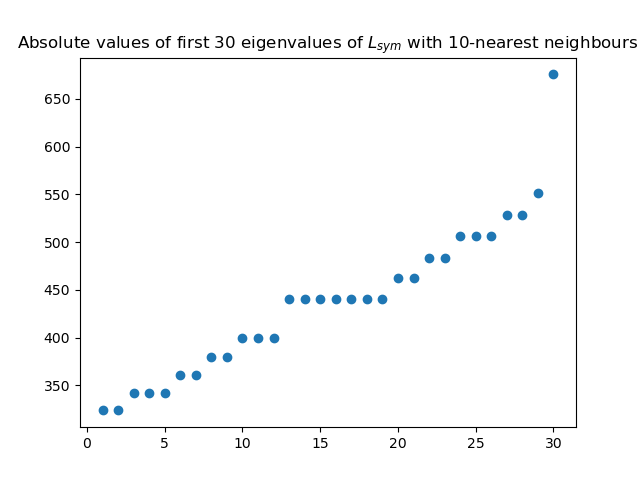
\includegraphics[width=0.5\textheight]{specClustering_l2_k10.png}
			\caption{Ergebnis des spektralen Clusterings unter Verwendung der Euklidischen Distanz und k=10 Nachbarn}
		\end{center}
	\end{figure}
	
	\noindent \textbf{Clustering(euklidisch):}
	$(tn, fp, fn, tp) = 1650, 0, 386, 427)$\\
	\\
	\noindent \textbf{Clustering(GWD):}
	\begin{figure}[h]
		\begin{center}
			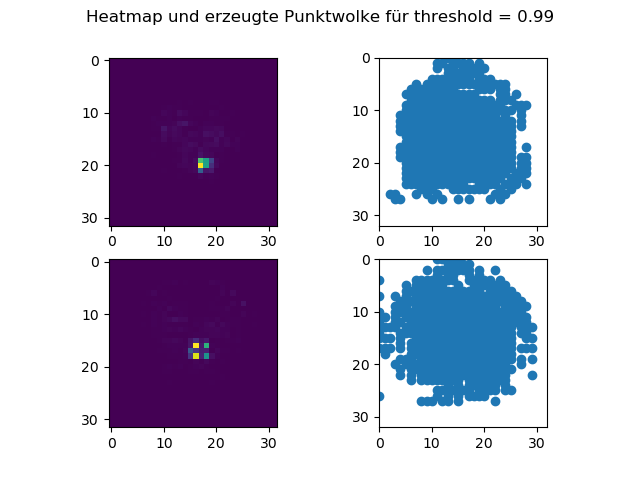
\includegraphics[width=0.5\textheight]{HeatmapPunktwolke99.png}
			\caption{Auswahl der relevantesten Pixel (bis zu $99\%$ der Gesamtmasse) zweier Heatmaps}
		\end{center}
	\end{figure}
	
	\begin{figure}[h]
		\begin{center}
			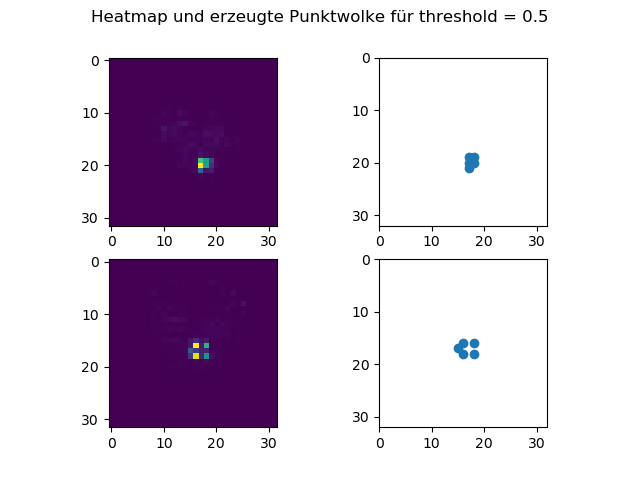
\includegraphics[width=0.5\textheight]{HeatmapPunktwolke50.png}
			\caption{Auswahl der relevantesten Pixel (bis zu $50\%$ der Gesamtmasse) zweier Heatmaps}
		\end{center}
	\end{figure}
	
	\begin{figure}[h]
		\begin{center}
			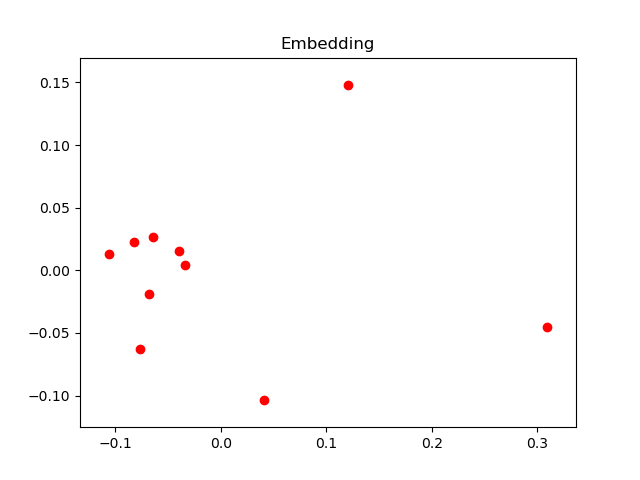
\includegraphics[width=0.5\textheight]{bary_embedding99.png}
			\caption{Einbettung des Baryzentrums mithilfe von Multidimensionaler Skalierung(MDS) bei der Wahl von $99\%$ der Gesamtmasse}
		\end{center}
	\end{figure}
	
	
	
	
	\begin{table}[ht]
		
		
		\begin{center}
			\begin{tabular}{|l|c|c|c|c|}
				\hline
				Seitenlänge des Triggers& Prozentualer Anteil & AER & GUD & num. korrumpierte Daten \\ \hline
				s=2 & 0.000625 & 0.01333333  & 0.962  & 1 \\
				& 0.00125 & 0.356  & 0.964  & 2 \\
				& 0.0025 & 0.576 & 0.97 & 4 \\
				& 0.005 & 0.99867 & 0.962 & 8 \\
				& 0.01 & 0.92 & 0.962 & 17 \\
				& 0.02 & 1.0 & 0.964 & 34\\ 
				& 0.10 & 1.0 & 0.968 & 291\\
				& 0.15 & 1.0 & 0.968 & 436 \\ 
				& 0.33 & 1.0 & 0.968 & 813 \\ \hline
				s=3 & ? & ? & ? &? \\
				& 0.00125 & 34.26 & 96.2 & 2\\
				& 0.0025 & 85.07 & 96.5 & 4\\
				& 0.005	&1.0&96.9& 8 \\ 
				& 0.01 & 1.0 & 0.962& 17 \\
				& 0.05 & 1.0 & 0.966 & 87 \\
				& 0.15 & 1.0 & 0.961& \\ \hline
				s=1 & 0.33 & 1.0 & 0.966 & 813 \\ \hline
			\end{tabular}
			\caption{Qualität der Angriffe auf das Inception v3-Netz mit Stickern Seitenlänge 2 und 3 Pixel bei unterschiedlich großen Anteilen an korrumpierten Daten}
			\label{tab:SPA_incv3}	
		\end{center}
	\end{table}
	
	\begin{remark}
		Für größere Netzwerke ist es einfacher, erfolgreiche Angriffe zu implementieren, auch schon mit weniger korrumpierten Daten.\\
		Vermutung: Die Detektion mittels Clustering funktioniert für eine größere Anzahl an korrumpierten Daten besser. Wenn wir also nur perfekte Angriffe verteidigen wollen, d.h AER=100.00 funktioniert das bei kleineren Netzwerken besser.
	\end{remark}
	\subsubsection{Label-konsistente Poisoning-Angriffe}

	
	\begin{remark}
		Für einen einzelnen Amplitudensticker mit d=10 ist das eigentlich identisch zu dem Angriff mit dem Sticker
	\end{remark}
	0.7        0.86111111 0.85066667 0.81111111 0.66666667        nan
	0.42       0.72888889 0.60888889 0.77083333 0.40757576 0.46666667
	0.69855072 0.88472222 0.53333333 0.74285714 0.39333333 0.67222222
	0.75128205 0.11666667 0.58888889 0.32222222 0.425      0.18
	0.44444444 0.44375    0.8        0.71666667 0.56       0.86666667
	0.11333333 0.3        0.71666667 0.5047619  0.23333333 0.44358974
	0.63333333 0.58333333 0.46666667 0.01111111 0.5        0.36666667
	0.67777778
	$CLP\_amplitudesticker4\_pp33\_eps1200\_d10amp32$
	Jetzt dasselbe noch für nur !!!einen!!! Sticker mit derselben Amplitude am selben Ort
	$'CLP_amplitudesticker_pp33_eps1200_d10amp32'$
	[0.         0.00833333 0.00133333 0.03555556 0.01666667        nan
	0.         0.         0.00222222 0.         0.         0.
	0.05362319 0.00138889 0.0037037  0.         0.         0.025
	0.         0.         0.         0.         0.         0.
	0.         0.         0.         0.05       0.         0.
	0.         0.         0.         0.         0.         0.00512821
	0.         0.         0.         0.         0.         0.
	0.        ]
	
	Dann noch mit amp=16 wieder 4 sticker mit d=10
	$CLP_amplitudesticker4_pp33_eps1200_d10amp16$
	0.11666667 0.23055556 0.26       0.55333333 0.43333333        nan
	0.23333333 0.28444444 0.11555556 0.07708333 0.15       0.0952381
	0.4173913  0.41527778 0.40740741 0.45238095 0.01333333 0.35833333
	0.29487179 0.         0.         0.04444444 0.05       0.01333333
	0.4        0.29791667 0.13888889 0.23333333 0.11333333 0.3
	0.06       0.02962963 0.11666667 0.65714286 0.475      0.71794872
	0.50833333 0.43333333 0.35652174 0.45555556 0.27777778 0.
	0.51111111
	Accuracy on test Dataset: 0.958 
	
	Jetzt: $CLP_amplitudesticker4_pp33_eps1200_d10amp255$
	0.71666667 0.78333333 0.80266667 0.99333333 0.9469697         nan
	0.96       0.97555556 0.98444444 1.         1.         0.25714286
	0.98985507 0.86111111 0.94444444 0.99047619 0.91333333 0.51666667
	0.84871795 0.86666667 0.52222222 0.57777778 0.75       0.67333333
	0.95555556 0.725      0.98888889 0.88333333 0.45333333 0.82222222
	0.81333333 1.         0.98333333 0.4952381  0.26666667 0.92820513
	0.63333333 0.81666667 0.77681159 0.33333333 0.74444444 0.91666667
	0.83333333
	Accuracy on test Dataset: 0.959 
	
	$CLP_amplitudesticker4_pp33_dist10_amp64$ eps300
	[0.8        0.98888889 0.99733333 1.         1.                nan
	1.         1.         0.99555556 0.97916667 0.99545455 0.8047619
	1.         0.99861111 0.92222222 1.         0.99333333 0.98888889
	0.98717949 0.93333333 0.86666667 0.93333333 0.975      0.83333333
	0.96666667 0.93958333 1.         1.         0.98       1.
	0.98       0.97777778 1.         0.92380952 0.55       0.93076923
	0.70833333 0.85       0.82173913 1.         0.8        1.
	1.        
	
	$CLP_amplitudesticker4_pp33_dist10_amp32$
	0.7        0.86111111 0.85066667 0.81111111 0.66666667        nan
	0.42       0.72888889 0.60888889 0.77083333 0.40757576 0.46666667
	0.69855072 0.88472222 0.53333333 0.74285714 0.39333333 0.67222222
	0.75128205 0.11666667 0.58888889 0.32222222 0.425      0.18
	0.44444444 0.44375    0.8        0.71666667 0.56       0.86666667
	0.11333333 0.3        0.71666667 0.5047619  0.23333333 0.44358974
	0.63333333 0.58333333 0.46666667 0.01111111 0.5        0.36666667
	0.67777778
	Accuracy on test Dataset: 0.959 
	
	
	$CLP_amplitudesticker4_pp33_dist10_amp16$
	0.11666667 0.23055556 0.26       0.55333333 0.43333333        nan
	0.23333333 0.28444444 0.11555556 0.07708333 0.15       0.0952381
	0.4173913  0.41527778 0.40740741 0.45238095 0.01333333 0.35833333
	0.29487179 0.         0.         0.04444444 0.05       0.01333333
	0.4        0.29791667 0.13888889 0.23333333 0.11333333 0.3
	0.06       0.02962963 0.11666667 0.65714286 0.475      0.71794872
	0.50833333 0.43333333 0.35652174 0.45555556 0.27777778 0.
	0.51111111]
	Performance of poisoned net on unpoisoned training data:
	loss on test dataset: 0.19637071904851583
	Accuracy on test Dataset: 0.958 
	
	\begin{figure}[h]
		\begin{center}
			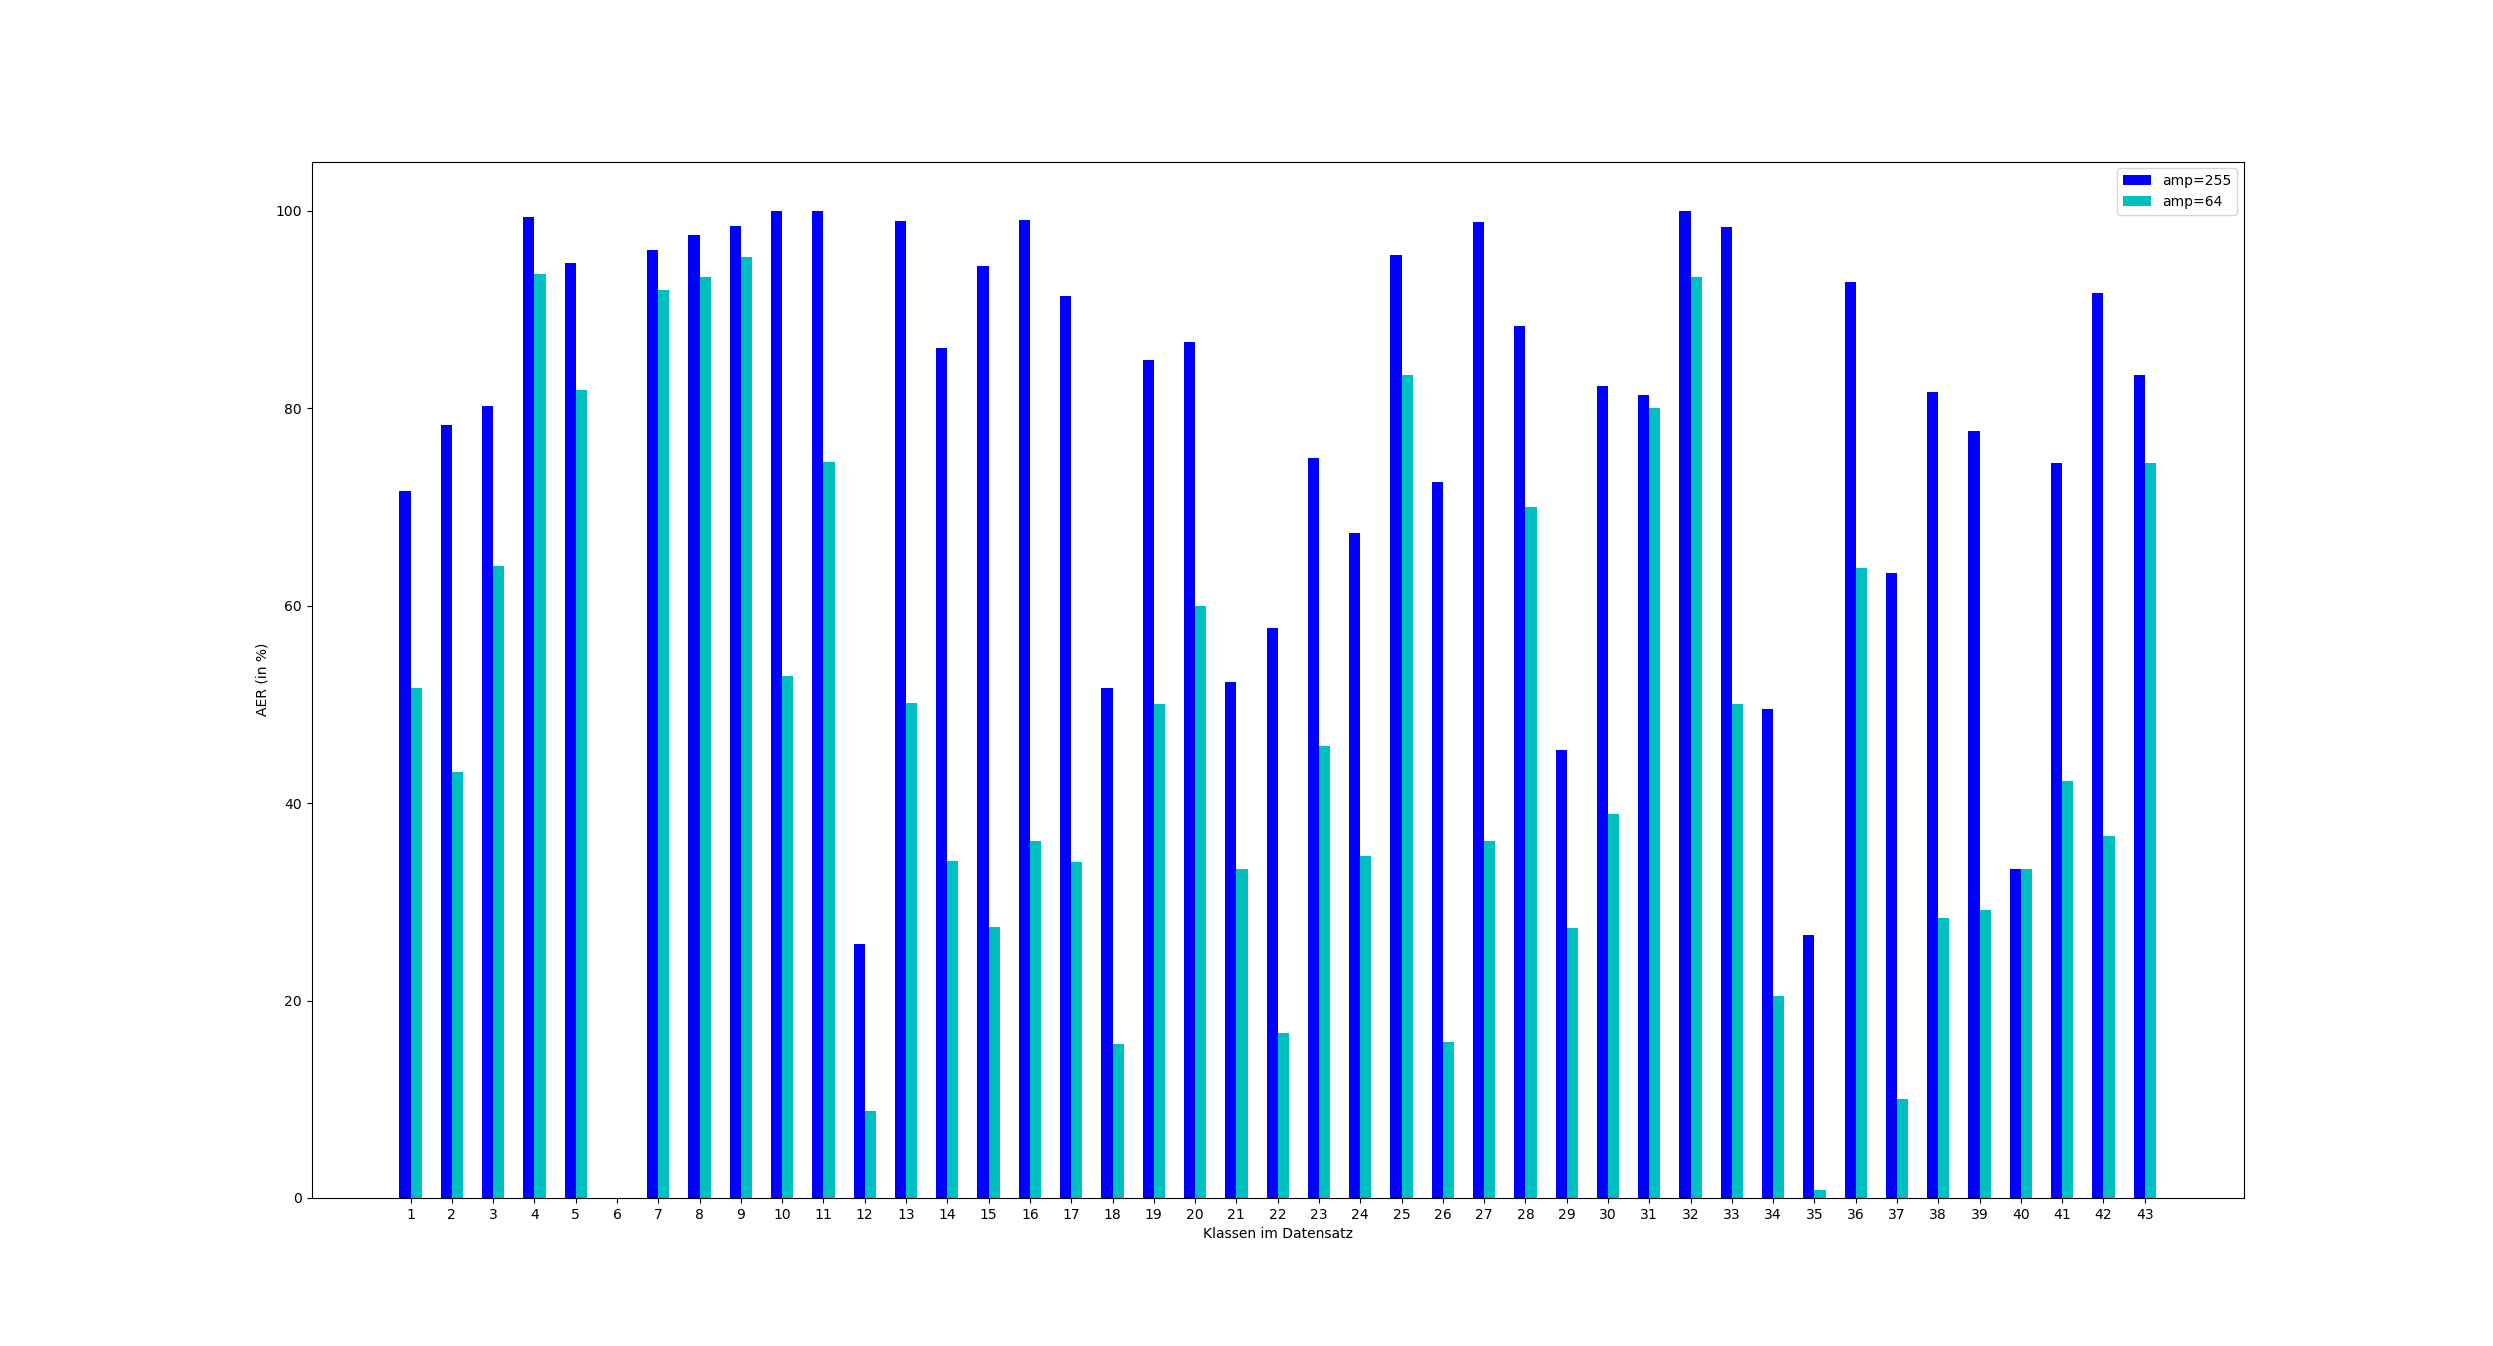
\includegraphics[width=0.5\textheight]{Vergleich_AER_CLPA.png}
			\caption{Angriffserfolgsrate pro Klasse bei Clean-Label-Poisoning-Attacks für verschiedene Werte \textit{amp} des Amplitudenstickers in vierfacher Ausführung bei Abstand $d=10$ zum Rand}
			\label{fig:AER_proKlasse_CLPA}
		\end{center}
	\end{figure}
	
	In \autoref{fig:AER_proKlasse_CLPA} sind die Angriffserfolgsraten pro Klasse im Fall von $33 \%$ korrumpierten Daten und dem Amplitudensticker in jeder der 4 Bildecken mit dem Abstand von 10 Pixeln zum Rand dargestellt. In beiden Fällen geben wir keine AER für die Klasse 6 an, über die der Angriff stattfindet.
	Die mittlere Angriffserfolgsrate beträgt für $amp=255$ $79.15 \%$. In mehreren Klassen wird eine AER von $100 \%$ erreicht.\\
	Für $amp=64$ fällt der Angriff mit einer mAER von $48.17 \%$ deutlich schwächer aus. Die maximal erreichte AER beträgt $95.33 \%$ in Klasse 10. Die minimalen AER sind $25 \%$ bzw. $0.83 \% $.
	Eine weitere Reduktion der Amplitude auf $amp=32$ führt zu einer mAER von $6.55 \%$ und einer maximalen AER von $33 \%$.
	
	Für d=0, amplitude=64 und eps=1200 ergibt sich kein erfolgreicher Angriff, dabei war fast alles 0, die Trigger im Testdatensatz waren auch auf 64
	Jetzt für d=10, auch hier gilt amp=64 im Testdatensatz:Ergebnis:
	
	
	------------------------------------
	\subsection{Activation Clustering}
	\subsection{Räumliche Transformationen}
	\begin{itemize}
		\item ASR ist sehr stark vom Ort des Triggers abhängig.
		\item Ort des Triggers kann nicht direkt geändert werden.
		\item Benutze Transformationen(Flipping, Scaling), um den Trigger wirkungslos zu machen.
		\item Somit kann die ASR während der Inferenz verringert werden. Es lässt sich aber keine Auussage darüber treffen, ob ein Angriff vorliegt
	\end{itemize}
	\newpage
	\section{Weitere mögliche Schritte} \label{chapter_weitereSchritte}
	\begin{itemize}
		\item Untersuchung der Detektionsqualität in Abhängigkeit von $\varepsilon$
		\item Automatische Platzierung des Auslösers an fest gewählter Position auf dem Verkehrsschild anstatt zufälligem Platzieren in einem Fenster mit vorher festgelegter Größe. In \cite{badnets} wird  Faster-RCNN (F-RCNN) zur Klassifikation des LISA-Datensatzes\footnote{\url{http://cvrr.ucsd.edu/LISA/lisa-traffic-sign-dataset.html}} benutzt. Es ist die Aufgabe, die Verkehrsschilder in die 3 Superklassen Stoppschild, Geschwindigkeitsbegrenzung und Warnschild einzuteilen. Der Datensatz enthält zudem die BoundingBoxen, sodass der Auslöser genauer angebracht werden kann.
		\item Verbesserte Version der Layer-wise Relevance Propagation
		\item Untersuchung anderer Verfahren, die die Interpretierbarkeit ermöglichen, beispielsweise: VisualBackProp: efficient visualization of CNNs\footnote{\url{https://arxiv.org/abs/1611.05418}}
		\item Vergleich mit Cifar-10/Cifar-100 Datensatz\footnote{\url{https://www.cs.toronto.edu/~kriz/cifar.html}}\footnote{\url{https://www.cs.toronto.edu/~kriz/learning-features-2009-TR.pdf}}
	\end{itemize}
	
	
	\section{Zusammenfassung und Ausblick} \label{chapter_conclusion}
	Beobachtung: Je größer die Netzwerke sind, desto leichter lassen sich Poisoning-Angriffe realisieren.
	
	\printglossaries
	\newpage
	\appendix
	\section{Verwendete Netzwerke}
	\subsection{Net}
	
	\begin{lstlisting}[language=Python, caption=Kleines Netzwerk]
	
	class Net(nn.Module):
	
	def __init__(self, ):
	super(Net, self).__init__()
	self.size = 64 * 4 * 4
	self.conv1 = nn.Conv2d(in_channels=3, out_channels=12, kernel_size=5, padding=2)
	self.pool = nn.MaxPool2d(kernel_size=2, stride=2)
	self.conv1_in = nn.InstanceNorm2d(12)
	self.conv2 = nn.Conv2d(in_channels=12, out_channels=32, kernel_size=5, padding=2)
	
	self.conv2_bn = nn.BatchNorm2d(32)
	
	self.conv3 = nn.Conv2d(in_channels=32, out_channels=64, kernel_size=5, padding=2)
	
	self.fc1 = nn.Linear(self.size, 256)
	self.fc1_bn = nn.BatchNorm1d(256)
	self.fc2 = nn.Linear(256, 128)
	self.fc3 = nn.Linear(128, 43)
	
	
	def forward(self, x):
	x = self.pool(F.relu(self.conv1_in(self.conv1(x))))
	x = self.pool(F.relu(self.conv2_bn(self.conv2(x))))
	x = self.pool(F.relu(self.conv3(x)))
	x = x.view(-1, self.size)
	x = F.relu(self.fc1_bn(self.fc1(x)))
	x = F.dropout(x)
	xx = F.relu(self.fc2(x))
	x = F.dropout(xx)
	x = self.fc3(x)
	
	return x, xx
	
	\end{lstlisting}
	
	\begin{lstlisting}[language=Python, caption=Einfachere Version von Inception v3]
	InceptionNet3(
	(features): Sequential(
	(0): InceptionA(
	(parallel_dummyA): New_parallel_chain_dummy()
	(conv1x1): BatchConv(
	(conv): Conv2d(3, 64, kernel_size=(1, 1), stride=(1, 1))
	(bn): BatchNorm2d(64, eps=1e-05, momentum=0.1, affine=True, track_running_stats=True)
	(relu): ReLU()
	)
	(parallel_dummyB): New_parallel_chain_dummy()
	(conv5x5_1): BatchConv(
	(conv): Conv2d(3, 48, kernel_size=(1, 1), stride=(1, 1))
	(bn): BatchNorm2d(48, eps=1e-05, momentum=0.1, affine=True, track_running_stats=True)
	(relu): ReLU()
	)
	(conv5x5_2): BatchConv(
	(conv): Conv2d(48, 64, kernel_size=(5, 5), stride=(1, 1), padding=(2, 2))
	(bn): BatchNorm2d(64, eps=1e-05, momentum=0.1, affine=True, track_running_stats=True)
	(relu): ReLU()
	)
	(parallel_dummyC): New_parallel_chain_dummy()
	(conv3x3dbl_1): BatchConv(
	(conv): Conv2d(3, 64, kernel_size=(1, 1), stride=(1, 1))
	(bn): BatchNorm2d(64, eps=1e-05, momentum=0.1, affine=True, track_running_stats=True)
	(relu): ReLU()
	)
	(conv3x3dbl_2): BatchConv(
	(conv): Conv2d(64, 96, kernel_size=(3, 3), stride=(1, 1), padding=(1, 1))
	(bn): BatchNorm2d(96, eps=1e-05, momentum=0.1, affine=True, track_running_stats=True)
	(relu): ReLU()
	)
	(conv3x3dbl_3): BatchConv(
	(conv): Conv2d(96, 96, kernel_size=(3, 3), stride=(1, 1), padding=(1, 1))
	(bn): BatchNorm2d(96, eps=1e-05, momentum=0.1, affine=True, track_running_stats=True)
	(relu): ReLU()
	)
	(parallel_dummyD): New_parallel_chain_dummy()
	(pool): MaxPool2d(kernel_size=3, stride=1, padding=1, dilation=1, ceil_mode=False)
	(pool1x1): BatchConv(
	(conv): Conv2d(3, 32, kernel_size=(1, 1), stride=(1, 1))
	(bn): BatchNorm2d(32, eps=1e-05, momentum=0.1, affine=True, track_running_stats=True)
	(relu): ReLU()
	)
	(parallel_dummyE): New_parallel_chain_dummy()
	(cat): Cat()
	)
	(1): MaxPool2d(kernel_size=2, stride=2, padding=0, dilation=1, ceil_mode=False)
	(2): BatchConv(
	(conv): Conv2d(256, 256, kernel_size=(2, 2), stride=(1, 1))
	(bn): BatchNorm2d(256, eps=1e-05, momentum=0.1, affine=True, track_running_stats=True)
	(relu): ReLU()
	)
	(3): MaxPool2d(kernel_size=2, stride=2, padding=0, dilation=1, ceil_mode=False)
	(4): BatchConv(
	(conv): Conv2d(256, 256, kernel_size=(2, 2), stride=(1, 1))
	(bn): BatchNorm2d(256, eps=1e-05, momentum=0.1, affine=True, track_running_stats=True)
	(relu): ReLU()
	)
	(5): MaxPool2d(kernel_size=2, stride=2, padding=0, dilation=1, ceil_mode=False)
	(6): BatchConv(
	(conv): Conv2d(256, 256, kernel_size=(2, 2), stride=(1, 1))
	(bn): BatchNorm2d(256, eps=1e-05, momentum=0.1, affine=True, track_running_stats=True)
	(relu): ReLU()
	)
	(7): MaxPool2d(kernel_size=2, stride=2, padding=0, dilation=1, ceil_mode=False)
	)
	(classifiers): Sequential(
	(0): Linear(in_features=256, out_features=256, bias=True)
	(1): ReLU(inplace=True)
	(2): Dropout(p=0.5, inplace=False)
	(3): Linear(in_features=256, out_features=128, bias=True)
	(4): ReLU(inplace=True)
	(5): Dropout(p=0.5, inplace=False)
	(6): Linear(in_features=128, out_features=43, bias=True)
	)
	)
	\end{lstlisting}
	Aufbau dieses Netzwerkes:
	1. Inception-Modul
	2. [pool1, batchConv1, pool2, batchConv2, pool3, batchConv3, pool4]
	3. Drei Lineare Schichten mit ReLu und Dropout dazwischen
	
	Im Unterschied zum offiziellen Inception Netz(v1v2v3) gibt es in dieser 
	vereinfachten Version keinen "stem" aus convs, 
	es geht direkt mit InceptionA los.
	
	Wie ähnlich sind sich InceptionA(hier) und das offizielle InceptionA-Modul?
	\begin{lstlisting}[language=Python, caption=Reversed Model incv3]
	
	[Linear(in_features=128, out_features=43, bias=True), 
	Dropout(p=0.5, inplace=False), 
	ReLU(inplace=True), 
	Linear(in_features=256, out_features=128, bias=True), 
	Dropout(p=0.5, inplace=False), 
	ReLU(inplace=True), 
	Linear(in_features=256, out_features=256, bias=True), 
	MaxPool2d(kernel_size=2, stride=2, padding=0, dilation=1, ceil_mode=False), 
	ReLU(), 
	BatchNorm2d(256, eps=1e-05, momentum=0.1, affine=True, track_running_stats=True), Conv2d(256, 256, kernel_size=(2, 2), stride=(1, 1)), 
	MaxPool2d(kernel_size=2, stride=2, padding=0, dilation=1, ceil_mode=False), 
	ReLU(), 
	BatchNorm2d(256, eps=1e-05, momentum=0.1, affine=True, track_running_stats=True), Conv2d(256, 256, kernel_size=(2, 2), stride=(1, 1)), 
	MaxPool2d(kernel_size=2, stride=2, padding=0, dilation=1, ceil_mode=False), 
	ReLU(), BatchNorm2d(256, eps=1e-05, momentum=0.1, affine=True, track_running_stats=True), 
	Conv2d(256, 256, kernel_size=(2, 2), stride=(1, 1)), 
	MaxPool2d(kernel_size=2, stride=2, padding=0, dilation=1, ceil_mode=False),
	
	[[Conv2d(3, 64, kernel_size=(1, 1), stride=(1, 1)), 
	BatchNorm2d(64, eps=1e-05, momentum=0.1, affine=True, track_running_stats=True), ReLU()], 
	
	[Conv2d(3, 48, kernel_size=(1, 1), stride=(1, 1)), 
	BatchNorm2d(48, eps=1e-05, momentum=0.1, affine=True, track_running_stats=True), ReLU(), Conv2d(48, 64, kernel_size=(5, 5), stride=(1, 1), padding=(2, 2)), BatchNorm2d(64, eps=1e-05, momentum=0.1, affine=True, track_running_stats=True), ReLU()], 
	
	[Conv2d(3, 64, kernel_size=(1, 1), stride=(1, 1)), 
	BatchNorm2d(64, eps=1e-05, momentum=0.1, affine=True, track_running_stats=True), ReLU(), 
	Conv2d(64, 96, kernel_size=(3, 3), stride=(1, 1), padding=(1, 1)), 
	BatchNorm2d(96, eps=1e-05, momentum=0.1, affine=True, track_running_stats=True), ReLU(), 
	Conv2d(96, 96, kernel_size=(3, 3), stride=(1, 1), padding=(1, 1)), 
	BatchNorm2d(96, eps=1e-05, momentum=0.1, affine=True, track_running_stats=True), ReLU()], 
	
	[MaxPool2d(kernel_size=3, stride=1, padding=1, dilation=1, ceil_mode=False), Conv2d(3, 32, kernel_size=(1, 1), stride=(1, 1)), 
	BatchNorm2d(32, eps=1e-05, momentum=0.1, affine=True, track_running_stats=True), 
	ReLU()], 
	
	[Cat()]]]
	\end{lstlisting}
	\section{Parameter für Training und Einlesen der Daten}\label{param_net}
	Die in \cite{CH} gewählten Parameter wären ein guter Ausgangspunkt.\\
	Für das Einlesen der Daten benutzen wir, sofern nicht weiter angegeben die folgenden Augmentierungen:
	
	\begin{lstlisting}[language=Python, caption=Augemntierung beim Einlesen der Daten]
	__train_transform = transforms.Compose(
	[
	transforms.RandomResizedCrop((image_size, image_size), 
	scale=(0.6, 1.0)),
	transforms.RandomRotation(degrees=15),
	transforms.ColorJitter(brightness=0.1, contrast=0.1, 
	saturation=0.1, hue=0.1),
	transforms.RandomAffine(15),
	transforms.RandomGrayscale(),
	transforms.Normalize(	mean=[0.485, 0.456, 0.406], 
	std=[0.229, 0.224, 0.225]),
	transforms.ToTensor()
	
	]
	
	
	
	\end{lstlisting}
	Die Werte von mean und std variieren für alle ausgeführten Poisoning-Angriffe. Anstatt beide jedes Mal erneut zu berechnen, verwenden wir die von pytorch angegebenen Werte \footnote{\url{https://github.com/pytorch/examples/blob/97304e232807082c2e7b54c597615dc0ad8f6173/imagenet/main.py\#L197-L198}}, die für die vor-trainierten Modelle empfohlen werden und auf dem Datensatz ImageNet\footnote{\url{https://image-net.org/}} basieren.\\ 
	Wir trainieren die Netzwerke über maximal 100 Epochen und benutzen \textit{early stopping} mit einer $patience=20$. Die verwendete Implementierung ist eine modifizierte Version von Bjarte Mehus Sunde \footnote{\url{https://github.com/Bjarten/early-stopping-pytorch}}, die wiederum auf PyTorch Ignite\footnote{\url{https://github.com/pytorch/ignite/blob/master/ignite/handlers/early\_stopping.pyt}} basiert.\\
	
	\section{Einlesen der Daten bei AC}
	Ohne Transformationen, wie den Testdatensatz.
	
	
	\section{Parameter für die ausgeführten Angriffe}\label{param_attacks}
	Für das projizierte Gradientenverfahren benutzen wir 10 Iterationen und eine Schrittweite von 0.015.
	
	\textbf{Label-konsistente Poisoning-Angriffe:}
	\section{Datensätze}
	GTSRB\footnote{\url{https://benchmark.ini.rub.de/gtsrb_dataset.html}}
	Datensatz Splitting (Train; Val, test)
	
	ImageNet besteht über 14 Millionen Bildern in 100 Klassen.
	\section{Programmcode}
	Der vollständige Programmcode ist verfügbar unter \url{https://github.com/lukasschulth/MA-Detection-of-Poisoning-Attacks}
	
	%\verbatiminput{Netlayout.txt}
	
	%\verbatiminput{InceptionNet3layout.txt}
	\section{Notizen}
	registered spaces \footnote{\url{https://arxiv.org/pdf/1809.06422.pdf}}
	Barycenters in the Wasserstein Space\footnote{\url{https://arxiv.org/pdf/1809.06422.pdf}}\\
	Was passiert bei der Kombination von 2 verschiedenen Triggern? Einmal keine Überlappung(d.h. 2verschiedene Trigger auf dem selben Bild) vs. auch beide Trigger auf einem Bild ist zulässig.
	\newpage
	
	\printglossaries
	
	\newpage
	
	\bibliographystyle{alpha}
	
	\bibliography{bibfileMAlukasschulth}
	
	
	
\end{document}